%%%%%%%%%%%%%%%%%%%%%%%%%%%%%%%%%%%%%%%%%
% Masters/Doctoral Thesis
% LaTeX Template
% Version 2.5 (27/8/17)
%
% This template was downloaded from:
% http://www.LaTeXTemplates.com
%
% Version 2.x major modifications by:
% Vel (vel@latextemplates.com)
%
% This template is based on a template by:
% Steve Gunn (http://users.ecs.soton.ac.uk/srg/softwaretools/document/templates/)
% Sunil Patel (http://www.sunilpatel.co.uk/thesis-template/)
%
% Template license:
% CC BY-NC-SA 3.0 (http://creativecommons.org/licenses/by-nc-sa/3.0/)
%
%%%%%%%%%%%%%%%%%%%%%%%%%%%%%%%%%%%%%%%%%

%------------------------------------
%	PACKAGES AND OTHER DOCUMENT CONFIGURATIONS
%------------------------------------

\documentclass[
11pt, % The default document font size, options: 10pt, 11pt, 12pt
oneside, % Two side (alternating margins) for binding by default, uncomment to switch to one side
british, % ngerman for German
onehalfspacing, % Single line spacing, alternatives: onehalfspacing or doublespacing
%draft, % Uncomment to enable draft mode (no pictures, no links, overfull hboxes indicated)
%nolistspacing, % If the document is onehalfspacing or doublespacing, uncomment this to set spacing in lists to single
liststotoc, % Uncomment to add the list of figures/tables/etc to the table of contents
%toctotoc, % Uncomment to add the main table of contents to the table of contents
parskip, % Uncomment to add space between paragraphs
%nohyperref, % Uncomment to not load the hyperref package
headsepline, % Uncomment to get a line under the header
%chapterinoneline, % Uncomment to place the chapter title next to the number on one line
%consistentlayout, % Uncomment to change the layout of the declaration, abstract and acknowledgements pages to match the default layout
usenames,
dvipsnames % load default colors
]{MastersDoctoralThesis} % The class file specifying the document structure

%\includeonly{parts/titlepage}
%\includeonly{chapters/2_obs}
%\includeonly{chapters/3_itaobs}
%\includeonly{chapters/4_methods}
%\includeonly{chapters/5_validation}
%\includeonly{chapters/6_conclusions}
%\includeonly{appendices/appendixA}
%\includeonly{appendices/appendixB}

\usepackage[utf8]{inputenc} % Required for inputting international characters
\usepackage[T1]{fontenc} % Output font encoding for international characters

\usepackage{mathpazo} % Use the Palatino font by default

\usepackage{amsmath} % better math

\usepackage{soul} % \hl for highlighting

\usepackage[
    backend=bibtex, %biber fails
    style=authoryear-comp,
    natbib=true,
    maxbibnames=9,
    maxcitenames=2,
    %uniquelist=false %https://tex.stackexchange.com/questions/69028/set-limit-to-one-author-when-using-et-al-in-biblatex
]{biblatex} % Use the bibtex backend with the authoryear citation style (which resembles APA)

\addbibresource{mendeley_v2.bib} % The filename of the bibliography

\usepackage[autostyle=true]{csquotes} % Required to generate language-dependent quotes in the bibliography

\usepackage{microtype} %improves the spacing between words and letters

\usepackage{enumitem} % Lets you use letters in enumerate

\usepackage{wrapfig} % wrap text around figures

%\usepackage[nottoc]{tocbibind}%Show Bib in TOC

%\usepackage[dvipsnames]{xcolor} %additional colors

\usepackage{eurosym} %Euro symbol

\usepackage{booktabs} % better tables
\usepackage{rotating} % landscape stuff, such as tables
\usepackage{array} % for m columns
\usepackage{multirow} % multi row tables
\usepackage{bigdelim} % for big braces in tables (https://tex.stackexchange.com/a/129797/66561)

\usepackage[skip=-2pt, position=top, labelfont=normalfont]{subcaption} % multiple figures in one
%skip=-2pt reduces space between caption and subfigure
%singlelinecheck=false, justification=raggedright move the caption to the left

\usepackage{microtype}%micro-typographic extension for better looks (subliminal refinements towards typographical perfection)
\usepackage{textcomp}% Solves some warnings....
\usepackage[titletoc, title, header]{appendix}% For nicer appendices

\usepackage{tabularx} % better tables

\usepackage{multicol} % itemizations on multiple columns

\AtEndPreamble{\usepackage[noabbrev]{cleveref}} % Even nicer references and links. Provides \cref. This package should be loaded LAST.

\setcounter{tocdepth}{3} % subsubsections get numbers too!
\setcounter{secnumdepth}{3}

\DeclareSIUnit\month{month}
\DeclareSIUnit{\nothing}{\relax}

%------------------------------------
%	MARGIN SETTINGS
%------------------------------------

\geometry{
	paper=a4paper, % Change to letterpaper for US letter
	inner=2.5cm, % Inner margin
	outer=3.8cm, % Outer margin
	bindingoffset=.5cm, % Binding offset
	top=1.5cm, % Top margin
	bottom=1.5cm, % Bottom margin
	%showframe, % Uncomment to show how the type block is set on the page
}

%------------------------------------
%	THESIS INFORMATION
%------------------------------------

\thesistitle{Climate change impact on flood hazard over Italy} % Your thesis title, this is used in the title and abstract, print it elsewhere with \ttitle
\supervisor{Erika Coppola} % Your supervisor's name, this is used in the title page, print it elsewhere with \supname
\examiner{} % Your examiner's name, this is not currently used anywhere in the template, print it elsewhere with \examname
\degree{Doctor of Philosophy} % Your degree name, this is used in the title page and abstract, print it elsewhere with \degreename
\author{Adriano \textsc{Fantini}} % Your name, this is used in the title page and abstract, print it elsewhere with \authorname
\addresses{} % Your address, this is not currently used anywhere in the template, print it elsewhere with \addressname

\subject{} % Your subject area, this is not currently used anywhere in the template, print it elsewhere with \subjectname
\keywords{flood,climate,chym,netcdf} % Keywords for your thesis, this is not currently used anywhere in the template, print it elsewhere with \keywordnames
\university{\href{https://www.units.it}{University of Trieste}} % Your university's name and URL, this is used in the title page and abstract, print it elsewhere with \univname
\department{\href{https://dmg.units.it/}{Department of Mathematics and Geosciences}} % Your department's name and URL, this is used in the title page and abstract, print it elsewhere with \deptname
\group{\href{https://web.units.it/dottorato/esfm/}{PhD Course in Earth Science, Fluid-Dynamics, and Mathematics, XXXI cycle}} % Your research group's name and URL, this is used in the title page, print it elsewhere with \groupname
\faculty{\href{https://web.units.it/dottorato/esfm/}{PhD Course in Earth Science, Fluid-Dynamics, and Mathematics, XXXI cycle}} % Your faculty's name and URL, this is used in the title page and abstract, print it elsewhere with \facname

\AtBeginDocument{
\hypersetup{pdftitle=\ttitle} % Set the PDF's title to your title
\hypersetup{pdfauthor=\authorname} % Set the PDF's author to your name
\hypersetup{pdfkeywords=\keywordnames} % Set the PDF's keywords to your keywords
\hypersetup{linktocpage} % Links will be numbers, not titles, in TOC
\hypersetup{ %set up some nice colors for links
    citecolor=PineGreen,
    linkcolor=MidnightBlue
}
%\hypersetup{hidelinks} %or hide them, make=ing all them black

\sisetup{detect-all,binary-units,range-units=single}
}

\begin{document}

\frontmatter % Use roman page numbering style (i, ii, iii, iv...) for the pre-content pages

\pagestyle{plain} % Default to the plain heading style until the thesis style is called for the body content

%------------------------------------
%	TITLE PAGE
%------------------------------------

\begin{titlepage}
\begin{center}

\vspace*{.04\textheight}
{\scshape\LARGE \univname\par}\vspace{.5cm} % University name
\includegraphics[width=0.2\textwidth]{figures/logos/logosfondoBIG}\hspace{2cm}
\includegraphics[width=0.2\textwidth]{figures/logos/ICTPLogo}\\
\vspace{.5cm}
\textsc{\Large Doctoral Thesis}\\[0.5cm] % Thesis type

\HRule \\[0.4cm] % Horizontal line
{\huge \bfseries \ttitle\par}\vspace{0.3cm} % Thesis title
\HRule \\[.6cm] % Horizontal line

%\begin{figure}[h!]
%    \centering
    \includegraphics[width=0.4\textwidth]{figures/voronoi}
%\end{figure}

\begin{minipage}[t]{0.4\textwidth}
\begin{flushleft} \large
\emph{Author:}\\
{\authorname} % Author name - remove the \href bracket to remove the link
\end{flushleft}
\end{minipage}
\begin{minipage}[t]{0.4\textwidth}
\begin{flushright} \large
\emph{Supervisor:} \\
\supname
% \href{https://www.ictp.it/phonebook/person?id=2541}{\supname} % Supervisor name - remove the \href bracket to remove the link  
\end{flushright}
\end{minipage}\\[1cm]
 
\vfill

% \large \textit{A thesis submitted in fulfillment of the requirements\\ for the degree of \degreename}\\[0.3cm] % University requirement text
% \textit{in the}\\[0.4cm]
% \\[0.4cm]
\groupname\\\deptname\\[2cm] % Research group name and department name
 
%\vfill

%{\large \today}\\[4cm] % Date
%\includegraphics{Logo} % University/department logo - uncomment to place it
 
\vfill
\end{center}
\end{titlepage}

%------------------------------------
%	DECLARATION PAGE
%------------------------------------

% \include{parts/declaration}

%------------------------------------
%	QUOTATION PAGE
%------------------------------------

\vspace*{0.2\textheight}

\noindent\enquote{\itshape There is a pleasure in the pathless woods\\
   There is a rapture on the lonely shore\\
   There is society where none intrudes\\
   By the deep Sea, and music in its roar:\\
   I love not Man the less, but Nature more}\bigbreak

\hfill George Byron

%------------------------------------
%	ABSTRACT PAGE
%------------------------------------

\begin{abstract}
\addchaptertocentry{\abstractname} % Add the abstract to the table of contents
Floods are one of the most devastating natural disasters, with strong impacts on both society and economy.
Flood hazard estimation is an essential tool for protecting the population from floods both financially, via insurance policies, and physically, via water management and engineering.
In Europe, different kinds of flood maps are usually produced with different methods by governments, regional agencies, or insurance and re-insurance companies.
In the last decades, however, new approaches based on hydrological and hydraulical modelling emerged as viable, which allows for a more robust and reproducible physically-based estimation of flood extent and water level.
In this work a multimodel approach has been adopted, with a hydrological model  driven by multiple sources of precipitation input data, generating discharge data for a given region or basin for a long time period.
The discharge is then fed to a hydrodynamic model which produces of flood extents and, if necessary, other variables such as flood depth or flow speed.
Extreme value analysis is also used to derive any Return Period value (ranging from 10 to 500 years) starting from a shorter observational record, by assuming a given distribution for extreme events.

Over Italy, flood hazard has not yet been evaluated using a unified method.
We propose a methodology to simulate flood hazard for any return period, based on a model chain comprised of three models: the Regional Climate Model RegCM, the hydrological model CHyM and the hydraulical model CA2D.
For the time being only domains covering the complete Italian territory were simulated, but no limitation is in place that would prevent this technique from being applied to any domain worldwide, provided that the necessary input data is available.

In order to provide observed precipitation data as input to the hydrological model, we created a new product called GRIPHO (GRidded Italian Precipitation Hourly Observations), which consists of quality checked hourly precipitation observations over the complete Italian territory.
We validate GRIPHO against other state-of-the-art precipitation datasets over Italy, showing good performance in reproducing both mean and extreme precipitation: GRIPHO is comparable with the high resolution ARCIS and EURO4M-APGD datasets in Northern Italy, and shows finer spatial details and more consistent extremes than E-OBS in the rest of the domain.

Two regional climate simulations, one run in perfect boundary mode (with ERA-Interim) and one a scenario simulation (driven with  HadGEM, RCP8.5), are described and validated over the Italian territory.
Both simulations show good agreement with observation in several precipitation and temperature metrics, for both extreme and mean climate.
The projected climate change signal is also evaluated, finding, on average, increased extreme precipitation even in areas where mean precipitation decreases.

Three hydrological simulations, driven by both observations and regional climate  model outputs, are described.
Validation is carried out against a set of discharge stations, finding generally good performance of the CHyM model for the regions where observations are available.
Using different metrics, we assess the future changes in mean and extreme discharge for the Italian territory, finding strong increases in possible flood proxies.
In particular, mean discharge is projected to increase (decrease) in Northern Italy in winter (summer), which is directly linked to changes in mean precipitation over the Po river basin.
In winter and autumn, maximum yearly discharges increase by 50\% in several Italian regions, with summer and spring showing more mixed results.
100-year Return Period discharges are projected to increase over most of Italy by more than 100\% by the end of the century.
Similarly, the frequency of exceedance of extreme discharge thresholds drastically increases in the future scenario compared to the reference period, with changes for the 100-year threshold exceeding 500\% for several rivers in Italy, including the Po river.

Finally, we present preliminary results over the whole Italian territory for flood maps for different Return Periods, as produced by a hydraulic model fed by simulated discharge data.
The resulting maps are compatible with the currently available products obtained from regional environment agencies, but have the advantage of being produced with a coherent, scientific methodology.
\end{abstract}

%------------------------------------
%	ACKNOWLEDGEMENTS
%------------------------------------

\begin{acknowledgements}
\addchaptertocentry{\acknowledgementname} % Add the acknowledgements to the table of contents
This PhD project is the outcome of the work of many people: the core team was composed by Erika Coppola, Francesca Raffaele, Rita Nogherotto and myself. Graziano Giuliani and Fabio di Sante also were instrumental to several parts of the project thanks to their technical insight. 

Whenever fitting, specific acknowledgements are given inside the text or in footnotes, but here I would especially like to thank all of my colleagues at the ICTP Earth System Physics group, which funded the project and hosted me during my PhD.\\
In particular, I thank Rita, Francesca and Erika, for sharing this adventure with me: thanks for being patient when I was stubborn, for being understanding when I made mistakes.
I can only imagine it's not always easy to work with a pedantic and introvert person like myself.\\
Thanks to Graziano and Ivan, without whom the mysteries of computing would often have remained just that: mysteries.
I thank the colleagues and friends of a time now gone, Bianca, Csaba, Stefano, Ramon, Irene: our paths have crossed, and I hope they will again.

But most of all I want to thank those who, during these three years, more than colleagues have been friends.
Giorgio, for putting up with me all this time; Fabio, for teaching by example (to play table football, of course); Costanza, for that one ice cream, and for more to come; James, for being the most down to cheese guy; Rita once again, for the moral support and the reality checks in harsh times; Marco, for the smile always ready.\\
Thank you, friends, for the most important thing: because you made going to work not a chore, but a pleasure. 
% Well... most of the time, anyway!

I have a short memory. I am certain I am forgetting someone, and if that's you, reader, I beg your pardon. If you think you deserve my gratitude, well, you probably do: thank you.

\newpage
\section*{Author's note}
This thesis has been compressed for uploading and is missing hyperlinks.
The original version, containing full-resolution images and hyperlinks, can be obtained from \url{http://users.ictp.it/~afantini/PhD_thesis/PhD_thesis.pdf} or by requesting it to \href{mailto:adr.fantini@gmail.com}{adr.fantini@gmail.com}.


\end{acknowledgements}

%------------------------------------
%	LIST OF CONTENTS/FIGURES/TABLES PAGES
%------------------------------------

\tableofcontents % Prints the main table of contents

\listoffigures % Prints the list of figures

\listoftables % Prints the list of tables

%------------------------------------
%	ABBREVIATIONS
%------------------------------------

%\begin{abbreviations}{ll} % Include a list of abbreviations (a table of two columns)

\textbf{RP}  & \textbf{R}eturn \textbf{P}eriod\\
\textbf{FFA} & \textbf{F}lood \textbf{F}requency \textbf{A}nalysis\\
\textbf{FDC} & \textbf{F}low \textbf{D}uration \textbf{C}urve\\
\textbf{FDF} & \textbf{F}low \textbf{D}uration \textbf{F}requency\\
\textbf{SDH} & \textbf{S}ynthetic \textbf{D}esign \textbf{H}ydrograph\\
\textbf{RCM} & \textbf{R}egional \textbf{C}limate \textbf{M}odel\\
\textbf{GCM} & \textbf{G}lobal \textbf{C}limate \textbf{M}odel\\
\textbf{RESM} & \\
\textbf{CMIP} & \\
\textbf{CORDEX} & \\
\textbf{DFO} & \textbf{D}artmouth \textbf{F}lood \textbf{O}bservatory\
\textbf{} & \\
\textbf{} & \\
\textbf{} & \\

\end{abbreviations}

%------------------------------------
%	DEDICATION
%------------------------------------

\dedicatory{Dedicated to Anna and to Sofia
} 

%------------------------------------
%	THESIS CONTENT - CHAPTERS
%------------------------------------

\mainmatter % Begin numeric (1,2,3...) page numbering

\pagestyle{thesis} % Return the page headers back to the "thesis" style

% Include the chapters of the thesis as separate files from the Chapters folder
% Uncomment the lines as you write the chapters

\chapter{Introduction}

%------------------------------------
%	INTRO INTRO
%------------------------------------
\section{Project objectives and overview}
The aim of this thesis is to assess flood hazard over the complete Italian domain for both the present day climate and for future projections. Due to the requirements of a strictly physically-based reproducible scientific approach, a framework consisting in a model chain of three tried-and-tested models, spanning climate, hydrology, and hydraulics, was developed. This thesis thus describes a truly inter-disciplinary approach to flood hazard modelling. The work described here was partially funded by the Allianz Insurance Company.

In order to obtain a reliable representation of flood hazard, model calibration and evaluation were performed using several observational datasets of precipitation, discharge and flood extent. In particular, a new gridded hourly precipitation dataset for the complete Italian territory was developed in conjunction with the University of L'Aquila, Italy. The development of such dataset represents an important step in the scientific process described in this thesis since, to our knowledge, no database suitable for driving a high-resolution hourly hydrological model is currently available over Italy. Both flood proxies consisting in several extreme discharge metrics and simulated floods extents will be analysed in this work.

\subsection{The structure of this thesis}
This thesis is structured in 6 chapters.
In the upcoming sections of the current chapter a general overview on flood risk, flood hazard and flood modelling is given, including a discussion on the current knowledge of flood hazard in the study domain.
\Cref{chp:obs} details the different types of observational dataset used through this project, with particular attention to precipitation.
A new hourly precipitation dataset over Italy, named GRIPHO, is presented in \cref{chp:itaobs}, where it is described and validated.
\Cref{chp:models} describes the methodologies and models used to produce precipitation, discharges and flood extents.
The results of the simulations with the three models are presented and discussed in \cref{chp:results}.
Finally, \cref{chp:conclusions} gives a summary of the work done and of the future prospects.

%------------------------------------
%	HAZARD: OVERVIEW
%------------------------------------
\section{Flood hazard: an overview} \label{sec:flood_overview}
Floods are some of the most devastating natural disasters, with severe negative impacts on both the societal and economic scale. According to the Centre for Research on the Epidemiology of Disasters, several thousand people are killed every year by floods worldwide, with a yearly average of about 5700 deaths and 82.6 million people affected in the period 2006--2015 \citep{Guha-sapir2011}. Flood-related damages, up to \SI{34}[\$]{\nothing} billion  yearly, account for one third \citep{MunichRE} to one quarter \citep{Guha-sapir2011} of the total disaster damage claimed worldwide, with damages amounting to billion \SI{15.45}[\$]{\nothing} in the USA alone in 2016. For Europe in particular, floods have caused about billion \SI{100}[\officialeuro]{\nothing} in damages in the period 1986--2006 \citep{Cea2007}.

For these reasons, flood forecasting and risk estimation are an essential tool for protecting the population from flood-related damages both financially, via insurance policies, and physically, via water management and engineering.

\subsection{Flood types, risk and hazard}
According to the European Union Floods Directive, a flood is defined by the \enquote{temporary covering by water of land not normally covered by water} \citep{EUFD2007}.
Three main types of floods are usually recognised \citep[see][]{Kron2005}, each having its own characteristics:
\begin{description}
    \item[Storm surge] Storm surges can occur when low pressure systems, strong winds and/or high tides combine to cause high waters in coastal areas. This type of floods is especially frequent in regions where strong cyclonic development can take place.
    \item[Flash floods] Flash floods are extremely fast floods that are characterised by a short timescale, usually below 6 hours. They can be caused by very strong, sudden precipitation (especially in urban areas where waterways are severely constrained) or by catastrophic events, such as dam failures and landslides.
    \item[River floods] River floods, associated with unusually strong and persistent precipitation and snow melt, are instead characterised by a longer life cycle, up to several days. They are usually caused by the gradual increase in river discharge, to the point where water level overtops levees or overflows river banks. The time scale of riverine floods is usually dependant on the size of the catchment.
\end{description}
River floods are the only type of floods considered in this work.

The impact of floods on society can be evaluated statistically via the concepts of risk and hazard.
Despite being often used as interchangeable terms, risk and hazard have very different meanings in scientific language. Risk is usually defined as the product of the probability of an event happening (the hazard) with its possible consequences \citep[see e.g.][]{Kron2002, DeMoel2009, Merz2007}. These can be further split into two different aspects, exposure and coping factor, so that \citep{IPCC2012RISK}:
$$\text{RISK} = \overbrace{\underbrace{\text{HOW OFTEN}}_\text{HAZARD}}^{\text{RETURN PERIOD}} \times \underbrace{\overbrace{\text{WHAT}}^{\text{EXPOSURE}} \times \overbrace{\text{HOW}}^{\text{COPING}}}_\text{CONSEQUENCES}$$
Exposure refers to the amount and value of physical and societal goods at risk; the coping factor instead relates to the capability of dealing with the effects of the event. A very rich and populated area, for example, might have very high exposure to flood damages (large population displaced and physical damage) but also very high capacity to manage floods (thanks, for example, to well-devised evacuation plans and physical protection infrastructure). Conversely, a poor region, in which damages are going to be lower, might also have poorly implemented contingency plans and infrastructure, resulting in more severe consequences.\\
While policymakers tend to focus the efforts of risk mitigation mainly towards the reduction of exposure and improvements in the coping factor, in this thesis we are primarily concerned with flood hazard, usually measured by its Return Period RP:
$$\text{RP} = \frac{\Delta t + 1}{N_{events}}$$
Statistically, the Return Period of any event can be considered as the inverse of the probability that the event will occur in any year. As an example, a 100-year flood is a flood that has a probability of occurring of $1\%$ in any given year.

\subsection{Methods of flood hazard estimation} \label{subs:flood_hazard_methods}
Flood hazard can be assessed via proxies, such as the recurrence of extreme discharge events, as well as by creating simulated flood maps. Different kinds of flood maps are usually produced with different methods by governments, regional agencies, or insurance and re-insurance companies. The resulting fragmentation often makes it hard to distinguish between solid, scientifically-based approaches and less reliable methods, especially since the level of uncertainty is rarely provided. Especially in the case of private companies, the methods and input data used for obtaining flood maps are often undisclosed, resulting in products that cannot be considered scientifically-based and reproducible \citep{DeMoel2009}.

Historically, flood hazard was estimated via the analysis of historical discharge and flooding records and by surveying local people. The statistical analysis of these observations can however be misleading, as extreme floods are exceptionally rare events and long observational periods, in excess of a few tens of years, have little chance of being available. This major limitation can be partially addressed by researching into documentary evidence of past floods \citep{Kjeldsen2014, Reed2002}, but these are often equally hard to come by and can be hard to properly interpret.

In the last decades, however, new approaches based on hydrological and hydraulical modelling emerged as viable \citep{Alfieri2014, DeMoel2009, Bell2007, Serinaldi2017, Paprotny2017, Demir2016, Rojas2012, , Dankers2009, Feyen2012, Merz2014, Barredo2007, VanAlphen2009, Veijalainen2010}. In this multimodel approach, a hydrological simulation, driven by precipitation data, generates discharge data for a given region or basin for a long period of time; this discharge  is then fed to a second hydrodynamic model which reproduces hypothetical flood extents and, if necessary, other variables such as flood depth or flow speed.
In order to extend the analysis to long Return Periods, extreme value analysis can be applied to the simulated discharge, assuming a given distribution for extreme events and performing a fit over the available data. This multi-model approach has the advantage of being very flexible, potentially requiring precipitation data instead of discharge data, which are generally less readily available. Additionally, this technique can work on virtually any domain including ungauged ones, if precipitation data from large scale datasets is used as input. This opens the door for multi-regional and cross-catchment analysis.

Of course, there are downsides to this approach too: a large amount of observational data, for calibration and evaluation, is still advisable (the larger, the better); moreover, having a model working off another model's output, in what constitutes an offline model chain, can make the estimation of the uncertainty of the final output more difficult.\\
As stated, uncertainties arise from the driving data, from the model configurations and choice, and from insufficiently precise description of the physical phenomena object of investigation. In the case of flood hazard estimation, one more important source of uncertainty is the generally followed assumption that flood defences and river levees and banks will not fail; additionally, for heavily managed rivers, water management can reduce flood hazard by diverting additional water to reservoirs \citep[][see e.g. ]{Huntjens2010, Alfieri2016}, other rivers, or agricultural areas. As is the case for most similar studies \citep[][see e.g.]{Alfieri2014}, water management was not taken into consideration in this work.

\subsection{Different kinds of flood maps} \label{sec:flood_map_types}
As highlighted in the previous section, the generic term \enquote{flood maps} can refer to several different products, from historical ``flooded point'' references, to extreme discharge estimations, to economic risk maps. \citet{DeMoel2009} gives an overview of 6 different types (see \cref{fig:flood_map_types}):

\begin{enumerate}[label=\Alph*)] %uses pkg {enumitem}
\item Flooded points in historical records
\item Flooded area probability, each year, for different Return Periods (10, 100 and 500 years)\label{enum:RP_map}
\item Flooded area water depth for a given Return Period
\item Qualitative flood danger, usually calculated as a combination of Return Period, depth, flow speed or other factors
\item Qualitative flood risk, including information on population density and other societal variables
\item Quantitative flood risk, showing information on direct economic damage
\end{enumerate}

In this thesis work the focus is on producing Return Period and flood depth maps, which are the variables usually necessary for modelling flood impact and thus required by policymakers, modellers and insurance companies. Extreme discharge and precipitation will also be analysed as proxies for floods.

\begin{figure}
    \centering
    \includegraphics[width=\textwidth]{figures/flood_map_types}
    \decoRule
    \caption[Flood map types]{A depiction of 6 different flood map types, from  \citet{DeMoel2009}, Figure 2. Refer to \cref{sec:flood_map_types} for description of the panels.}
    \label{fig:flood_map_types}
\end{figure}



%------------------------------------
%	FUTURE EXTREME EVENTS
%------------------------------------
\section{Past, present and future of extreme climatological and hydrological events} \label{sec:future_extremes}

In the last century little to no change in average river runoff occurred for unmanaged rivers \citep{Dai2016, Dai2009}, and despite few studies indicating an increase in observed extreme streamflows and river flooding \citep{Mallakpour2015, Stevens2016}, these results can vary wildly from region to region \citep[see e.g.][]{Do2017}. Due to uncertainties in both the driving and the hydrological models \citep{Gosling2017, Donnelly2017}, there is no general agreement on the observed changes \citep{Kundzewicz2012, Hall2014, Robson2002, Kundzewicz2010}. In Europe, recent changes in flood timings in winter and spring have been highlighted by \citet{Bloschl2017a}, although the spatial variability of the signal is high, with \blockquote{earlier spring snowmelt floods in northeastern Europe, later winter floods around the North Sea and parts of the Mediterranean coast owing to delayed winter storms, and earlier winter floods in western Europe caused by earlier soil moisture maxima}.\\
Summing up the observed trends in flood hazard, the IPCC Fifth Assessment Report \citep[][section 3.2.7]{IPCCAR5WG2_3} states:
\blockquote{There is \textit{low confidence}, due to \textit{limited evidence}, that anthropogenic
climate change has affected the frequency and magnitude of floods
at global scale \citep{Kundzewicz2013}. The strength of the evidence
is limited mainly by lack of long-term records from unmanaged
catchments.}.

The Earth is currently undergoing a relatively rapid warming period which is, according to climate scientists, primarily linked to anthropogenic activity \citep{Anderegg2010, IPCC2013}. Climate change affects all aspects of the atmospheric system, including the events which are usually associated with floods, such as extremely strong or prolonged periods of rain. Increases in heavy precipitations are more correlated with the total amount of moisture in the air (growing by approximately 7\% \SI{}{\per \celsius} according to the Clausius-Clapeyron equation) than with changes in mean precipitation \citep{Allen2002}, so that increases in extreme rainfall might happen even in regions with decreasing total precipitation.\\
In the Fifth Assessment Report \citep[][section 12.4.5.5]{IPCC2013}, the IPCC Working Group 1 stated regarding extreme precipitation events:
\blockquote{Return Periods are projected to be reduced by
about 10 to 20\% \SI{}{\per\celsius} over the most of the mid-latitude land masses with larger reductions over wet tropical regions \citep{Kharin2013}. Hence, extreme precipitation events will very likely be more intense and more frequent in these regions in a warmer climate. Reductions in return values (or equivalently, increases in Return Period) are confined to convergent oceanic regions where circulation changes have reduced the available water vapour.}

This projected increase in extreme precipitation events all over the globe (see \cref{fig:ipcc_extreme_pr} for a map of changes) and in Europe in particular is supported by numerous studies \citep[e.g.][]{Christensen2004, Rajczak2013a, Pal2004, Durman2001, KleinTank2003, Fowler2003, Tramblay2018, Goubanova2007, Frei2006a, Pucik2017, Roudier2016, Gobiet2014} showing high likelihood of increasing frequency and/or intensity of such events before the end of the century, even in regions where the total precipitation is supposed to decrease.
\begin{figure}
    \centering
    \begin{subfigure}{.475\textwidth}
        \caption{}\label{fig:ipcc_extreme_pr/a}
        \includegraphics[width=\textwidth]{figures/extreme_pr_change/ipcc_extreme_pr_rp1.png}
    \end{subfigure}
    \begin{subfigure}{.475\textwidth}
        \caption{}\label{fig:ipcc_extreme_pr/b}
        \includegraphics[width=\textwidth]{figures/extreme_pr_change/ipcc_extreme_pr_rp2.png}
    \end{subfigure}\\
    \decoRule
    \caption[Projected changes in extreme precipitation from IPCC AR5]{Annual maximum daily precipitation changes in an ensemble median of all CMIP5 models, according to \citet[section 12.4.5.5, figure 12.27]{IPCC2013}. \\
    In panel \subref{fig:ipcc_extreme_pr/a}, percent change in 20-year return values per \SI{1}{\celsius} of local warming, 2081--2100 relative to the 1986--2005 reference period.\\
    In panel \subref{fig:ipcc_extreme_pr/b}, the average 2081--2100 Return Period (in years) corresponding to the typical 1986--2005 20-year return values; regions of no change would have Return Periods of 20 years.
} \label{fig:ipcc_extreme_pr}
\end{figure}
As a consequence of the projected increment in extreme precipitation events, however, floods and flood-related damages are destined to rise in most areas of the world, despite improving flood protection infrastructures. The increase in risk is primarily due to higher exposure in flood-prone areas, which are on average very attractive for socioeconomic human activities (\cite{MunichRE2015, Kron2005, Hirabayashi2009, Mitchell2003, Barredo2009, Alfieri2016} and \cite[][section 3.4.8]{Aalst2014}).\\
\citet{Jongman2012} calculated that the total exposure to flood disasters, which is reported at \$\SIrange{27}{46}{\tera\nothing} globally in 2010, is going to more than triple (to \$\SIrange{80}{158}{\tera\nothing}) in 2050. In Europe, according to some studies ( \cite{Rojas2013, Alfieri2015, Forzieri2017} and \cite[][section 23.3.1.2]{IPCCAR5WG2_23}), the current annual population affected is expected to significantly increase by the 2080s, with annual damages growing up to 20-fold, if no change occurs in the current climate mitigation politics.
\citet{Forzieri2017} specifically estimates casualties related to river flood events to increase by 54\% (106 more lives claimed per year) under the A1B emission scenario \citep{IPCC2000SRES}. Multiple sectors are going to be affected, with worsening conditions in particular for electricity transport, road infrastructure and water and waste management \citep{Forzieri2018}.

As stated, the strongest driver for increasing flood risk is high exposure primarily due to growing population density. The other main factor, flood hazard, is also generally projected to increase according to the majority of studies, with the recently published IPCC Special Report ``Global Warming of  \SI{1.5}{\celsius}'' stating \citep[][section 3.3.5]{IPCC2018}: 
\blockquote{A global warming of 1.5°C would also lead to an expansion of the global land area with significant increases in runoff \textit{(medium confidence}) as well as to an increase in flood hazard in some regions (\textit{medium confidence}) compared to present day conditions.}

The projections are, however, very dependant on the region (or even basin) of interest, as local flood-related climatic characteristic can differ greatly from one location to another.
Global studies \citep{Hirabayashi2013, Arnell2016, Dankers2014, Hirabayashi2008, Alfieri2017, Milly2002}, for example, generally agree in finding increasing likelihood of flood events in the future for Southern Asia, Western Russia, Canada and the Northern Andes, but some highlight decreasing likelihood for most of Europe and the Amazon Basin (see e.g. \citet{Arnell2016, Hirabayashi2013, Dankers2014} and \cref{fig:future_flood}).
The resolution of such large scale studies, however, is usually not fine enough to resolve the details of some river catchments \citep{Whitfield2012, Gosling2011} especially for European basins, which are typically small in size.\\
Smaller scale studies over the European continent \citep[e.g.][]{Dankers2009, Alfieri2015a, Prudhomme2003, Alfieri2018, Feyen2012} generally find increasing flood hazard in most basins, especially in terms of higher frequency more than of higher magnitude \citep{Alfieri2015a, Lehner2006}, but large regional variations can be found due to different climatic characteristics.
As can be expected, the changes generally show strong seasonality, with increased discharges and frequency of flood events mostly concentrating in autumn and winter, and shifts in the flood regimes usually towards earlier and stronger winter floods \citep[e.g.][]{Middelkoop2001, Arheimer2015, coppola2014ChahydconPobasundglowar}.

\begin{figure}
    \centering
    \includegraphics[width=\textwidth]{figures/Hirabayashi2013}
    \decoRule
    \caption[Future world flood hazard map]{Future world flood hazard map: 1971--2000 to 2071--2100 change as estimated by   \citet{Hirabayashi2013}, using 11 Coupled Model Intercomparison Project Phase 5 (CMIP5) models under the RCP8.5 (``business-as-usual'') scenario. Figure taken from \citet[][section 3.4.8]{Aalst2014}.}
    \label{fig:future_flood}
\end{figure}

\section{Flood hazard in the study domain}
This thesis focuses its attention specifically on flood hazard in Italy. The region is frequently affected by severe inundation events, with 584 reported casualties, 50 missing, 462 injured and 168254 evacuees in the last 50 years due to flooding only \citep[excluding flood-induced landslides, see][]{IRPI2018}. Observed heavy precipitation trends in the last century indicate a general decrease of total precipitation, but an increase in extreme events \citep{Brunetti2004, Brunetti2001, Brunetti2004a}. Recent flood events with several casualties, caused primarily by the inundation include floods in
Polesine (1951, 84 casualties),
Salerno (1954, 318),
Tuscany (1966, 34),
Piedmont (1994, 70),
Campania (1998, 159),
Piedmont (2000, 34),
Liguria (2011, 13),
Sardinia (2014, 18) and
Tuscany (2017, 9).\\
\Cref{fig:flood_events_ita}, obtained from the Polaris 2017 Periodic Report on Landslide and Flood Risk for the Italian Population \citep{IRPI2018}, shows the human costs (in terms of casualties and evacuees) in the period 1967--2016. The most affected regions is the  North-West, but catastrophic flood events occur all over Italy, having severely affected 920 out of 7982 municipalities in the last 50 years.

\begin{figure}
    \centering
    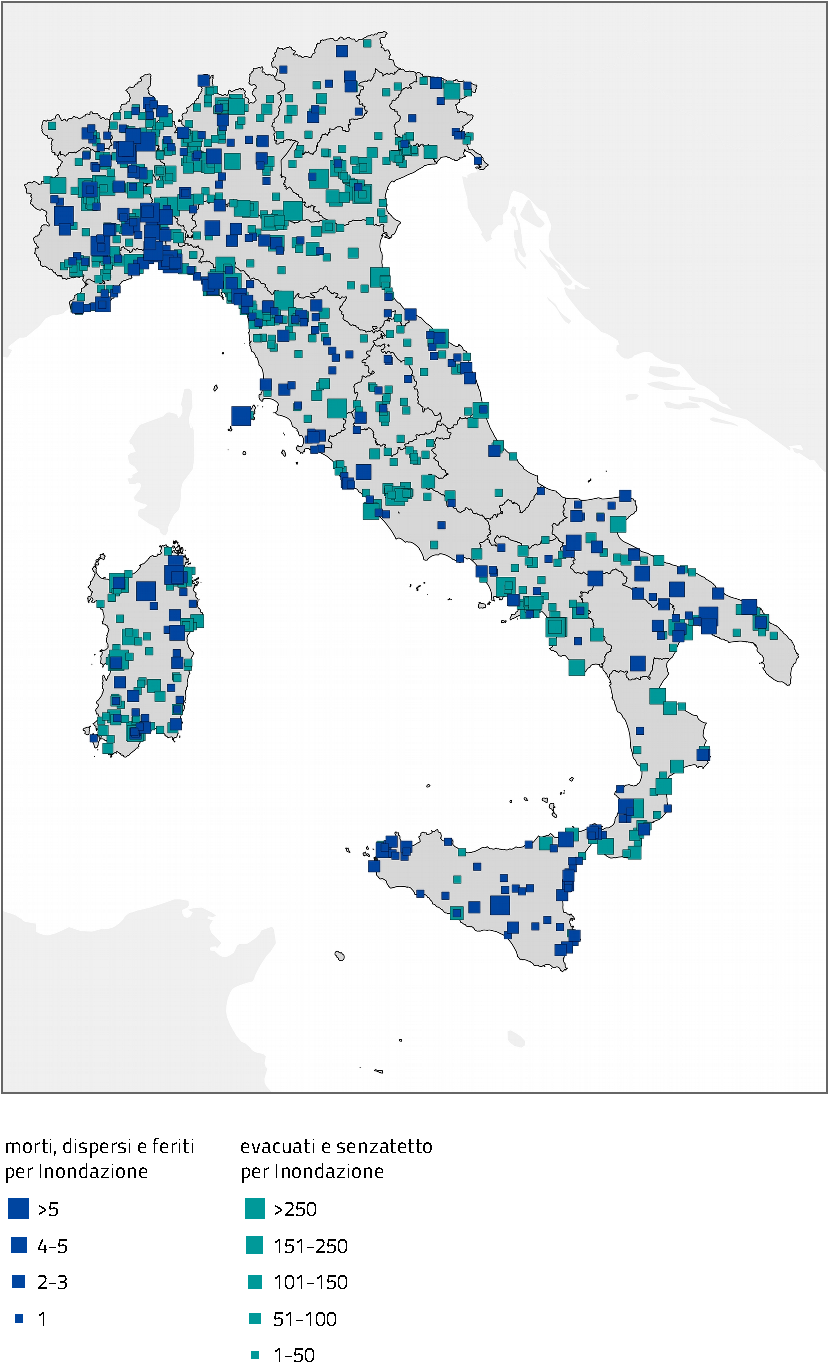
\includegraphics[width=0.9\textwidth]{figures/ita_flood/flood_ita_people_1967-2016}
    \decoRule
    \caption[Human costs of floods in Italy, 1967--2016]{Map of human costs for all flood events in Italy between 1967 and 2016. In dark blue are deaths, missing and injured; in light blue evacuees and homeless due to flooding events. Figure taken from \citet[][page 14]{IRPI2018}.}
    \label{fig:flood_events_ita}
\end{figure}

Despite the significant impact on the area, scientific studies concerning flood hazard estimation over the complete Italian domain are few: most works focus specifically on examining limited areas or basins \citep{Sole2008, Marchesini2016, Morelli2014, DiSalvo2017}, specific past events \citep{Marchi2010, Santo2012, Masoero2013, Amadio2013, Norbiato2007}, or target flood risk rather than hazard \citep{Salvati2010, Albano2017, Dottori2016}.

Some Italian regional protection agencies and basin authorities provide open-access flood hazard maps for their specific basin of interest. The Po River Basin Authority (AdbPo), for example, provides flood hazard maps for the whole Po basin (\cref{fig:flood_po}). These maps, however, have a few limitations for scientific work: they are rarely provided with accompanying vector data, the methodology is generally undisclosed, and maps from neighbouring agencies often do not agree with each other. Additionally, maps are often provided in numerous, separated image files with small extents, such as the maps provided by the Tevere River Basin Authority (ABTevere), which are comprised of 100 extremely small areas (\cref{fig:flood_tevere_union}). This fragmentation, while useful for small-scale studies, makes large-scale analysis much more difficult.

\begin{figure}
    \centering
    \includegraphics[width=\textwidth]{figures/ita_flood/po}
    \decoRule
    \caption[Flood hazard for the Po River Basin]{Flood hazard for the Po River Basin, as estimated by the Po River Basin Authority (AdbPo) (\url{http://www.adbpo.gov.it/}). Dark blue represents high flood hazard, with Return Period 10--20 years; medium blue 100--200 years; light blue 500 years. Open waters are in muted blue.}
    \label{fig:flood_po}
\end{figure}
\begin{figure}
    \centering
    \includegraphics[width=0.5\textwidth]{figures/ita_flood/flood_tevere_union}
    \decoRule
    \caption[Union view of ABTevere flood map extents]{
    Union view of all 100 flood map extents provided by the Tevere River Basin Authority.
    From \url{http://www.abtevere.it}.
    }
    \label{fig:flood_tevere_union}
\end{figure}

A national, complete, and scientifically-based homogenised flood hazard map over Italy does not exist. The only nation-wide flood hazard product available is the report \textit{Dissesto idrogeologico in Italia: pericolosità e indicatori di rischio} \citep{ISPRA2018} from ISPRA, the Italian Superior Institute for the Ambient Protection and Research, in which the data from the single local agencies (often computed using undisclosed techniques) is merged and provided as vector data. Fluvial floods and storm surges are both considered, but no distinction is made in the output product.\\ \Cref{fig:ispra_ita_flood/a,fig:ispra_ita_flood/b,fig:ispra_ita_flood/c} show the ISPRA maps for high, medium and low hazard. The most affected areas are the Romagna, Valle D'Aosta, Piedmont, Lombardy and Tuscany regions, while the hazard is significantly lower towards the South and North-East of Italy. It is hard to discern whether regional differences (such as the increased risk in Valle D'Aosta compared to the neighbouring Piedmont or the relatively low hazard in the North-Eastern regions) come from real physical and meteorological diversities or from discrepancies in methodology and underlying data. \Cref{fig:ispra_ita_flood/d} shows the population count under a medium hazard category, grouped by municipality. Neighbourhoods of major cities, such as Turin, Milan, Venice and Rome, concentrate a large number of people in areas at risk of flooding, highlighting the importance, in these areas, of suitable emergency procedures and plans based on reliable data.
\begin{figure}
    \centering
    \begin{subfigure}{.475\textwidth}
        \caption{}\label{fig:ispra_ita_flood/a}
        \includegraphics[width=\textwidth]{figures/ita_flood/p3}
    \end{subfigure}
    \begin{subfigure}{.475\textwidth}
        \caption{}\label{fig:ispra_ita_flood/b}
        \includegraphics[width=\textwidth]{figures/ita_flood/p2}
    \end{subfigure}\\
    \begin{subfigure}{.475\textwidth}
        \caption{}\label{fig:ispra_ita_flood/c}
        \includegraphics[width=\textwidth]{figures/ita_flood/p1}
    \end{subfigure}
    \begin{subfigure}{.475\textwidth}
        \caption{}\label{fig:ispra_ita_flood/d}
        \includegraphics[width=\textwidth]{figures/ita_flood/pop_p2}
    \end{subfigure}
    \decoRule
    \caption[Flood hazard in Italy according to ISPRA]{
    Flood hazard in Italy, according to \citet[][figures 2.1 to 2.3 and 4.25]{ISPRA2018}. In panel \subref{fig:ispra_ita_flood/a}, areas with low flood Return Period (high hazard, 20--50 years); in panel \subref{fig:ispra_ita_flood/b}, medium Return Period (100--200 years); in panel \subref{fig:ispra_ita_flood/c}, high Return Period (``extremely rare events''). In panel \subref{fig:ispra_ita_flood/d}, the number of people exposed to a medium hazard, by municipality. Areas where data is missing are colored in grey.
} \label{fig:ispra_ita_flood}
\end{figure}
ISPRA estimates (\cref{tab:flood_risk_ita}) 10.4\% of the population, 12.4\% of the companies, 15.3\% of the cultural heritage and 8.4\% of the surface area of Italy to be currently at medium risk of inundation (Return Period of 100 to 200 years), with higher values in the North and significantly lower hazard in the South and Isles.

\newcolumntype{M}[1]{>{\centering\arraybackslash}m{#1}}
\begin{table}[]
\begin{tabular}{@{}rrM{1.25cm}M{1.25cm}M{1.25cm}M{1.25cm}M{1.25cm}M{1.25cm}@{}}
\toprule
                                ${\rm[ \% ]}$  & Hazard & N-W & N-E & Centre & South & Islands & Whole Italy \\ \midrule
\multirow{3}{*}{Population}        & High         & 2.9        & 7.1        & 3.6    & 2.2   & 1.2     & 3.5         \\
                                   & Medium       & 5.9        & 29.1       & 10.9   & 3.9   & 1.8     & 10.4        \\
                                   & Low          & 15.1       & 28.2       & 23.5   & 5.1   & 4.3     & 15.7        \\ \\
\multirow{3}{*}{Families}          & High         & 3.0        & 7.1        & 3.5    & 2.2   & 1.2     & 3.6         \\
                                   & Medium       & 6.1        & 29.6       & 10.9   & 3.8   & 1.9     & 10.8        \\
                                   & Low          & 15.3       & 28.7       & 23.7   & 5.0   & 4.4     & 16.3        \\ \\
\multirow{3}{*}{Buildings}         & High         & 2.9        & 6.6        & 3.8    & 2.4   & 1.3     & 3.4         \\
                                   & Medium       & 5.9        & 25.8       & 10.7   & 3.4   & 2.0     & 9.3         \\
                                   & Low          & 16.0       & 25.7       & 22.1   & 4.6   & 4.2     & 14.1        \\ \\
\multirow{3}{*}{Companies}         & High         & 3.8        & 7.3        & 4.0    & 2.2   & 1.6     & 4.1         \\
                                   & Medium       & 7.1        & 29.9       & 13.2   & 4.4   & 2.4     & 12.4        \\
                                   & Low          & 16.3       & 27.7       & 28.5   & 5.8   & 5.2     & 18.4        \\ \\
\multirow{3}{*}{\parbox{2cm}{\raggedleft Cultural heritage}} & High         & 9.8        & 11.9       & 3.2    & 2.5   & 2.4     & 6.8         \\
                                   & Medium       & 14.2       & 33.7       & 8.4    & 3.3   & 3.0     & 15.3        \\
                                   & Low          & 23.7       & 34.4       & 14.0   & 4.0   & 4.8     & 19.4    \\
\bottomrule
\end{tabular}
\caption[Percentages of categories at risk of flooding]{Estimated percentage of population, families, buildings, companies and cultural heritage at three flood hazard levels, divided by Italian macroregion. High hazard corresponds to an estimated Return Period of 20--50 years; medium to 100--200 years; low to ``extremely rare events''. Macroregions are defined as follows:\\
N-W: Piedmont, Valle D'Aosta, Lombardy and Liguria; N-E: Trentino--Alto Adige, Veneto, Friuli--Venezia Giulia, Emilia--Romagna; Centre: Tuscany, Umbria, Marche, Lazio; South: Abruzzo, Molise, Campania, Puglia, Basilicata, Campania; Islands: Sicily, Sardinia.\\
Data from \citet{ISPRA2018}.}\label{tab:flood_risk_ita}
\end{table}

Although no official national study on the topic is available, in the future flood hazard is generally projected to increase in the region by several European-wide studies, in contrast with the results of some global studies (see \cref{fig:future_flood}), albeit strong differences exist among the available studies. Most works focus on estimating the change in flood hazard by focusing on the intensity or recurrence time of extreme discharges, most often $Q_{100}$, the typical 100 year Return Period discharge.\\
\Citet{Rojas2012} uses an ensemble of 12 bias-corrected simulations from the ENSEMBLES project to drive a single calibrated hydrological model (LISFLOOD) over all of Europe. Due to the large spatial extent, the study resolution is relatively low (\SI{5}{\kilo \metre}), thus reproducing only major rivers, which are not necessarily those contributing the most to flood hazard.
The results (\cref{fig:rojas_change}) generally indicate an increase in 100 year Return Period peak discharges (and thus flood intensity) under a climate change scenario (SRES A1B), when comparing the future (2071--2100) to the control period (1961--1990).
The change is, however, strongly dependent on the model and the region of interest.
In Italy, the rivers showing the greatest increase (and agreement between the 12 simulations) are those located in the North and fed by the Alpine range; changes in the Centre and South (both positive and negative) show lower agreement between models.\\
In a similar study, \citet{Thober2018} employs a multi-model ensemble of three hydrological models forced by five Global Climate Models under three different warming levels (1.5, 2 and \SI{3}{\celsius}). The climate change results are generally in agreement with \citep{Rojas2012} (despite some differences, especially in Scandinavia and the Baltic Republics), finding reduced flood hazard for Eastern Europe and Mediterranean regions, but increased hazard for North Italy (\cref{fig:thober_change}).\\
\citet{Feyen2012, Dankers2009} show more conflicting results for Italy, with only the Po river seemingly subject to increased extreme peak discharges. In some studies \citep{Roudier2016, Donnelly2017, Alfieri2015, Alfieri2015a}, on the other hand, a more uniform increase in high runoff events all over Western and Southern Europe and the Mediterranean is found (see e.g.\ figures \ref{fig:donnelly_change} and \ref{fig:alfieri_change}). In these studies, the whole Italian territory shows a marked increase in flood-related variables, although the change in the Northern basins remains more evident.

The spatial (usually \SI{5}{\kilo\meter}) and temporal (daily) resolution of the cited works is generally too low to capture the details of smaller river basins: the maps reported in these studies in fact only show major rivers in Italy. In this thesis work, which focuses only on the Italian domain, higher resolutions are possible while keeping the computational costs reasonable.

\begin{figure}
    \centering
    \begin{subfigure}{\textwidth}
        \caption{}\label{fig:rojas_change/a}
        \includegraphics[width=\textwidth]{figures/ita_flood/rojas2_crop}
    \end{subfigure}\\
    \begin{subfigure}{\textwidth}
        \caption{}\label{fig:rojas_change/b}
        \includegraphics[width=\textwidth]{figures/ita_flood/rojas3_crop}
    \end{subfigure}
    \decoRule
    \caption[Extreme discharge change in Europe according to \citet{Rojas2012}]{
    Change in extreme discharge ($Q_{100}$: peak annual discharge with 100 year Return Period), extracted from \citet[][figures 5 and 6]{Rojas2012}. In the upper panels, the number of models agreeing in a decrease (left) or increase (right) in $Q_{100}$ discharges by the end of the century, compared to the control period. In the lower panels, ensemble average of the change (left) and p-value of the signal (right).
} \label{fig:rojas_change}
\end{figure}

\begin{figure}
    \centering
    \includegraphics[width=\textwidth]{figures/ita_flood/thober}
    \decoRule
    \caption[High runoff change in Europe according to \citet{Thober2018}]{
        Change in high runoff (mean annual maximum runoff), extracted from \citet[][figure  1]{Thober2018}. The three columns represent the three warming targets considered: +\SI{1.5}{\celsius}, +\SI{2}{\celsius} and  +\SI{3}{\celsius}. In the top panel, the relative change compared to the reference period (1971--2000) and, in brackets, the spatial average. In the bottom panel, the percentage of ensemble members indicating robust changes and, in brackets, the area exhibiting changes with likelyhood greater than 66\%.
    }
    \label{fig:thober_change}
\end{figure}

\begin{figure}
    \centering
    \includegraphics[width=\textwidth]{figures/ita_flood/alfieri2015_crop}
    \decoRule
    \caption[Extreme discharge change in Europe according to \citet{Alfieri2015a}]{
        Extreme discharge ($Q_{100}$: peak annual discharge with 100 year Return Period), extracted from \citet[][figure  6]{Alfieri2015a}. In the left panel, ensemble mean of the reference period (1976--2005); in the right panel, percentage change for the time slice  2066--2095.
    }
    \label{fig:alfieri_change}
\end{figure}

\begin{figure}
    \centering
    \includegraphics[width=\textwidth]{figures/ita_flood/donnelly}
    \decoRule
    \caption[High runoff change in Europe according to \citet{Donnelly2017}]{
        Change in high runoff (mean annual maximum runoff), extracted from \citet[][figure  4]{Donnelly2017}. The four columns represent the four warming scenarios considered: +\SI{1.5}{\celsius} with RCP 2.6 and 4.5, +\SI{2}{\celsius} with RCP 2.6 and 4.5, +\SI{2}{\celsius} with RCP 4.5 and 8.5, +\SI{3}{\celsius} with RCP 4.5 and 8.5.
    }
    \label{fig:donnelly_change}
\end{figure}


%------------------------------------
%	TODO STUFF
%------------------------------------
% \section{Additional sources to integrate in this chapter}
% \begin{itemize}
% \item check all TODOs
% \item read again \url{http://ec.europa.eu/environment/water/flood_risk/flood_atlas/pdf/handbook_goodpractice.pdf}
% \item include citation EU Floods Directive (2007/60/EC) , \cite{Mysiak2013, EUFD2007}
% \item section to talk about uncertainties? \citet{alfieri2014} has a good section about it
% \item Alps are the water tower of the Po plain, and for this reason I might want to give them a closer look. I could cite one of the many kotlarski works, or e.g. \citet[][]{Gobiet2014}. View the 'Alps' category in my Mendeley, it contains about 30 works on the subject
% \end{itemize}
\chapter{Observational data}\label{chp:obs}
The main observational data used within this thesis are of four different kinds: precipitation, discharge, flood extent and terrain elevation. Due to the different peculiarities of each variable, they are treated separately in the following sections. \Cref{sec:pr_obs} will give an overview of precipitation datasets available over the study domain, including a brief analysis of precipitation uncertainty employing eight different datasets (\cref{sec:uncertainty_pr}). \Cref{sec:disch_obs,sec:flood_obs} will describe the available discharge and flood observations, while in \cref{sec:DEM} the choice of Digital Elevation Model for the subsequent hydrological and hydraulical simulations will be discussed.

%------------------------------------
%	PRECIPITATION OBS
%------------------------------------
\section{Precipitation observations} \label{sec:pr_obs}
Precipitation is probably the most difficult of all atmospheric climate variables to measure reliably, due to the huge spatio-temporal variability (especially in summer) and to the physical difficulty of setting up and maintaining a dense network of high-maintenance sensors. In our multi-model approach (see \cref{sec:3_mod_apprach}), however, it is vital that the precipitation input data is of sufficient quality and resolution to provide information even about very local, fast thunderstorms, which can trigger flooding in smaller catchments. Moreover, it is important to analyse the longest time series possible, so that rare events, which by definition have a long Return Period, can be properly represented.

In this project, precipitation observations are utilised for calibration, for validation and for driving the hydrological model CHyM (see \cref{sec:chym}).
  
\subsection{Types of precipitation measurements} \label{sec:types_pr_meas}
Precipitation measurements come from essentially three distinct sources:
\begin{description}
    \item[In-situ] Station observations are widely regarded to be the most reliable source of information for precipitation observations \citep{Hughes2006}. Several types of rain gauges exist, with the most common type of instrument being the \emph{tipping bucket rain gauge} (\cref{fig:tipping_bucket}). It consists of a small bucket of fixed size which fills up with precipitation and mechanically tips and empties, triggering a counting switch, every (usually) \SI{0.1}{\milli\metre} of rain. The buckets are usually heated, so that solid precipitation (snow, ice) is melted and correctly registered. Having moving parts means that most in-situ precipitation stations require constant and attentive maintenance, as ill-maintained sensors can easily get stuck (see \cref{fig:ts_rain/a} for an example). In general, in-situ precipitation measurements suffer greatly from the problem of gauge undercatch (see \cref{sec:gauge_undercatch}), in which, due to strong winds, a smaller amount of precipitation than expected enters the measuring funnel. In-situ data usually offer the longest time-series of all precipitation measurements techniques, with some datasets reconstructing rainfall back to the 19th century: the HISTALP project \citep{Auer2007}, for example, provides rainfall on the Alpine range using data as old as the 1800; \citep{Brunetti2006} goes as far as 1750 with monthly precipitation data over Italy. Uncertainties in in-situ data are mostly related with low station density and choice of gridding technique, so that different datasets can have significantly different climatology, especially in areas of low data availability \citep{Prein2017}. Additional details on station-based precipitation datasets, such as E-OBS and EURO4M-APGD, can be found in \cref{sec:obs_datasets}.
    \item[Ground radar] Available since the mid ’80s, ground radar observations are obtained from data on the reflectivity of the atmosphere. Rain and water vapour reflect radar waves, and the analysis of this effect allows for estimation of precipitation and wind speed; however, the displayed data can differ from the rainfall actually measured at the surface by in-situ gauges, especially in areas of complex topography, where the radio waves can easily be shielded or reflected by mountain ranges \citep{Germann2006, Wuest2010}. On the other hand, the time and space resolution of radar-based datasets cannot be matched by in-situ data. Overall, radar observations are primarily used for weather prediction and analysis and for studying specific events \citep[e.g.][]{Bertato2003}, but are sometimes also used as a tool for filling or extending other kinds of measurements.
    \item[Satellite] Space-borne precipitation measurements \citep[see][for an overview]{Kidd2011} have been available since the mid ’70s and have been on the rise in both availability and reliability ever since. Much like radars, they scan the atmosphere with several frequencies (microwave and radio), and interpret the reflected waves according to specific algorithms. Their main advantage is the relatively high resolution and very large coverage, being available even in regions where no station or radar is in place. However, the physical limitations, different measurement techniques and algorithms used to retrieve precipitation from interferometry data introduce large uncertainties \citep{Sarachi2015, Maggioni2016, Bartsotas2018, Tian2010, Bytheway2013}. Large advancements have occurred in satellite-based precipitation measurements since the early days of remote sensing from space, and there is no doubt that this data source is essential for global datasets; it is however generally found and agreed upon \citep{Rossi2017, Prein2017, Gao2013, Bowman2005} that in regions where in-situ data is available (such as most of Europe) station-based datasets still provide more reliable data. Examples of global satellite-based precipitation datasets are PERSIANN, CMORPH, TRMM, GPCP and GPM (see \cref{tab:prec_obs_ita} for citations).
\end{description}

\begin{figure}
    \centering
    \includegraphics[width=0.7\textwidth]{figures/tipping_bucket}
    \decoRule
    \caption[Tipping bucket rain gauge]{A tipping bucket rain gauge, the most common type of precipitation measuring instrument,  with the buckets exposed.}
    \label{fig:tipping_bucket}
\end{figure}

\subsection{Gauge undercatch} \label{sec:gauge_undercatch}
The main source of uncertainty for in-situ precipitation observations is the phenomenon of \emph{gauge undercatch}. This term indicates the underestimation of precipitation due to local turbulent effects around the gauge caused by the wind interacting with the sides of the instrument, as seen in \cref{fig:undercatch}. Gauge undercatch is hard to quantify, but it can severely impact the measurements of precipitation, especially for solid precipitation in windy days. According to some studies, underestimation of total precipitation can be as high as \SIrange{30}{40}{\%} for some winter stations \citep{adam2003Adjglogripresysbia, Isotta2014, Kochendorfer2017a}, with peaks of 80\% in some cases \citep{Kochendorfer2017, Wolff2015}. 
Shielded gauges, in which the collector is partially shielded from the wind (see \cref{fig:gauges}), reduce, but do not eliminate this problem \citep{Duchon2001}.\\
Correcting precipitation datasets for gauge undercatch is possible, but detailed information about local station exposure and sensor type are necessary to perform reasonable estimates \citep[see e.g.][]{Johansson2002, Mohr2009, Adler2018}.
In the Norwegian observational dataset created by \citet{Mohr2009}, for example, the correction method from \citet{Forland1996}, is applied: each station is associated with an exposure index, and a correction factor ranging from 1.02 to 1.8 (depending on precipitation type and exposure) is applied.
Observational datasets which are produced through data assimilation via a meteorological model \citep[see e.g.][]{Vidal2010, Landelius2016} often implicitly include correction factors.\\
Due to the complexity and variability of the datasets used through this thesis, and especially for the dataset described in \cref{chp:itaobs}, no attempt at correcting for gauge undercatch was performed.

\begin{figure}
    \centering
    \includegraphics[width=0.7\textwidth]{figures/undercatch}
    \decoRule
    \caption[Gauge undercatch theoretical example]{Wind velocity vectors around an unshielded gauge. Wind blowing precipitation away from the collector is the main cause of gauge undercatch. From \citet{Nespor1999}.}
    \label{fig:undercatch}
\end{figure}

\begin{figure}
    \centering
    \includegraphics[width=\textwidth]{figures/gauges}
    \decoRule
    \caption[Shielded and unshielded rain gauges]{7 different rain gauges. a) and b) are unshielded, the rest show an array of different shielding methods. From \citet{Kochendorfer2018}.}
    \label{fig:gauges}
\end{figure}

\subsection{Precipitation datasets available over Italy} \label{sec:obs_datasets}
\Cref{tab:prec_obs_ita} lists some of the currently available gridded precipitation datasets covering the Italian territory.
Two high-resolution, high-quality precipitation datasets for the Alps and Northern Italy (EURO4M-APGD and ARCIS) are available for a long observational period (38 and 55 years respectively); Central and Southern Italy, however, are only covered by European-wide and World-wide datasets, such as E-OBS, CHIRPS and the HMR reanalysis. In \cref{sec:uncertainty_pr}, a few of these datasets will be compared.\\
Of those listed in \cref{tab:prec_obs_ita}, only three high-resolution datasets provide sub-daily accumulations (PERSIANN-CDR, GPM and the UERRA reanalysis); of these, the PERSIANN-CDR reanalysis has been shown to perform poorly over Europe \citep{Prein2017}, GPM is available only since 2014, and UERRA-HARMONIE is a relatively new reanalysis which has so far seen little use and validation.
The precipitation dataset described in \cref{chp:itaobs} thus represents, to the author's knowledge, the first attempt at creating a sub-daily precipitation dataset deriving from in-situ observations specifically for the Italian territory.

% \begin{sidewaystable}[]
% \centering
% \begin{tabular}{@{}m{2.2cm}m{1.9cm}m{1.8cm}m{1.2cm}m{1.7cm}m{2.2cm}m{6cm}m{3.7cm}@{}}
% \toprule
% Name         & Region      & Period     & Spatial res.  & Time res. & Data source & Details & Reference \\ \midrule
% E-OBS        & Europe      & 1950--2017 & \ang{0.25}          & Daily     & Station data & Three step gridding process with daily anomalies over monthly field & \citet{Haylock2008} \\
% EURO4M-APGD  & Alps        & 1971--2008 & \SI{5}{\kilo\metre} & Daily     & Station data & Calculates anomalies over monthly field with PRISM, including topography & \citet{Isotta2014} \\
% HMR          & Europe      & 1979--2013 & \SI{5.5}{\kilo\metre} & Daily   & Reanalysis   & 2D Optimal Interpolation data assimilation & \citet{Landelius2016} \\
% ARCIS        & North Italy & 1961--2015 & \textasciitilde{} \SI{5}{\kilo\metre} & Daily     & Station data & Sheperd interpolation scheme with topography & \citet{Pavan2018} \\
% ISAC/CNR     & Italy       & 1961--1990 & \textasciitilde{} \SI{1}{\kilo\metre} & Monthly   & Station data & Local weighted linear regression with elevation + regional kriging & \citet{Crespi2018} \\
% UERRA-HARMONIE & Europe      & 1960--now  &\SI{11}{\kilo\metre} & Sub-daily & Reanalysis    & 3D-Var data assimilation & \citet{Ridal2017} \\
% CHIRPS       & World       & 1981--now  & \ang{0.05}          & Daily     & Station data + satellite &  & \citet{Funk2015} \\
% CPC          & World       & 1979--now  & \ang{0.5}           & Daily     & Station data & Optimal Interpolation with orography data & \citet{Chen2008a} \\
% CMORPH       & World       & 1998--now  & \ang{0.25}          & Daily     & Satellite    &  & \citet{Joyce2004} \\
% GPCC         & World       & 1901--now  & \ang{0.5}           & Monthly   & Station data &  & \citet{Schneider2014} \\
% PERSIANN-CDR & World       & 1983--now  & \ang{0.25}          & Sub-daily & Satellite    &  & \citet{Ashouri2015} \\
% TRMM-TMPA    & World       & 2000--now  & \ang{0.5}           & Daily     & Satellite    &  & \citet{Huffman2007} \\
% UDEL         & World       & 2001--2010 & \ang{0.5}           & Monthly   & Station data &  & \citet{Willmott2001} \\
% GPM          & World       & 2014--now  & \ang{0.1}           & Sub-daily & Satellite    &  & \citet{Hou2014} \\
% CRU          & World       & 1901--2016 & \ang{0.5}           & Monthly   & Station data &  & \citet{Harris2014} \\
% GPCP         & World       & 1996--2015 & \ang{1}             & Daily     & Satellite &  & \citet{Adler2018} \\ \bottomrule
% \end{tabular}\caption[List of gridded precipitation datasets over Italy]{Non comprehensive list of some gridded precipitation datasets available over Italy. At Italian latitudes, \ang{0.25} corresponds to about \SI{20}{\kilo\meter}. ***TODO*** details column}\label{tab:prec_obs_ita}
% \end{sidewaystable}

\begin{sidewaystable}[]
\centering
\begin{tabular}{@{}m{2.2cm}m{1.9cm}m{1.8cm}m{1.2cm}m{1.7cm}m{2.2cm}m{3.7cm}@{}}
\toprule
Name         & Region      & Period     & Spatial res.  & Time res. & Data source  & Reference \\ \midrule
E-OBS        & Europe      & 1950--2017 & \ang{0.25}          & Daily     & Station data & \citet{Haylock2008} \\
EURO4M-APGD  & Alps        & 1971--2008 & \SI{5}{\kilo\metre} & Daily     & Station data & \citet{Isotta2014} \\
HMR          & Europe      & 1979--2013 & \SI{5.5}{\kilo\metre} & Daily   & Reanalysis   & \citet{Landelius2016} \\
ARCIS        & North Italy & 1961--2015 & \textasciitilde{} \SI{5}{\kilo\metre} & Daily     & Station data & \citet{Pavan2018} \\
ISAC/CNR     & Italy       & 1961--1990 & \textasciitilde{} \SI{1}{\kilo\metre} & Monthly   & Station data & \citet{Crespi2018} \\
UERRA-HARMONIE & Europe      & 1960--now  &\SI{11}{\kilo\metre} & Sub-daily & Reanalysis    & \citet{Ridal2017} \\
CHIRPS       & World       & 1981--now  & \ang{0.05}          & Daily     & Station data + satellite & \citet{Funk2015} \\
CPC          & World       & 1979--now  & \ang{0.5}           & Daily     & Station data & \citet{Chen2008a} \\
CMORPH       & World       & 1998--now  & \ang{0.25}          & Daily     & Satellite    & \citet{Joyce2004} \\
GPCC         & World       & 1901--now  & \ang{0.5}           & Monthly   & Station data & \citet{Schneider2014} \\
PERSIANN-CDR & World       & 1983--now  & \ang{0.25}          & Sub-daily & Satellite    & \citet{Ashouri2015} \\
TRMM-TMPA    & World       & 2000--now  & \ang{0.5}           & Daily     & Satellite    & \citet{Huffman2007} \\
UDEL         & World       & 2001--2010 & \ang{0.5}           & Monthly   & Station data & \citet{Willmott2001} \\
GPM          & World       & 2014--now  & \ang{0.1}           & Sub-daily & Satellite    & \citet{Hou2014} \\
CRU          & World       & 1901--2016 & \ang{0.5}           & Monthly   & Station data & \citet{Harris2014} \\
GPCP         & World       & 1996--2015 & \ang{1}             & Daily     & Satellite    & \citet{Adler2018} \\ \bottomrule
\end{tabular}\caption[List of gridded precipitation datasets over Italy]{Non comprehensive list of some gridded precipitation datasets available over Italy. At Italian latitudes, \ang{0.25} corresponds to about \SI{20}{\kilo\meter}.}\label{tab:prec_obs_ita}
\end{sidewaystable}

\subsection{Uncertainty in precipitation datasets}\label{sec:uncertainty_pr}
Due to low station density, gauge undercatch and homogenisation problems, precipitation datasets can show large differences between each other. In a study utilising seven regional high-resolution datasets, two gauge-based European-wide datasets, and seven global low-resolution datasets, \citet{Prein2017} show large variability between different products, both in terms of mean and extreme precipitation; with correlations between different datasets sometimes lower than 0.5. Higher uncertainties are found, as can be expected, for extreme events and on the short-term temporal variability, while higher agreement is found on the shape of the annual cycle and on inter-annual and spatial variability.

As a brief assessment of precipitation uncertainty over Italy, in this section eight different daily precipitation datasets are compared under four different aspects: mean and extreme precipitation, precipitation distribution (probability density function) and annual cycle.
The standard $\textrm{R95}_{ptot}$ and $\textrm{R99}_{ptot}$ indexes are used to assess extreme precipitation.
They represent, for each grid point, the percentage of the total precipitation due to events higher than the 95th and 99th percentile of wet days respectively:
\begin{equation}
    \textrm{R95}_{ptot} = \frac{\sum_{PR > q95} PR}{\sum_{PR > \SI{1}{\milli\metre\per\day}} PR}\,,
\end{equation}\label{eq:r95}
where $q95$ is the 95th percentile of the daily precipitation $PR$ for wet days.\\
\Cref{tab:uncertainty_pr} lists the eight datasets used for this analysis, with their respective time period, data source and resolution; further datasets and indices to be included in this study, such as drought metrics, are being considered for the final version of this analysis \citep[][in preparation]{Fantini2018}.
Of the available datasets, only ARCIS and EURO4M-APGD have a station density that can be considered dense compared to other high-resolution regional datasets over Europe \citep[see][]{Prein2017, Fantini2016}. None of the station-based datasets considered in the analysis is gauge-corrected.
The Italian territory is split into four distinct regions: North, Centre, South and Islands, which have distinct climatic characteristics.
The analysis periods, for all datasets, start from 2000 and go up to the latest available data at the moment of this analysis.
Since different remapping procedures can impact negatively on data quality \citep{Diaconescu2015}, in order to minimise uncertainties due to data manipulation all the datasets were analysed and plotted on their own original grid.
\begin{table}[]
\centering
\begin{tabular}{@{}llll@{}}
\toprule
Dataset name & Period & Spatial res. & Data source \\ \midrule
E-OBS        & 2000--2016 & \ang{0.25}                            & Station data \\
EURO4M-APGD  & 2000--2008 & \SI{5}{\kilo\metre}                   & Station data \\
HMR          & 2000--2013 & \SI{5.5}{\kilo\metre}                 & Reanalysis \\
ARCIS        & 2000--2015 & \textasciitilde{} \SI{5}{\kilo\metre} & Station data \\
CHIRPS       & 2000--2016 & \ang{0.05}                            & Station data + satellite \\
CPC          & 2000--2016 & \ang{0.5}                             & Station data \\
CMORPH       & 2000--2016 & \ang{0.25}                            & Satellite \\
PERSIANN-CDR & 2000--2016 & \ang{0.25}                            & Satellite \\ \bottomrule
\end{tabular}
\caption[Precipitation datasets used in uncertainty analysis over Italy]{List of datasets used in the analysis of daily precipitation uncertainty carried over in \cref{sec:uncertainty_pr}. At Italian latitudes, \ang{0.25} corresponds to about \SI{20}{\kilo\meter}. See \cref{tab:prec_obs_ita} for additional details and references.}\label{tab:uncertainty_pr}
\end{table}

\Cref{fig:uncertainty_pr_mean} shows the seasonal average precipitation for the eight datasets; the extent of the four regions is highlighted in different colours in the maps.
In Northern Italy, the two datasets with the highest station density, ARCIS and EURO4M-APGD, show similar patterns and precipitation intensities.
Compared to these, the HMR reanalysis overestimates SON precipitation in the North-Eastern Alpine region, while consistently underestimating the precipitation in the Liguria region, which is an area of strong cyclogenesis and one of the most rainy in Italy.
E-OBS, while spatially coherent with the high-resolution Northern datasets, cannot resolve the same fine scale details and generally underestimates average precipitation in the Northern region.\\
In Central and Southern Italy and in the Islands, no high-density station-based dataset is available (but the one which will be presented and validated in \cref{chp:itaobs}), so the E-OBS and HMR datasets represent the benchmark against which the other datasets must perform.
Here, the CPC and CHIRPS datasets show similar patterns, with precipitation averages generally slightly above those of E-OBS, but in line with HMR.
A precipitation high point is found in Calabria in winter in HMR, CPC and CHIRPS, but less in E-OBS.
The CMORPH dataset shows particularly low precipitation in the colder months over the whole peninsula, underestimating precipitation in all seasons but JJA. PERSIANN-CDR, on the contrary, show extremely high precipitation averages across the whole period, similarly to the findings of \citet{Prein2017}.\\
The annual cycle (\cref{fig:uncertainty_pr_ac}) confirms the previous findings, with similar cycles across the four regions for E-OBS, HMR, CHIRPS, CPC, ARCIS and EURO4M-APGD, but extremely high precipitation for PERSIANN-CDR, with the opposite happening for CMORPH.
\begin{figure}
    \centering
        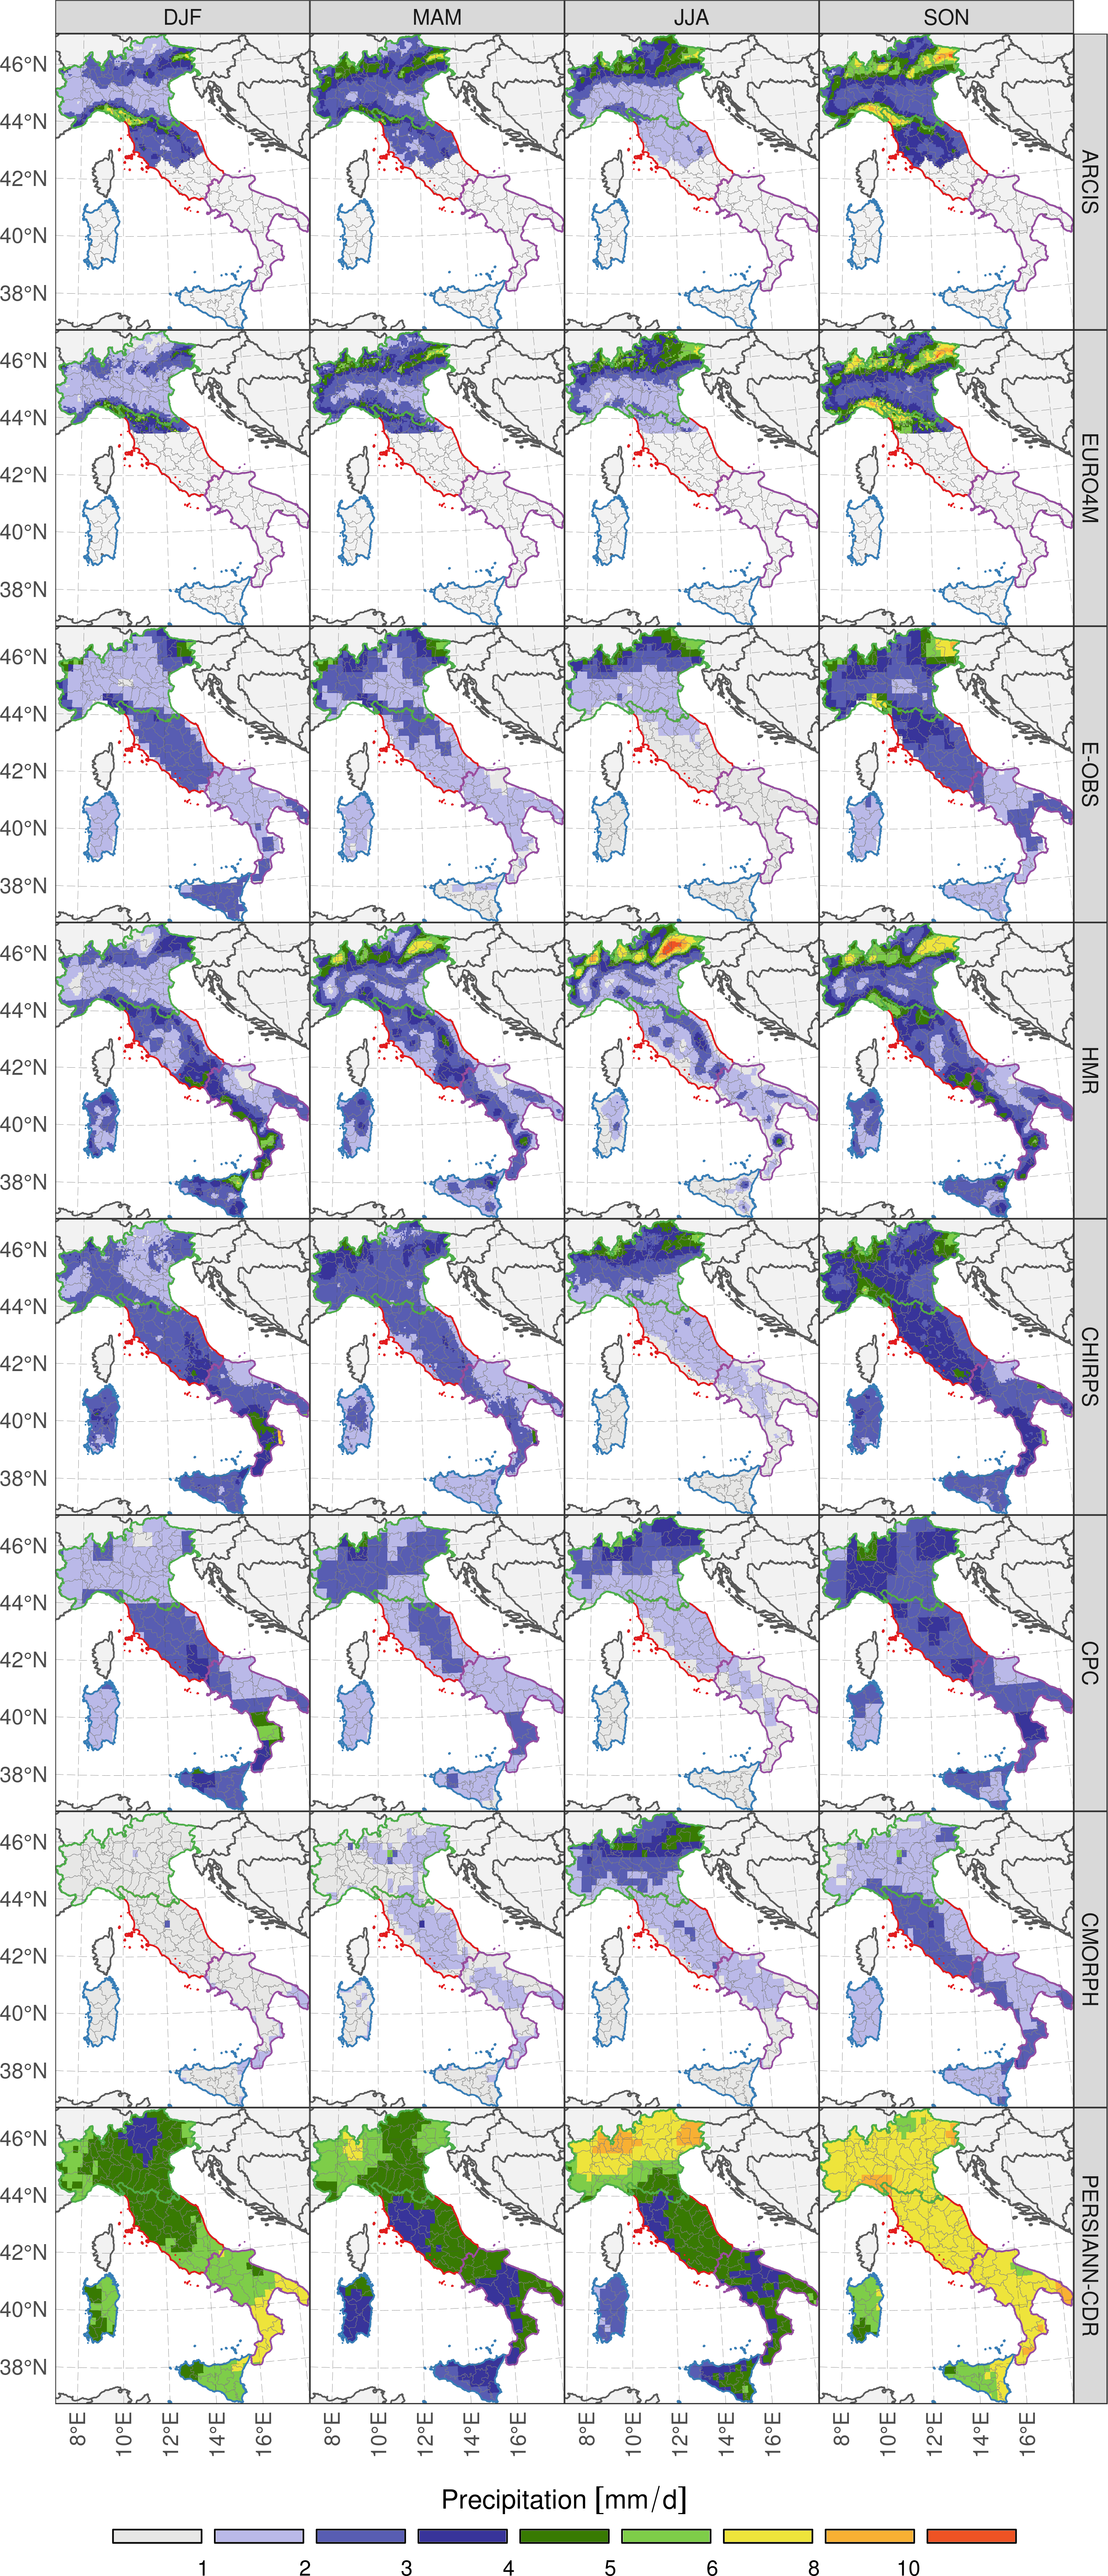
\includegraphics[width=0.7\textwidth]{figures/uncertainty/mean}
    \decoRule
    \caption[Precipitation mean: uncertainty over Italy]{
        Average precipitation for the datasets in \cref{tab:uncertainty_pr}. The four summarising regions for the annual cycle (\cref{fig:uncertainty_pr_ac}) and the PDFs (\cref{fig:uncertainty_pr_pdf1,fig:uncertainty_pr_pdf2}) are highlighted in green (North), red (Centre), purple (South) and blue (Islands).
} \label{fig:uncertainty_pr_mean}
\end{figure}
\begin{figure}
    % source of this data if you want to remake it:
    % /home/afantini/places/clima-archive4-b/regcm_simulations/EURO-CORDEX/validation/italy_validation/pr/
    \centering
        \includegraphics[width=0.7\textwidth]{figures/uncertainty/ac}
    \decoRule
    \caption[Precipitation annual cycle: uncertainty over Italy]{
        Annual cycle for average precipitation for the datasets in \cref{tab:uncertainty_pr}. The four summarising regions are highlighted in \cref{fig:uncertainty_pr_mean,fig:uncertainty_pr_r95,fig:uncertainty_pr_r99}.
} \label{fig:uncertainty_pr_ac}
\end{figure}

The spatial distribution of extreme precipitation can be assessed by \cref{fig:uncertainty_pr_r95,fig:uncertainty_pr_r99}. The three high resolution ARCIS, EURO4M-APGD and HMR datasets capture similar spatial details and amount of extremes in the North, with HMR slightly underestimating. In the other regions, large variability is present: CHIRPS almost completely lacks extremes, while CPC and PERSIANN-CDR show limited spatial variability across the regions. CMORPH, on the other hand, presents spatial patterns that are completely different from those obtained by the other products.\\
The Probability Density Functions of rainy days (\cref{fig:uncertainty_pr_pdf1,fig:uncertainty_pr_pdf2}) confirms the ability of ARCIS and HMR, in the North, to reproduce precipitation extremes not available in the other datasets. In the other regions, no clear picture seems to be discernible from the PDF data, with CHIRPS, CMORPH and HMR generally showing more intense extremes. In the South and in the Islands, E-OBS shows the least amount of extremes, while CMORPH continues to show much stronger seasonal variations compared to the other datasets.
\begin{figure}
    \centering
        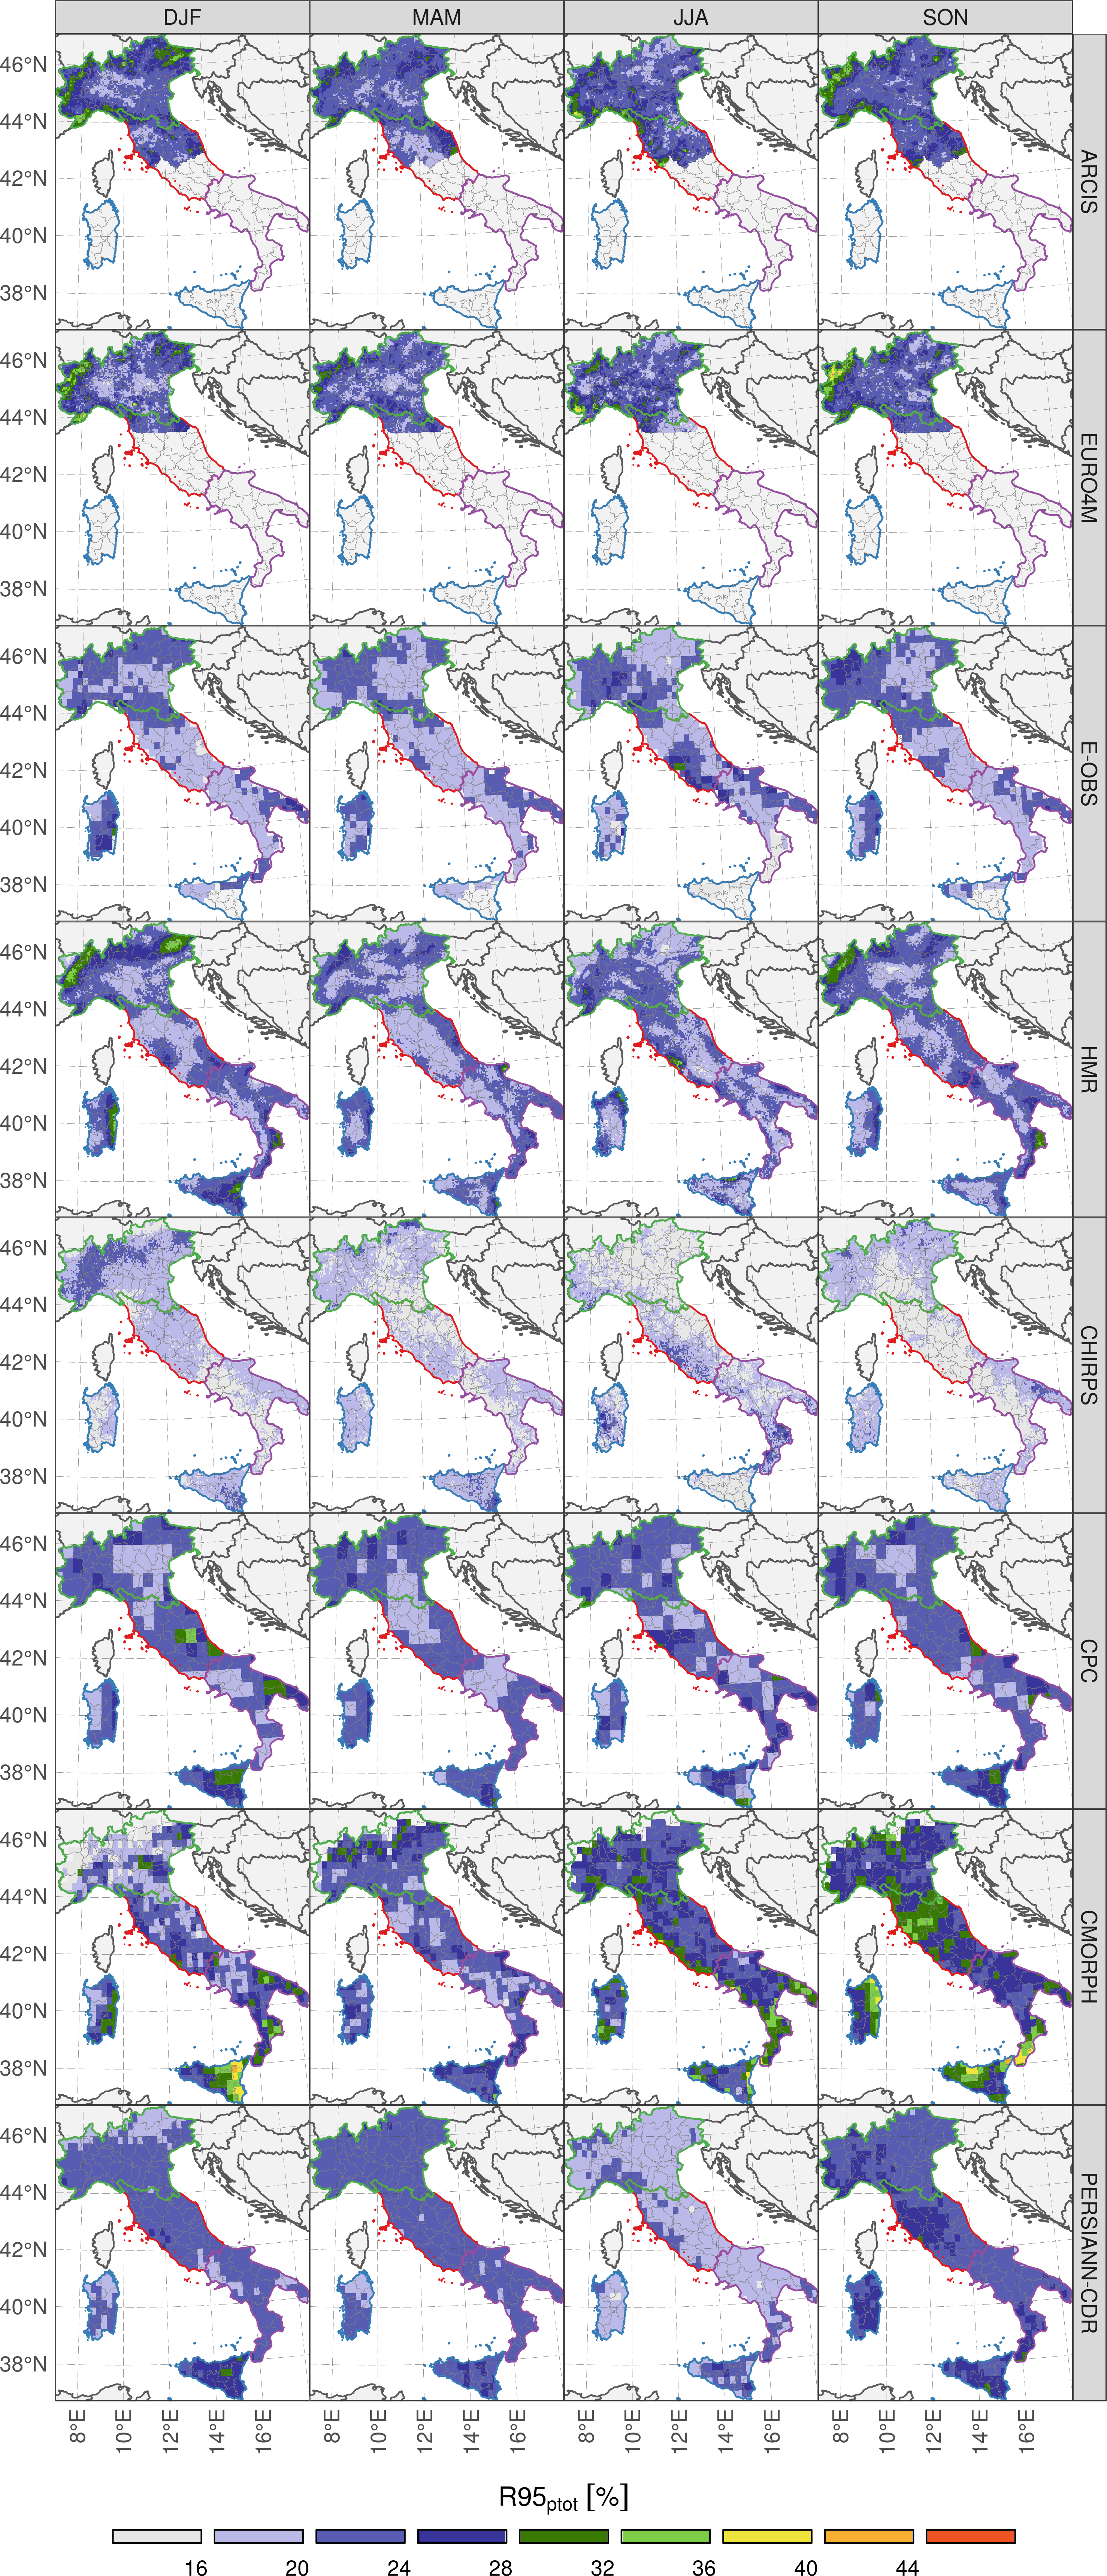
\includegraphics[width=0.7\textwidth]{figures/uncertainty/r95ptot}
    \decoRule
    \caption[Precipitation extreme ($\textrm{R95}_{ptot}$): uncertainty over Italy]{
        Extreme $\textrm{R95}_{ptot}$ precipitation for the datasets in \cref{tab:uncertainty_pr}. $\textrm{R95}_{ptot}$ represents the percentage of precipitation due to precipitation events above the 95th percentile.
} \label{fig:uncertainty_pr_r95}
\end{figure}
\begin{figure}
    \centering
        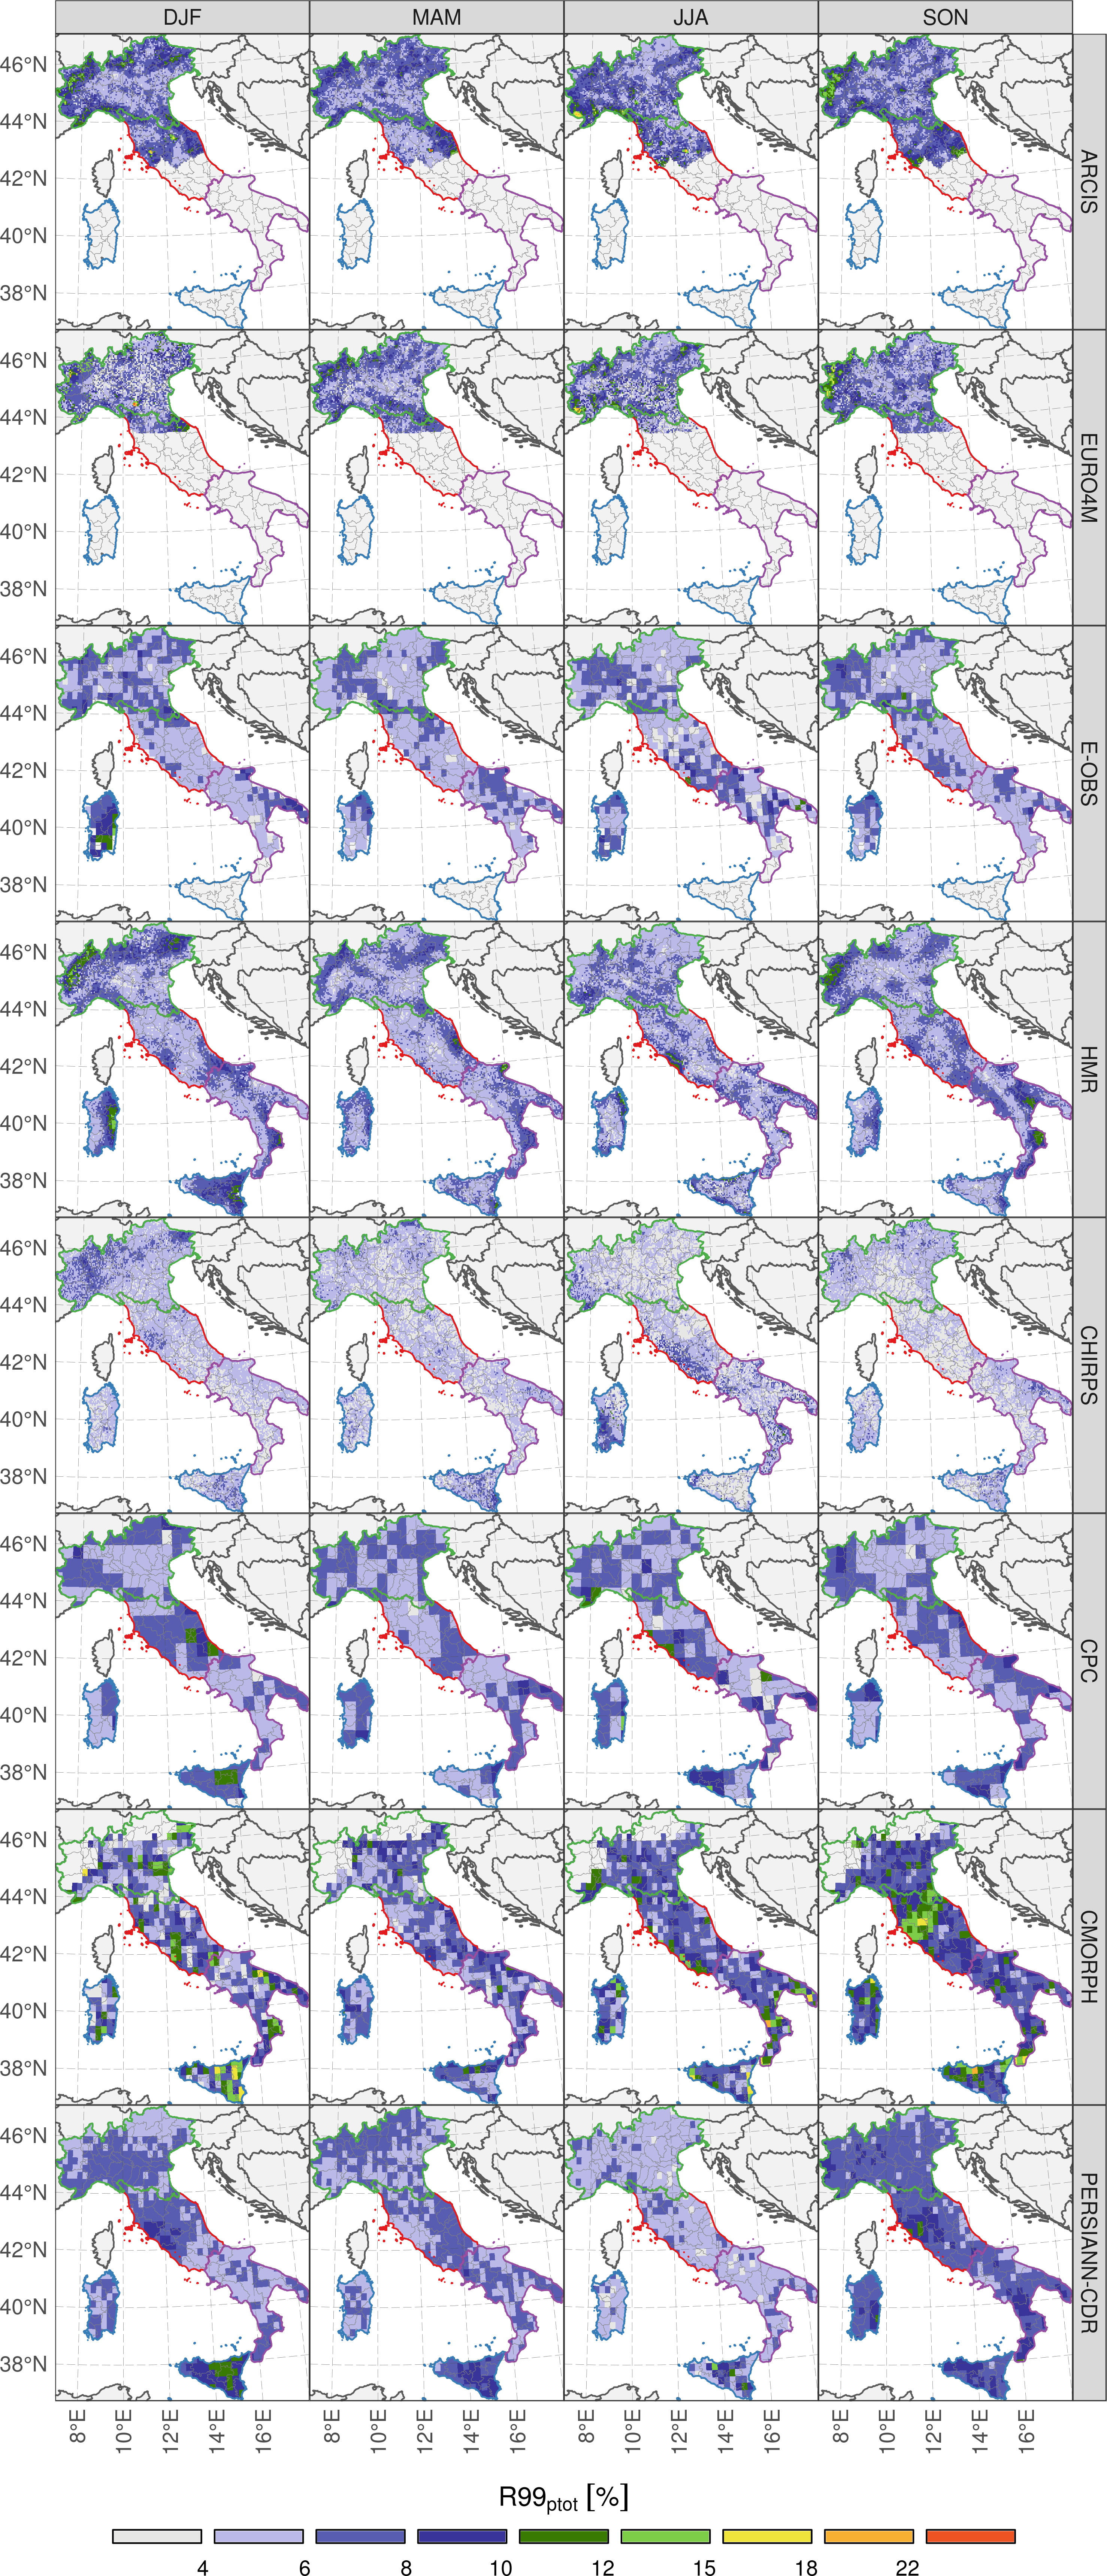
\includegraphics[width=0.7\textwidth]{figures/uncertainty/r99ptot}
    \decoRule
    \caption[Precipitation extreme ($\textrm{R99}_{ptot}$): uncertainty over Italy]{
        As \cref{fig:uncertainty_pr_r95}, but for $\textrm{R99}_{ptot}$.
} \label{fig:uncertainty_pr_r99}
\end{figure}
% \begin{figure}
%     \centering
%     \begin{subfigure}{0.8\textwidth}
% %        \caption{}\label{fig:uncertainty_pr_pdf/a}
%         \includegraphics[width=\textwidth]{figures/uncertainty/pdf_NORTH_lines}
%     \end{subfigure}\\
%     \begin{subfigure}{0.8\textwidth}
% %        \caption{}\label{fig:uncertainty_pr_pdf/b}
%         \includegraphics[width=\textwidth]{figures/uncertainty/pdf_CENTRE_lines}
%     \end{subfigure}\\
%     \begin{subfigure}{0.8\textwidth}
% %        \caption{}\label{fig:uncertainty_pr_pdf/c}
%         \includegraphics[width=\textwidth]{figures/uncertainty/pdf_SOUTH_lines}
%     \end{subfigure}\\
%     \begin{subfigure}{0.8\textwidth}
% %        \caption{}\label{fig:uncertainty_pr_pdf/d}
%         \includegraphics[width=\textwidth]{figures/uncertainty/pdf_ISLANDS_lines}
%     \end{subfigure}
%     \decoRule
%     \caption[Precipitation distribution (PDFs): uncertainty over Italy]{
%         Daily precipitation Probability Density Functions for the datasets in \cref{tab:uncertainty_pr}. The four summarising regions are highlighted in \cref{fig:uncertainty_pr_mean,fig:uncertainty_pr_r95}.
%     }\label{fig:uncertainty_pr_pdf}
% \end{figure}
\begin{sidewaysfigure}
    \centering
        \includegraphics[width=0.8\textheight]{figures/uncertainty/pdf_NORTH_lines}
        \includegraphics[width=0.8\textheight]{figures/uncertainty/pdf_CENTRE_lines}
    \caption[Precipitation distribution (PDFs): uncertainty over Italy (1)]{
        Daily precipitation Probability Density Functions for the datasets in \cref{tab:uncertainty_pr} for the North and Centre regions. The four summarising regions are highlighted in \cref{fig:uncertainty_pr_mean,fig:uncertainty_pr_r95}.
    }\label{fig:uncertainty_pr_pdf1}
\end{sidewaysfigure}
\begin{sidewaysfigure}
    \centering
        \includegraphics[width=0.8\textheight]{figures/uncertainty/pdf_SOUTH_lines}
        \includegraphics[width=0.8\textheight]{figures/uncertainty/pdf_ISLANDS_lines}
    \decoRule
    \caption[Precipitation distribution (PDFs): uncertainty over Italy (2)]{
        As \cref{fig:uncertainty_pr_pdf1}, but for the South and Islands regions.
    }\label{fig:uncertainty_pr_pdf2}
\end{sidewaysfigure}

These results show that the uncertainty associated with precipitation observations is often large, especially when it comes to precipitation extremes. In this analysis, two of the eight datasets considered (CMORPH and PERSIANN-CDR), both of which solely based on satellite data, showed very large biases (one underestimating, one overestimating) even in average precipitation, indicating that the performance of satellite-based products is insufficient in this specific region. Additionally, gauge undercatch is not taken into consideration in any of the station-based datasets employed in this brief analysis, thus uncertainty, especially for winter extreme events in mountainous regions, might be very large. On the positive side, the two Northern high-resolution datasets (EURO4M-APGD and ARCIS) show good agreement, with the HMR European reanalysis also showing good performance for mean precipitation (but a general underestimation of extremes compared to other datasets).


%------------------------------------
%	DISCHARGE OBS
%------------------------------------
\section{Discharge observations} \label{sec:disch_obs}
River discharge observations are necessary to evaluate the performance of hydrological models.
For a given river location, discharge is calculated from water level observations assuming a given \emph{stage-discharge} (or \emph{rating}) curve \citep{Braca2008}, which takes into account riverbed shape and water speed.
Stage-discharge curves are extensively used in hydrology, but they necessitate constant updates due to the fact that stream channels constantly change due to erosion, deposition of debris, vegetation growth and presence of ice.
As a consequence, despite being an irreplaceable tool, discharge measurements can sometimes be somewhat unreliable, especially for high flows \citep{DiBaldassarre2009}.\\ 
In this thesis work, datasets of discharge from several sources are considered. Similarly to the precipitation dataset exposed in \cref{chp:itaobs}, three hourly discharge datasets were provided by Prof. Marco Verdecchia\footnote{\url{http://www.dsfc.univaq.it/it/ricercatori/44-verdecchia-marco.html}}, from the University of L'Aquila; to these, the standard European Water Archive \citep{EWA2014}, containing daily data from a collection of sources over Europe, was added.
Due to the low number of daily discharge stations over Italy (only three according to the official reference\footnote{\url{ftp://ftp.bafg.de/pub/REFERATE/GRDC/website/grdc_referencestations_summary_countries.pdf}}), the Global Runoff Data Centre (GRDC) database was not selected for use in this study.
\begin{figure}
    \centering
    % source of this data if you want to remake it:
    % /home/afantini/places/clima-archive/flood/discharge_stations/dst_merge/
    \begin{subfigure}{.475\textwidth}
%        \caption{}\label{fig:disch_dst/a}
        \includegraphics[width=\textwidth]{figures/allstats_ita}
    \end{subfigure}
    \begin{subfigure}{.475\textwidth}
%        \caption{}\label{fig:disch_dst/b}
        \includegraphics[width=\textwidth]{figures/allstats_ita_2}
    \end{subfigure}
    \decoRule
    \caption[Location and time availability of the 414 discharge stations considered]{Source dataset (left) and time availability (right, in years) of the 414 discharge stations over the Italian territory, from the four datasets of \cref{tab:disc_dst}.} \label{fig:disch_dst}
\end{figure}

\Cref{tab:disc_dst} shows information about the four available datasets, while \cref{fig:disch_dst} shows the number of valid data years over Italy for each station, prior to any data checking.
The coverage of the Italian territory is not complete, with two regions (Veneto and Puglia) being completely devoid of stations, and other areas (e.g. Trentino--Alto Adige) where temporal station coverage is low, often less than five years. Some stations even have no valid data at all.
Station density and time availability are highest in Central Italy.\\
It has to be stressed that, in many cases, station locations were found to be erroneous (especially for the EWA dataset in Southern Italy); additionally, the time range with available observations varies wildly not only from dataset to dataset, but also within the same dataset.
Data quality problems, ranging from stuck sensors (see e.g. \cref{fig:stuck_disc_sensor}) to extreme outliers, are present in all datasets.\\
For these reasons, when performing data analysis and validation, care has to be taken to select only stations that have a sufficiently long time range, without any noticeable systematic error. To this end, manual controls using several metrics (among which interquartile range, standard deviation to mean ratio, frequency of most common values, number of outliers) and comparison of nearby timeseries are carried out. However, only the most conspicuous errors are guaranteed to be removed by this procedure, and many inhomogeneities and suspicious timeseries remain in the datasets.\\
Similarly to all the other data sources used in this thesis, the four discharge datasets are converted to netCDF files compliant with the CF-1.7 conventions; for additional information on the rationale and the practical advantages of using of this file format, refer to \cref{sec:netcdf}.\\

\begin{figure}
    \centering
        \includegraphics[width=\textwidth]{figures/stuck_discahrge_ts}
    \decoRule
    \caption[Example of a discharge station with a stuck sensor]{
    Example of a discharge station with a sensor stuck at \SI{351}{\cubic\metre\per\second} for almost 3 years. Some station statistics used to assess station quality are listed at the top of the figure.
} \label{fig:stuck_disc_sensor}
\end{figure}

\begin{table}[]
\centering
\begin{tabular}{@{}m{1.3cm}m{1.5cm}m{1.8cm}m{2cm}m{1.8cm}m{1.8cm}@{}}
\toprule
Dataset name & Region & Number of stations & Max period & Frequency & File type \\ \midrule
MV1 & Po river & 7 & 1995--2005 & Hourly & Fortran binary \\
MV2 & Upper Po basin & 43 & 2000--2010 & Hourly & Fortran binary \\
MV3 & Italy & 152 & 2000--2016 & Hourly & Fortran binary \\
EWA & Europe & 4058 (231 in Italy) & 1863--2013 & Daily and monthly & Plain text \\ \bottomrule
\end{tabular}
\caption[List of discharge observations]{Discharge datasets used in this thesis. See \cref{fig:disch_dst} for station locations in Italy. Datasets provided by Marco Verdecchia are named MV1 to MV3.}\label{tab:disc_dst}
\end{table}


%------------------------------------
%	FLOOD OBS
%------------------------------------
\section{Flood extent observations} \label{sec:flood_obs}
Flood extent observations are useful to validate and evaluate model performance against real world flood events.
Unfortunately, availability of precise maps of flooded areas over Italy is lacking due to the aforementioned fragmentation of regional environment agencies and lack of national coordination.
In the last decades, thanks to advancements in flood mapping techniques from satellite, by analysing Landsat, MODIS, Sentinel-1, SRTM and other remotely-retrieved data, several projects have started offering flood monitoring and maps with global or regional extent \citep[see e.g.][]{Clement2017, Schlaffer2015, Martinis2015, SMITH1997, Martinis2013, Brakenridge2003, Westerhoff2013}.\\
The Dartmouth Flood Observatory \citep[DFO,][]{G.R.Brakenridge2015}, for example, provides metadata for all major events worldwide from 1985 to present, including shapefiles indicating affected areas.
These are, however, extremely approximate and do not help in the precise identification of flooded areas (see \cref{fig:DFO_floods_ita}); additionally, only 37 events are reported in Italy in the period 1985--present, in comparison with several hundred events listed by IRPI for the period 1967--present (\cref{fig:flood_events_ita}).
\begin{figure}
    \centering
    \includegraphics[width=0.7\textwidth]{figures/ita_flood/DFO_floods_ita}
    \decoRule
    \caption[Flooded areas in the DFO database]{
        All areas in Italy affected by a flood event, as provided by the Dartmouth Flood Observatory (DFO). Areas are coloured by their DFO ID.
} \label{fig:DFO_floods_ita}
\end{figure}

The DFO also provides in-depth analysis for specific large events via the NASA-supported Global Flood Monitoring System (GFMS). \Cref{fig:DFO_flood_nov18}, for example, shows the November 2018 flooding in Northern Italy as detected by the DFO algorithms from satellite data: comparing with reported flooding by news sources, only a small part of the flooded areas in Northern Veneto and Liguria is included, and the Sicily flash flooding that caused 9 casualties is not reported at all. For comparison, the NASA NRT Global Flood Mission \citep{Nigro2014} shows even less flooding for the same period and area (\cref{fig:NRT_flood_nov18}).
\begin{figure}
    \centering
    \includegraphics[width=\textwidth]{figures/ita_flood/2018Italy4699}
    \decoRule
    \caption[Flooded area in the November 2018 Italian flood]{
        Flooded areas in Northern Italy for the November 2018 event, from the DFO archive (DFO event number 4699). Blue is reference water extent, grey is maximum water extent in the archive, and red is peak flooding for this event. Image from \url{http://floodobservatory.colorado.edu/Events/4699/2018Italy4699.html}.
} \label{fig:DFO_flood_nov18}
\end{figure}

\begin{figure}
    \centering
    \includegraphics[width=\textwidth]{figures/ita_flood/MFM_2018305_010E050N_3D3OT}
    \decoRule
    \caption[Flooded area in the November 2018 Italian flood]{
        Flooded areas (or absence thereof) in North-Eastern Italy for the November 2018 event from the MODIS NASA NRT Global Flood Mission . Image from \url{https://floodmap.modaps.eosdis.nasa.gov/getTile.php?location=010E050N&day=305&year=2018&product=3}.
} \label{fig:NRT_flood_nov18}
\end{figure}

Several challenges in flood mapping still need to be overcome in order to provide reliable flood extent dataset for all major events. For example, small rivers often cannot be mapped or are severely underestimated by satellites due to the shielding effect of vegetation \citep{SMITH1997}; algorithm details and calibration also add an additional level of uncertainty which is often difficult to quantify \citep{Stephens2012}.\\
Due to these challenges, the current focus of companies and research scientists seems to be mainly on near-real-time flood monitoring, short-term forecasting and long-term flood hazard mapping, rather than on validation of specific events. As such, few detailed observations of flood events are available over the Italian territory; tools such as the Aqueduct Global Flood Analyzer \citep{Luo2015} from the World Resources Institute, the Web Portal from DFO\footnote{\url{https://diluvium.colorado.edu/arcgis/apps/Viewer/index.html?appid=759d697577dd438ab7f2d48f605593d5}} and the Global Surface Water Explorer \citep{Pekel2016} from the European Joint Research Centre focus mainly on long-term flood hazard mapping and/or large scale events only.
The Copernicus Global Flood Awareness System \citep[GLOFAS][]{Alfieri2013}, instead, provides daily flood extents and short-term flood forecasts. The COSMO-SkyMed stellite constellation \citep{Covello2010} has been used for evaluation of specific flood events \citep[see e.g.][]{Refice2014, Pierdicca2013, Pulvirenti2011}, but the data availability seems to be limited. In short, very little information is currently available to validate inundation models against specific events over Italy: in this work, information from all of the above sources was taken into account and used when possible, given the above mentioned caveats.


%------------------------------------
%	DEM OBS
%------------------------------------
\section{Elevation observations} \label{sec:DEM}
Elevation information for each location in the study area is necessary for the hydrological (CHyM, \cref{sec:chym}) and and hydraulical (CA-2D, \cref{sec:ca2d}) models: the former uses elevation to reconstruct a realistic river network; the latter, instead, uses it to know where and how water can propagate in case of flooding. For both of these applications, high vertical accuracy, proper river routing and high horizontal resolution are necessary.

Satellite-based remote sensing techniques are the most common source of elevation data over the whole globe. Several publicly available datasets, such as SRTM, ASTER, TanDEM-X, GTOPO30 and AW3D30 use satellite sensing to infer terrain elevation and provide world coverage at resolutions ranging from \SI{30}{\metre} to \SI{1}{\kilo\metre}. Due to the nature of remote sensing via satellite, all of these datasets are affected by relatively large errors in the elevation, with vertical accuracies often of the order of several tens of meters. This makes them unsuitable for flood mapping especially of smaller basins and in flatlands.\\
A possible alternative is represented by datasets obtained by scanning the Earth's surface via LiDAR-equipped planes: these datasets, albeit very accurate, are usually very expensive for the end user (upwards of \SI{10}[\$]{\per\km\squared}), especially if a large area is required.\\
A third option for hydrologists and flood modellers is to use specifically conditioned Digital Surface Models (the term is sometimes used interchangeably with Digital Elevation Models, or DEMs) which include information on the position and depth of rivers. This is the course taken within this thesis work.

\subsection{The HydroSHEDS Digital Elevation Model}
In this thesis, the HydroSHEDS\footnote{Hydrological data and maps based on SHuttle Elevation Derivatives at multiple Scales} dataset  \citep{Lehner2008, Lehner2013} was selected to provide information not only about elevation data, but also river network and river depth. HydroSHEDS is based on different versions of NASA's 3 arc-second (about \SI{90}{\metre} at the equator) SRTM satellite-based elevation data, with several other datasets used for control and void filling. Being a DSM, and not a DTM (Digital Terrain Model), HydroSHEDS, like most satellite-only products, is affected by surface features such as buildings, major roadways and vegetation.
The DEM is hydrologically conditioned to reproduce river networks all over the globe using a mixture of automatic and manual techniques. In particular, the following algorithms are applied in order:

\begin{description}
    \item[Deepening of open water surfaces] Open waters such as lakes and oceans are deepened to insure proper flow towards them.
    \item[Weeding of coastal zone] Coastal areas are lowered to account for higher vegetation  height near the sea.
    \item[Stream burning] Major river courses are carved into the surface to ensure proper river flow. A \SI{500}{\metre} buffer is also carved around rivers to avoid sudden elevation changes and shape a smoother transition between the rivers and the surrounding areas.
    \item[Filtering] Local filtering with a $3 \times 3$ kernel size to remove high points blocking the flow path.
    \item[Molding of valley courses] Additional local algorithm to identify valley direction, using a $5 \times 5$ kernel.
    \item[Sink filling] Filling of non-natural sinks  which can impede river flow.
    \item[Carving through barriers] Final step to ensure continuous flow through natural (e.g.\ lakes) and man-made (e.g.\ dams) objects.
    \item[Second conditioning] After the barrier carving procedure, second application of the first six conditioning steps.
\end{description}

HydroSHEDS is particularly suited to the creation of a reliable river network for the CHyM model (see \cref{sec:chym_riv_net}), resulting in higher accuracy compared to the default \SI{300}{\metre} Italian DEM that comes with the model. Additionally, an advantage of using a global DEM is that it is easy to extend the flood mapping procedure to any area of the world, without the need to have any additional data requirement.\\
At the time of writing, the CHyM model is also being tested for running directly on the HydroSHEDS river network, without any further conditioning procedure as carried out by the model by default.

HydroSHEDS comes as ESRI binary \texttt{.bil} files, and was converted to appropriate formats to use with our models (NetCDF for CHyM and ASCIIgrid for CA2D) using GDAL's \texttt{gdal\_translate} tool \citep{GDAL}.

\subsection{Alternative elevation models}
Several DEMs are publicly available under no fee for research use, both for specific regions and with worldwide extent. \Cref{tab:DEMs} shows a non-comprehensive list of commonly-used DEMs, with their availability, references and maximum resolution.
\begin{sidewaystable}[]
\centering
\begin{tabular}{@{}m{2.5cm}lm{2.2cm}m{2.4cm}m{5cm}m{2.1cm}m{5cm}@{}}
\toprule
DEM name & Region & Provider & Resolution & Data source & Coordinate system & Reference \\ \midrule

PCN20 & Italy & Italian ministry for the environment & \SI{20}{\metre} & Contour lines from Italian Military Geographic Institute (IGM) cartography & UTM 32N EPSG:32632 & Provider site \footnote{\url{http://www.pcn.minambiente.it}} \\

TINITALY/01 & Italy & INGV & \SI{10}{\metre} & Mixed: satellite, cartography, LiDAR, ground data & UTM 32N EPSG:32632 & \citet{Tarquini2007, Tarquini2012} \footnote{\url{http://tinitaly.pi.ingv.it/}} \\

ASTER GDEM-2 & World & NASA & \SI{1}{arc-second} (about \SI{30}{\metre}) & Satellite & Lat-Lon EPSG:4326 & Provider site \footnote{\url{https://asterweb.jpl.nasa.gov/gdem.asp}} \\

SRTM & World  & NASA & \SI{1}{arc-second} (about \SI{30}{\metre}) & Satellite & Lat-Lon EPSG:4326 & Provider site \footnote{\url{https://www2.jpl.nasa.gov/srtm/}} \\

EU-DEM & Europe & EEA & \SI{25}{\metre} & SRTM and ASTER & EPSG:3035 ETRS89-LAEA & \citet{Bashfield2011,Jozsa2014} \footnote{\url{https://www.eea.europa.eu/data-and-maps/data/copernicus-land-monitoring-service-eu-dem}} \\

TanDEM-X & World & DLR & \SI{90}{\metre} (free version) & Satellite & Lat-Lon EPSG:4326 & \citet{Rizzoli2017}\footnote{\url{https://geoservice.dlr.de/web/dataguide/tdm90/}} \\

ALOS World 3D (AW3D30) & World & JAXA & \SI{1}{arc-second} (about \SI{30}{\metre}) & Satellite & Lat-Lon EPSG:4326 & \citet{Tadono2016, Tadono2017} \footnote{\url{https://www.eorc.jaxa.jp/ALOS/en/aw3d30/index.htm}} \\

GTOPO30 & World  & USGS & \SI{30}{arc-second} (about \SI{1}{\kilo\metre}) & Satellite & Lat-Lon EPSG:4326 & \citet{USGS1996} \footnote{\url{https://lta.cr.usgs.gov/GTOPO30}} \\

HYDRO1K & World & USGS & \SI{30}{arc-second} (about \SI{1}{\kilo\metre}) & GTOPO30, hydrologically conditioned. Flow directions and river information available & Lat-Lon EPSG:4326 & \citet{USGS1996} \footnote{\url{https://lta.cr.usgs.gov/HYDRO1K}} \\

HydroSHEDS & World  & WWF  & \SI{3}{arc-second} (about \SI{90}{\metre})   & SRTM, hydrologically conditioned. Flow directions and river information available & Lat-Lon EPSG:4326 & \citet{Lehner2008, Lehner2013} \footnote{\url{https://www.hydrosheds.org}} \\ \bottomrule
\end{tabular}\caption[List of DEMs over Italy]{Non comprehensive overview of some free-to-use DEMs and DTMs available over Italy.}\label{tab:DEMs}
\end{sidewaystable}

\begin{figure}
    %DEM difference tests: /home/clima-archive4-b/afantini/DEM/test_difference2/
    \centering
    \includegraphics[width=0.5\textwidth]{figures/DEM/PCN20.png}
    \decoRule
    \caption[Comparison of DEMs: PCN20]{
    Elevation of the Italian PCN DEM at \SI{20}{\metre} resolution; detail of a selected North-Eastern Italian region centred around the town of Belluno. Rivers (dark blue) and lakes (bright blue) are from the Interregional Centre for Information, Geographical and Statistical Systems (CISIS) DBPrior10K project\footnote{\url{http://www.centrointerregionale-gis.it/DBPrior/DBPrior.html}}.
    }
    \label{fig:PCN20}
\end{figure}
In \cref{fig:PCN20} and \ref{fig:DEMs_bias}, six of them are compared for a small ($\ang{0.3}\times\ang{0.3}$) mountainous region in North-Eastern Italy, with reference to the Italian official PCN20 \SI{20}{\metre} DEM (whose elevation is displayed in \cref{fig:PCN20}). 
The region of choice, centred around the town of Belluno, includes deep valleys, a major lake towards the East and a large river (for the standards of the region) flowing through from North towards South-West.
\Cref{tab:DEMs_stats} shows mean, standard deviation, median and 5--95\% quantile ranges for the bias with the reference dataset. Large variations of up to several tens of meters can be found between the datasets (\cref{fig:DEMs_bias}); additionally, one dataset (Nasa's SRTM) shows large no-data regions which would need to be filled in before usage with a hydrological model was possible. The conditioned version of HydroSHEDS is, on average, several meters deeper than the other datasets (\SI{18.4}{\metre} deeper than the non-conditioned version), with a 5--95\% bias quantile range of \SIrange{-86}{29}{\metre}, the widest among those considered. Carved flow paths are evident along the main course of the river and in the largest lake.

\begin{figure}
    \centering
    \includegraphics[width=\textwidth]{figures/DEM/bias_with_PCN20.pdf}
    \decoRule
    \caption[Comparison of DEMs: bias with PCN20]{
    Example comparison of 6 DEMs (see \cref{tab:DEMs}) over a small region in North-Eastern Italy centred around the town of Belluno. Elevation biases are calculated with reference to the national PCN20 DEM displayed in \cref{fig:PCN20}. Red means the DEM is higher than PCN20, green indicates the opposite. For the purpose of this example, all grids were warped to a common $300 \times 300$ $\ang{0.001}$ resolution grid using bilinear resampling. Overlaid simplified rivers (dark blue) are obtained from the Italian Superior Institute for the Ambient Protection and Research (ISPRA) online catalogue SINAnet\footnote{\url{http://www.sinanet.isprambiente.it/it/sia-ispra/download-mais/reticolo-idrografico/view}}; lakes (bright blue) are the same as \cref{fig:PCN20}.
} \label{fig:DEMs_bias}
\end{figure}

\begin{table}[]
\centering
\begin{tabular}{@{}llllll@{}}
\toprule
DEM                     & Mean   & StdDev & Q05   & Median & Q95 \\ \midrule
ASTER                   & 3.9    & 30.1   & -21   & 1      & 36 \\
HydroSHEDS Void Filled  & 0.4    & 57.8   & -52   & 0      & 51 \\
HydroSHEDS VF + Cond.  & -16.4  & 59.7   & -86   & -11    & 29 \\
JAXA AW3D30             & 5.0    & 19.6   & -14   & 3      & 26 \\
SRTM                    & 4.7    & 14.1   & -14   & 3      & 25 \\
TINITALY/01              & -0.6   & 14.1   & -19.3 & -0.6   & 17.7   
\end{tabular}
\decoRule
\caption[Comparison of DEMs: bias metrics with PCN20]{Statistics for the DEM comaparison of \cref{fig:DEMs_bias}. All values are in meters.} \label{tab:DEMs_stats}
\end{table}

In general, the choice of Digital Elevation Model must be driven by the project's requirements, and not by average bias. In this case, a reliable river network representation was paramount, leading us to settle with HydroSHEDS as terrain model of choice. Other global and regional elevation datasets were tested by attempting to reconstruct a reasonable river network via the hydrological model CHyM (\cref{sec:chym_riv_net}), but none allowed to reconstruct the rivers as well as the hydrologically conditioned HydroSHEDS.
 
\chapter{GRIPHO: developing an Italian high-resolution hourly precipitation dataset}\label{chp:itaobs}
In order to simulate flood hazard on the scale of a small catchment, high resolution precipitation data is needed. This is because the time scale for floods in small areas can be very short, due to the limited ability of small rivers to displace the large amounts of water that can fall in a relatively brief timespan.
While model output can be easily obtained for this scope, observations provide a very important tool for validation and evaluation of the methodology. Therefore, in this thesis project, observations are used to drive some of the simulations described in the next chapter.

Most observational datasets over Italy and Europe are daily (see \cref{sec:obs_datasets} and \cref{tab:prec_obs_ita}), which implies that very rapid precipitation extremes, which often occur in a few hours, are necessarily smoothed out when upscaled to a daily time scale.
Analysing these extremes on an hourly time scale has the potential to provide better results for flood hazard analysis, especially for small catchments with a short water residence time.
For this reason, one of the objectives of this thesis work was the creation of an hourly precipitation dataset that could serve as input to CETEMPS Hydrological Model \citep[CHyM,][, see \cref{sec:chym} for details]{Tomassetti2005,Coppola2006}, the hydrological model of our choice, which is designed to easily digest hourly data as input and has been doing so operationally for quite some time at the CETEMPS Center of Excellence\footnote{\url{http://cetemps.aquila.infn.it/}}.\\
We thus developed what can be considered, as far as we know, the first hourly precipitation database over Italy using exclusively in-situ precipitation data as input. The dataset is named GRIPHO (GRidded Italian Precipitation Hourly Observations).
This chapter will outline the work undergone in analysing, cleaning, gridding and validating GRIPHO. The resulting dataset is deemed of sufficient quality to be used in this project.\\
Later in the project, GRIPHO was used for driving the CHyM model simulations (\cref{sec:chym}) and to validate the RegCM simulations (\cref{sec:experiments}).

%------------------------------------
%	ORIGINAL INPUT DATA
%------------------------------------
\section{Original input data} \label{sec:original_input_data}
The first challenge when developing such a dataset is collecting the data: not always a single national agency can provide all the necessary information. Fragmentation of data sources, different input formats and different levels of quality checks are the main problems that need to be addressed. As previously mentioned, Italy lacks a national repository for meteorological data: regional agencies each have their own station network, data collection and cleaning procedures. Retrieving and homogenising all the necessary information from all regional agencies can prove to be a difficult task.
In this case, the input data are provided by the CETEMPS Center of Excellence of the University of L'Aquila, as part of an agreement with the International Centre for Theoretical Physics.
The dataset is the result of integration between different data sources; observations from 3712 precipitation stations located in all of Italy over the period from 2001 to 2016 are collected, validated and filtrated by different algorithms and then provided as a collection of yearly time series.
Using this input data, a gridded hourly dataset was created and validated.

The input data is provided as yearly Fortran-style binary files. The time step is quarter-hourly, and the unit of measure reportedly \SI{}{\milli\metre\per\hour}. A single, separate metadata text file contains the following fields for each station:
\begin{itemize}
    \item Station number [int]
    \item Station name [char]
    \item Province [char]
    \item Municipality [char]
    \item Latitude [dbl]
    \item Longitude [dbl]
\end{itemize}
No information on station type, height, exposure or any other metadata is provided.
Due to the severe lack of metadata, correcting for gauge undercatch (see \cref{sec:gauge_undercatch}) is deemed too complex for the scope of this project.\\
Any value less than 0 is considered to be a filling value (most often, this is the case with -10, -999 and -9999).
The total size of the input database is about \SI{3.9}{\giga B} for the period 2001 to 2016.
In absence of any additional information, the first timestep of each yearly file is assumed to be at time January 1, 00:00:00 UTC, with the following timesteps separated by 15 minutes each.

\subsection{Conversion to NetCDF}\label{sec:netcdf}
The first step for making use of this data is the conversion to a more user-friendly format. NetCDF\footnote{\url{https://www.unidata.ucar.edu/software/netcdf/}} is chosen primarily due to its widespread use across all fields of climate science and to its ease of use and metadata integration. All modern programming languages offer one or more interfaces capable of reading self-describing NetCDF data. Additionally, NetCDF offers advanced options such as transparent compression and chunking, which can speed up reading and writing significantly. The latter, chunking, is a netCDF-4 feature which allows to tune a dataset for faster access along a specific dimension: this allows for two versions of the dataset to be created as separate files, one that assures very fast reads for the complete time-series of one single station, and one that optimised the reading of all station values for a single time-step. The industry-standard CF conventions \citep{Eaton2009} version 1.7 are followed for the storing of metadata inside the files, the total size of which resulted to be around \SI{650}{\mega B}.

\subsection{Station spatial and temporal availability}
\Cref{fig:stat_pos} shows the station distribution over the study area. The coverage of the Italian territory is very complete, with an average density of one station per $9\times9$ \si{\kilo\metre\squared}, which is on par with most European high resolution observational datasets \citep[see \cref{sec:obs_datasets} and][for details]{Prein2017}. The overall spatial distribution is quite uniform over the complete Italian teritory, with generally lower density over less climatologically complex areas, such as the Po Plain.\\
\Cref{fig:stat_distr_height} shows the height distribution of the dataset, with station height values extracted from the HydroSHEDS void-filled Digital Elevation Model \citep[][also see \cref{sec:DEM}]{Lehner2008, Lehner2013} at \ang{0.00083} (about \SI{90}{\metre}) resolution, as opposed to the spatial distribution of all of the Italian territory. All elevations are well represented in the dataset, except very high elevations (above \SI{3000}{\metre}), which is to be expected due to the difficulty in setting up and maintaining such stations. Such small underrepresentation of very high elevations should not impact the precipitation field in a noticeable way.

\begin{figure}
    \centering
    \includegraphics[width=0.7\textwidth]{figures/rain_dst/stat_pos.png}
    \decoRule
    \caption[Station spatial distribution for the Italian in-situ hourly precipitation dataset GRIPHO]{Station spatial distribution for the Italian in-situ hourly precipitation dataset. All 3712 stations in the dataset are shown, regardless of their temporal availability.}
    \label{fig:stat_pos}
\end{figure}
%here might use animate package to put a gif with one timestep for each month or year, for the final PDF

\begin{figure}
    \centering
    \includegraphics[width=\textwidth]{figures/rain_dst/stat_distr_height.png}
    \decoRule
    \caption[Station height distribution for the Italian in-situ hourly  precipitation dataset GRIPHO]{Station height distribution for the Italian in-situ hourly precipitation dataset (red), compared to all of the Italian territory (blue). Bin size is \SI{120}{m}. Data from the HydroSHEDS void-filled Digital Elevation Model \citep{Lehner2008, Lehner2013}.}
    \label{fig:stat_distr_height}
\end{figure}

In \cref{fig:stat_avail_ts}, the number of available stations (stations whose value is not one of the possible NaN values) is plotted over each timestep for the whole Italian territory. Station availability grows significantly within the 16-year period, which implies that the total station density is not constant. While a variable number of stations is common for all station-based datasets \citep[see for example][, figure 2]{Haylock2008}, in this case it is particularly evident, with the actual number of active stations growing from about 500 in 2001 to about 2600 in 2012. Moreover, in some timesteps (e.g. at the beginning of 2012) the number of stations falls momentarily close to zero and little to no data is reported. In order to keep the dataset as close as possible to raw station data, in the final product these voids are not filled in with alternative datasets or via interpolation, but are rather left as missing values.

\begin{figure}
    \centering
    \includegraphics[width=0.7\textwidth]{figures/rain_dst/station_count_line.png}
    \decoRule
    \caption[Count of available stations per timestep]{Timeseries of the number of available stations for each timestep in the input data for the Italian in-situ dataset GRIPHO.} \label{fig:stat_avail_ts}
\end{figure}

Maps of the number of stations and valid timesteps per Italian region (\cref{fig:regional_stats}) show very low data availability for some regions, likely as a result of some regional agencies providing only a few years of data to the original data collector. While some regions provided 12 or even 13 years (Piemonte, Calabria) of data, one region (Sicily) only has 3 valid years in total (\cref{fig:regional_stats/b}). When taking into account the total number of timesteps and the station density  (\cref{fig:regional_stats/f}), Liguria and Friuli--Venezia Giulia come on top, with about \SI{2000}{valid values\per\kilo\metre\squared}, in contrast with Trentino--Alto Adige and Sicily, both with less than \SI{300}{values\per\kilo\metre\squared}. 

\begin{figure}
    \centering
    % source of this data if you want to remake it:
    % /home/afantini/places/clima-archive/flood/museodat2nc/interpolate_dewrain/valid_timesteps/
    \begin{subfigure}{.475\textwidth}
        \caption{}\label{fig:regional_stats/a}
        \includegraphics[width=\textwidth]{figures/rain_dst/regional_stats/plot.png}
    \end{subfigure}
    \begin{subfigure}{.475\textwidth}
        \caption{}\label{fig:regional_stats/b}
        \includegraphics[width=\textwidth]{figures/rain_dst/regional_stats/plot2.png}
    \end{subfigure}\\
    \begin{subfigure}{.475\textwidth}
        \caption{}\label{fig:regional_stats/c}
        \includegraphics[width=\textwidth]{figures/rain_dst/regional_stats/plot3.png}
    \end{subfigure}
    \begin{subfigure}{.475\textwidth}
        \caption{}\label{fig:regional_stats/d}
        \includegraphics[width=\textwidth]{figures/rain_dst/regional_stats/plot4.png}
    \end{subfigure}\\
    \begin{subfigure}{.475\textwidth}
        \caption{}\label{fig:regional_stats/e}
        \includegraphics[width=\textwidth]{figures/rain_dst/regional_stats/plot5.png}
    \end{subfigure}
    \begin{subfigure}{.475\textwidth}
        \caption{}\label{fig:regional_stats/f}
        \includegraphics[width=\textwidth]{figures/rain_dst/regional_stats/plot6.png}
    \end{subfigure}
    \decoRule
    \caption[Analysis of station availability for the Italian in-situ hourly precipitation dataset GRIPHO]{Analysis of station availability for the Italian in-situ hourly precipitation dataset GRIPHO; refer to the titles for the contents of each panel} \label{fig:regional_stats}
\end{figure}

As result of this initial analysis a large variability in the data availability is evident. Subsequent analysis (\cref{sec:data_cleaning}) confirms the lack of station coverage for some regions, especially in the early 2000s. Once again, due to the lack of suitable hourly backup data for the whole period and region, these gaps are purposefully left in GRIPHO without any attempt at filling them.

%------------------------------------
%	DATA CHECKING
%------------------------------------
\section{Data checking, flagging and cleaning} \label{sec:data_cleaning}
Due to the fragmented nature of the data, which comes from a plethora of different regional agencies, the original data provider could not guarantee that any quality control procedure or checks were performed on the station data.
As a result, understanding which eventual problems affect the input data represents the first priority in order to reduce the bias in the final product.\\ %***TODO*** add here a brief literature review on precipitation data cleaning
Several procedures are carried out in order to identify and remove errors and inconsistencies, such as:
\begin{itemize}
    \item analysing spatial and temporal distribution of the stations (\cref{fig:stat_distr_height,fig:stat_avail_ts}), also separated by region (\cref{fig:regional_stats});
    \item producing precipitation maps for each timestep and assembling into videos;
    \item manually analysing single station timeseries;
    \item automatic flagging of suspicious events in single station timeseries;
    \item automatic removal of extremely suspicious events;
    \item manual checking of monthly precipitation maps and statistics over the whole time period;
\end{itemize}
Due to the complexity of such procedure, no correction is attempted for those values that resulted to be erroneous or suspicious; additionally, no undercatch correction (see \cref{sec:gauge_undercatch}) is applied due to the lack of the sufficient station metadata.

\subsection{Station-by-station timeseries analysis and flagging}
A manual temporal analysis was carried out independently for all 3712 stations in the original dataset. During this process several inconsistencies were discovered, in particular:
\begin{itemize}
    \item the vast majority of data points are stored in round hours timesteps (timestamps ending in `:00' minutes), with only a handful values (less than 0.1\%) stored in between. This indicates that most of the data is actually hourly, and not sub-hourly.
    \item Some stations (see e.g.\ \cref{fig:ts_rain/a}) seem to suffer from issues with stuck sensors, causing constant values to be reported for very long periods of time. This occurs most often with the \SI{0}{\milli\metre\per\hour} value, but some instances of constant values differing from zero (most often values close to zero) are present.
    \item A sizeable amount of extremely high outliers (see e.g.\ \cref{fig:ts_rain/b}) was detected. Sometimes this affects only a single station in a given area, indicating a fluke or error in the instrumentation; other times several neighbouring stations appear to show the same behaviour, indicating an issue in the data collection and processing.
\end{itemize}

\begin{figure}
    \centering
    % source of this data if you want to remake it:
    % /home/clima-archive/afantini/flood/museodat2nc/dewrain_2000-2016/plots/
    \begin{subfigure}{\textwidth}
        \caption{}\label{fig:ts_rain/a}
        \includegraphics[width=\textwidth]{figures/rain_dst/63_ts.png}
    \end{subfigure}\\
    \begin{subfigure}{\textwidth}
        \caption{}\label{fig:ts_rain/b}
        \includegraphics[width=\textwidth]{figures/rain_dst/16_ts.png}
    \end{subfigure}\\
    \begin{subfigure}{\textwidth}
        \caption{}\label{fig:ts_rain/c}
        \includegraphics[width=\textwidth]{figures/rain_dst/613_ts.png}
    \end{subfigure}
    \decoRule
    \caption[Example precipitation timeseries from station data]{Three example precipitation timeseries from stations located in (top to bottom) Arienzo (Naples), Ala di Stura (Turin) and Maiori (Salerno). In panel \subref{fig:ts_rain/a}, the continuous zero values in 2003 indicate a stuck sensor. In panel \subref{fig:ts_rain/b}, a clear outlier at the end of 2005 can be considered an instrumental fluke with high certainty, due to the extremely high value above historical records. Panel \subref{fig:ts_rain/c} instead shows a station remarkable for its consistency and quality. Tables with some of the statistics computed for each station are also shown at the top of each panel.} \label{fig:ts_rain}
\end{figure}

To mitigate these problems, a multi-step approach of manual checking, driven by different metrics, is devised, comprising of \ref*{enum:steps_last} different steps:
\begin{enumerate}
    \item Flagging of suspicious events using several metrics obtained from the literature \citep{WMO2008}. The description of the metrics can be found in \cref{tab:flags_descr}. \label{enum:steps_1}
    \item Identification of values above the historical maxima for the region of interest, which are considered erroneous and removed. Three different thresholds are used, one for hourly values (\SI{200}{\milli\metre\per\hour}), one for monthly sums (\SI{1800}{\milli\metre\per\month}), and one for extreme step changes with the previous/next timestep (\SI{100}{\milli\metre\per\hour}). If these thresholds are exceeded more than 100 times in any given year, the entire year is removed. This filtering are carried out by the data provider, Marco Verdecchia, on the original binary data. \label{enum:steps_2}
    \item Second flagging of the values identical to step \ref{enum:steps_1}, to verify changes after the filtering occurred in \ref{enum:steps_2}. The results, shown in \cref{tab:flags_res}, show that the vast majority of suspicious values are removed after the initial cleaning procedure. In particular, 99.7\% of precipitation events above \SI{100}{\milli\meter\per\hour} are found to be unrealistic; the reduction drops to 76.3\% for events between 50 and \SI{100}{\milli\meter\per\hour}.
    In total, 82.1\% of the total flags are removed by applying this simple technique.
    \item Visualisation and selection of problematic months for each station using some of the metrics of point \cref{enum:steps_1}, aggregated on monthly scale and displayed via 192 (16 years $\times$ 12 months) interactive web maps (\cref{fig:clean_dewrain_screenshot,fig:ts_dewrain_example}), in which suspicious stations for each month are manually compared with their neighbours and, if considered unreliable, removed. \label{enum:steps_last}
    % ***TODO*** this figure should be updated with the line after the SECOND stage filtering!
\end{enumerate}
As a result of this cleaning process, the reduction in the total number of valid data points results to be modest and especially concentrated in the last few years (\cref{fig:filVSnofil_station_count_line}). A brief overview of the improvement on the data quality obtained thanks to these simple procedures will be presented in \cref{sec:valid_itaobs}.
\begin{figure}
    \centering
    \includegraphics[width=\textwidth]{figures/rain_dst/clean_dewrain_screenshot}
    \decoRule
    \caption[Manual cleaning procedure for the precipitation dataset  GRIPHO]{Example screenshot of one of the steps in the manual cleaning procedure for the hourly precipitation dataset GRIPHO. Here, for each month, stations are plotted on an interactive map coloured by their total precipitation amount. Clicking on a station pops up a timeseries plot for that station (\cref{fig:ts_dewrain_example}), so that several neighbouring stations can be easily compared; clicking the blue circle surrounding a station selects it for exclusion from the dataset.} \label{fig:clean_dewrain_screenshot}
\end{figure}
\begin{figure}
    \centering
    \includegraphics[width=\textwidth]{figures/rain_dst/ts_dewrain_example}
    \decoRule
    \caption[Example timeseries popup for the cleaning of the precipitation dataset GRIPHO]{Example precipitation timeseries for May 2012 for a station in Southern Italy. Graphs like this are used to compare neighbouring stations in the procedure of \cref{fig:clean_dewrain_screenshot}. About 360000 of these graphs were generated.} \label{fig:ts_dewrain_example}
\end{figure}

\begin{table}
\centering
\begin{tabularx}{\textwidth}{lX}
\toprule
Metric                                   &
                                         Meaning \\ \midrule
Total valid values                       &
                                         Number of values in the whole time series which are not one of the strings considered NA or negative \\
pr \textgreater{} Mean + \emph{n}SD      &
                                         Number of values greater than \emph{n} standard deviations from the mean; $n=10,15,20$\\
pr \textgreater{}  Median + \emph{n}IQR  &
                                         Number of values greater than \emph{n} interquartile ranges from the median; $n=10,15,20$   \\
100 \textgreater{}  pr \textgreater{}  50 mm/h &
                                         Number of values greater than \SI{50}{\milli\metre\per\hour}, but smaller than \SI{100}{\milli\metre\per\hour} \\
pr \textgreater{} 100 mm/h               &
                                         Number of values greater than \SI{100}{\milli\metre\per\hour} \\
\%Top \emph{n}                           &
                                         Percentage of values among the top \emph{n} most common values, excluding 0; $n=1, 5, 10$ \\
\% valid values                          &
                                         Total percentage of valid values \\
\% valid values $\neq$ 0                    &
                                         Total percentage of valid values which are not equal to 0 \\
\end{tabularx}
\decoRule
\caption[Description of all used metrics for suspicious values]{Description of all the metrics used for flagging suspicious values before and after the first automated cleaning procedure, and for selecting complete months to remove in the last manual process.}
\label{tab:flags_descr}
\end{table}

\begin{table}[]
\centering
\begin{tabular}{@{}llll@{}}
\toprule
Metric                                   & Original & Filtered & \% change \\ \midrule
Total valid values                       & 250M     & 244M     & -2,6\%    \\
Total flags                              & 324468   & 58008    & -82.1\%   \\
pr \textgreater{} Mean + 20SD              & 3240     & 2538     & -21.7\%   \\
pr \textgreater{} Median + 20IQR           & 49753    & 22519    & -54.7\%   \\
100 \textgreater{} pr \textgreater{} 50 mm/h & 21758    & 5171     & -76.3\%   \\
pr \textgreater{} 100 mm/h                 & 221822   & 711      & -99.7\%       
\end{tabular}
\decoRule
\caption[Metrics for suspicious values before and after automatic first stage filtering]{Selected metrics for suspicious values before and after automatic first stage filtering. See \cref{tab:flags_descr} for a description of all metrics.}  \label{tab:flags_res}
\end{table}

\begin{figure}
    \centering
    \includegraphics[width=\textwidth]{figures/rain_dst/filVSnofil_station_count_line}
    \decoRule
    \caption[Count of available stations per timestep, filtered and non-filtered]{Timeseries of the number of available stations for each timestep in the input data for the Italian in-situ dataset, before and after the first-stage filtering.} \label{fig:filVSnofil_station_count_line}
\end{figure}


%------------------------------------
%	GRIDDING
%------------------------------------
\section{Gridding and output format}\label{sec:gridding}
To be able to compare the precipitation data with other similar products and with models, interpolating the station point data onto a grid is a necessary step.
Our first approach to this issue uses a simple interpolation method; different techniques are currently being tested.
The upcoming sections consist of a general view of the challenges that had to be faced, and the technical choices that were consequently made, while gridding the precipitation dataset described in this chapter.

\subsection{Overview of gridding techniques}\label{sec:gridding_techniques}
The interpolation of sparse data is a vast topic, with tens of different methods available, each with its own advantages and disadvantages.
There is no general consensus on which is the best method for precipitation, which is particularly difficult to treat due to the extremely local aspect of the phenomena, both in time and in space (this is especially true in summer, when most precipitation is of convective nature).
The precipitation datasets available over Europe (including those in \cref{tab:prec_obs_ita}) use a plethora of different gridding techniques, some of which are listed in the following.\\

The de-facto standard E-OBS dataset \citep{Haylock2008} uses a three step process: daily anomalies are applied with kriging over a monthly field obtained by spatial splines, taking into account the station elevation for the monthly averages.
The high-resolution EURO4M-APGD Alpine dataset \citep{Isotta2014} opts for a similar approach with a base field calculated with an adapted PRISM method \citep{Daly1994,Schwarb2001} and daily values obtained via a modified version of the SYMAP algorithm, which is a form of inverse distance weighting \citep{Shepard1984};
this algorithm \citep[adapted by][]{Antolini2016} is also used to produce the ARCIS dataset \citep{Pavan2018}.
KLIMAGRID \citep{Mohr2008,Mohr2009} instead chooses an approach based on Delaunay triangulation, in order to minimise smoothing at station points and keep extremes intact.
The HYRAS \citep{Rauthe2013} high-resolution dataset over Germany uses the REGNIE method \citep{Weerts2008}: for each different climatological area, mean fields and climatologies are calculated using least-squares multiple linear regression (against location, slope, height and exposition) and inverse distance weighting.
The Austrian dataset SPARTACUS \citep{Hiebl2017} calculates a base field with kriging and topographic predictors, to which SYMAP daily anomalies are applied.

To our knowledge, there is limited literature comparing the performance of these interpolation methods for high-resolution gridded precipitation data. A general validation was carried over by \citet{Hofstra2008}, which ultimately resulted in the choice of interpolation technique for the E-OBS dataset mentioned above.

\subsection{The chosen spatial grid}
The choice of grid is dictated by station density and convenience. With an average station spacing of about \SI{10}{\kilo\meter}, the grid choice fell on the \SI{12}{\kilo\meter} EURO-CORDEX one used by the Regional Climate Model RegCM. The resulting $95 \times 110$ grid (\cref{fig:rain_dst_grid}) has a constant grid spacing of \SI{12}{\kilo\meter} on a Lambert Conformal Conic projection. Unlike more common regular latitude-longitude grids, using a curvilinear grid preserves constant grid cell areas, which simplifies later calculations.

\begin{figure}
    \centering
    \includegraphics[width=0.7\textwidth]{figures/rain_dst/rain_dst_grid}
    \decoRule
    \caption[Grid for the hourly rain dataset GRIPHO over Italy]{Grid of the hourly rain dataset GRIPHO over Italy, projected over Esri\copyright \ World Imagery tiles in Mercator projection (EPSG code 3857).} \label{fig:rain_dst_grid}
\end{figure}

\subsection{Gridding procedure}
In this work, due to technical constraints, a simple interpolation technique (which minimises the smoothing of extreme phenomena) is chosen to regrid the cleansed station data obtained after the manual and automatic filtering steps seen in \cref{sec:data_cleaning}\footnote{
    The regridding software was adapted for use on this project from a program provided by Graziano Giuliani from Earth System Physics (ESP) section of the International Centre for Theoretical Physics (ICTP), who also helped at various stages of this project with general software consulting. Graziano's help was irreplaceable and greatly appreciated.
}.\\ 
The method is based on SciPy's \citep{Jones2007} \texttt{interpolate.griddata}, which employs the Qhull library\footnote{\url{http://www.qhull.org}} \citep{Barber1996}. 
Both the linear and the cubic variant were taken into consideration, but since no significant climatological difference was found between the two methods, the linear version was employed.
This method performs a Delaunay triangulation \citep{Aurenhammer1991} on all the available points separately for each timestep, creating a grid of triangular cells whose corner values are linearly interpolated to evaluate the cell values on the underlying rectangular grid.
In this sense, this procedure is similar to the works of \citet{Velasquez2011,Mohr2008}, which also used Delaunay triangles to perform interpolation of sparse rainfall data sources.
An example Voronoi diagram associated to the Delaunay triangulation of the timestep containing the highest number of stations is showed in \cref{fig:voronoi}.
\begin{figure}
    \centering
    \includegraphics[width=0.7\textwidth]{figures/voronoi}
    \decoRule
    \caption[Example Voronoi diagram for the creation of the precipitation dataset GRIPHO]{Voronoi diagram corresponding to the Delaunay triangulation  of all stations. Example given for the timestep with the highest number of valid stations for the gridded Italian station-based precipitation dataset GRIPHO.} \label{fig:voronoi}
\end{figure}
After the interpolation, values over the sea are forcefully set to missing.
The result of the interpolation is, of course, more reliable for periods and regions with high station density; for this reason regions with low station density are also set to missing during the interpolation procedure.
This results in a dataset which can have both spatial and temporal empty zones, which is similar to what other station-based datasets have \citep[the E-OBS dataset from][for example, also has varying missing values]{Hofstra2008}.
The interpolation was separately carried out in parallel for each time slice, with no information crossing time boundaries.
\Cref{fig:gridVSnogrid_pdf} shows the Probability Density Function of GRIPHO in its gridded and non-gridded (raw) form: as expected, gridding introduces a general smoothing of precipitation extremes. The effect is however quite small, thanks to the choice of interpolation method, and most extreme events are retained.
Compared to most of the techniques seen in \cref{sec:gridding_techniques}, this approach is much faster but also more basic; improving this method will certainly be the goal of future research.
Additional information on the interpolation methodology, including tests with different algorithms, are presented in \citep[][in preparation]{Fantini2019a}.

\begin{figure}
    \centering
    \includegraphics[width=\textwidth]{figures/rain_dst/validation/compare.png}
    \decoRule
    \caption[PDFs for gridded and raw station data for the Italian hourly precipitation dataset GRIPHO]{Comparison of the precipitation distributions from the gridded (teal) and raw (red) hourly precipitation datasets. As is to be expected, gridding introduces a general smoothing of precipitation extremes.} \label{fig:gridVSnogrid_pdf}
\end{figure}

\subsection{Output format}
Once again, the chosen output format is CF-compliant losslessly-compressed netCDF-4. The complete GRIPHO dataset resulted in 192 monthly files, for a total of 561021 quarter-hourly timesteps over the $95 \times 110$ grid. The total size of the dataset is \SI{647}{\mega B} when adding up the sizes of each separate month, or \SI{507}{\mega B} if considering a single aggregated file; the two sizes differ because of the higher compression efficiency resulting from compressing the single, larger file. For the aggregated file, the compression ratio, when compared to an uncompressed dataset, is 44$x$.\\
Due to the aforementioned low amount of sub-hourly values an additional, hourly dataset was created by aggregating sub-hourly data. This version has 140256 timesteps and is \SI{404}{\mega B} in size.

For ease of use and download, both these versions were also further compressed by applying a lossy procedure, reducing data precision to \SI{0.1}{\milli\meter\per\hour}. In these versions, the data is stored as short (16-bit) integers, instead of 32-bit floats; a CF-standard \texttt{scale\_factor} attribute indicates these are to be rescaled to floats when read. This further reduces the size of the dataset to \SI{248}{\mega B}, or \SI{184}{\mega B} for the hourly version.

An additional GRIPHO version, containing a variable optimised for reading along the time axis, one timeseries at a time, was also produced. These multiple versions should cover all possible needs and requirements of potential users, and exceed the technical standards usually followed in producing observational datasets for climate.

%------------------------------------
%	VALIDATION
%------------------------------------
\section{Validation against other precipitation datasets}\label{sec:valid_itaobs}
In this section, the new gridded hourly precipitation product presented in this chapter is validated against some of the datasets available over the Italian territory (see \cref{sec:obs_datasets,tab:prec_obs_ita}).
Only a basic validation is presented herein, further analysis is described in detail in \citet[][in preparation]{Fantini2019a}.

\subsection{Methodology and metrics}
Due to the lack of a suitable reference hourly dataset, the validation is carried out solely on the daily scale; analysis on the hourly scale is planned as a future research path.
As reported in \cref{sec:data_cleaning}, the GRIPHO dataset had several optimisations: in the following sections GRIPHO will be analysed both in its final form and in a version obtained after the first, automated cleaning (but without the subsequent manual procedures), in order to evaluate the effectiveness of these procedures.
In the figures, this version is referred to as ``Station (interp.)''.\\
Four main metrics are presented here: annual cycle, mean seasonal precipitation, extreme seasonal precipitation ($\textrm{R95}_{ptot}$ and $\textrm{R99}_{ptot}$, see \cref{sec:uncertainty_pr}) and precipitation distribution (Probability Density Functions). Similarly to the analysis carried out in \cref{sec:uncertainty_pr}, annual cycles and PDFs are subdivided by region: North, Centre, South and Islands. Other than the product presented here, the datasets taken into consideration are EURO4M-APGD and ARCIS (only available in the North) and E-OBS and the HMR reanalysis (for the whole Italian territory). The nominal resolution of EURO4M-APGD, ARCIS and HMR is superior to that of GRIPHO. The ability to reproduce fine spatial details is however linked with station density: the EURO4M-APGD dataset, for example, is estimated to have an actual resolution of \SI{15}{\kilo\metre} or less \citep{Isotta2014}.
Similarly to \cref{sec:uncertainty_pr}, an observational period of 2000 to 2016 is considered, limited to 2008, 2013 and 2015 in the case of EURO4M-APGD, HMR and ARCIS respectively due to limited data availability.

\subsection{Results}
The annual cycle of precipitation (\cref{fig:valid_itaobs_pr_ac}) has a similar shape in all six datasets, with differences in precipitation intensity: E-OBS usually results the driest, and GRIPHO the wettest.
The filtering procedure of \cref{sec:data_cleaning} successfully removes a spurious peak in the August in the Islands, but has little to no impact on the average annual cycle of the other regions.\\
\Cref{fig:valid_itaobs_pr_mean} shows the spatial distribution of mean seasonal precipitation.
The spatial patterns and precipitation amounts in Northern Italy are remarkably similar to those from ARCIS and EURO4M-APGD.
In the other regions, GRIPHO results wetter than E-OBS and HMR, while showing similar spatial patterns with the latter.
The filtering process successfully removes some suspicious high precipitation values in Veneto (north-east, DJF) and  (centre-east, JJA), but does not filter out an excessive high value in the Southern tip of Sicily.
\begin{figure}
    % source of this data if you want to remake it:
    % /home/afantini/places/clima-archive4-b/regcm_simulations/EURO-CORDEX/validation/italy_validation/pr/
    \centering
        \includegraphics[width=0.7\textwidth]{figures/valid_itaobs/ac}
    \decoRule
    \caption[GRIPHO validation: annual cycle]{
        Average precipitation annual cycle for for the validation of the gridded hourly precipitation dataset. The four summarising regions are highlighted in \cref{fig:valid_itaobs_pr_mean,fig:valid_itaobs_pr_r95}.
} \label{fig:valid_itaobs_pr_ac}
\end{figure}
\begin{figure}
    \centering
        \includegraphics[width=0.7\textwidth]{figures/valid_itaobs/mean}
    \decoRule
    \caption[Validation of gridded hourly dataset: mean precipitation]{
        Average precipitation for the validation of the gridded hourly precipitation dataset. The four summarising regions for the annual cycle (\cref{fig:valid_itaobs_pr_ac}) and the PDFs (\cref{fig:valid_itaobs_pr_pdf1,fig:valid_itaobs_pr_pdf2}) are highlighted in green (North), red (Centre), purple (South) and blue (Islands).
} \label{fig:valid_itaobs_pr_mean}
\end{figure}

Extreme precipitation metrics (\cref{fig:valid_itaobs_pr_r95}, $\textrm{R99}_{ptot}$ not shown) once again show similar spatial patterns in the North compared with ARCIS and EURO4M-APGD and for the whole Italian region, especially compared with HMR especially.
Several extreme precipitation highs, such as the East coast of Sardinia in winter and parts of Calabria in autumn, are reproduced by both GRIPHO and HMR, but not as much by E-OBS.
The comparison of the first two rows of each plot shows that the manual filtering managed to significantly reduce what appears to be extreme precipitation excess in several areas, such as Abruzzo, Veneto, Valle d'Aosta, Sicily and Tuscany.
However, some extremes, most notably in Sicily and in Abruzzo, seem to have escaped the manual checking. For these, a second manual check will be necessary in a future version of GRIPHO.

The analysis of precipitation PDFs (\cref{fig:valid_itaobs_pr_pdf1,fig:valid_itaobs_pr_pdf2}) shows how GRIPHO contains more extreme events, compared to E-OBS and HMR, in all four regions. In the North, the difference with ARCIS and EURO4M-APGD is less striking, and all the datasets perform similarly, albeit GRIPHO seems to show some slightly more intense events than the ones in the other observational datasets.
Considering that none of these datasets include any kind of undercatch correction, this increase in extreme events is hard to evaluate.
This metric also shows very well how the filtering procedure significantly reduces the amount of extremely high precipitation events.
For the North, Centre and Isles the maximum amounts are decreased in all seasons, while no change is detected for the South of Italy.
\begin{figure}
    \centering
        \includegraphics[width=0.7\textwidth]{figures/valid_itaobs/r95ptot}
    \decoRule
    \caption[GRIPHO validation: $\textrm{R95}_{ptot}$]{
        Extreme $\textrm{R95}_{ptot}$ precipitation for the validation of the gridded hourly precipitation dataset. $\textrm{R95}_{ptot}$ represents the percentage of precipitation due to precipitation events above the 95th percentile.
} \label{fig:valid_itaobs_pr_r95}
\end{figure}
% \begin{figure}
%     \centering
%         \includegraphics[width=0.7\textwidth]{figures/valid_itaobs/r99ptot}
%     \decoRule
%     \caption[GRIPHO validation: $\textrm{R99}_{ptot}$]{
%         As \cref{fig:valid_itaobs_pr_r95}, but for $\textrm{R99}_{ptot}$.
% } \label{fig:valid_itaobs_pr_r99}
% \end{figure}
\afterpage{\clearpage}
\begin{sidewaysfigure}
    \centering
        \includegraphics[width=0.8\textheight]{figures/valid_itaobs/pdf_NORTH_lines}
        \includegraphics[width=0.8\textheight]{figures/valid_itaobs/pdf_CENTRE_lines}
    \caption[Validation of gridded hourly dataset: PDFs (1)]{
        Daily precipitation Probability Density Functions for the validation of the gridded hourly precipitation dataset for the North and Centre regions. The four summarising regions are highlighted in \cref{fig:valid_itaobs_pr_mean,fig:valid_itaobs_pr_r95}.
    }\label{fig:valid_itaobs_pr_pdf1}
\end{sidewaysfigure}
\afterpage{\clearpage}
\begin{sidewaysfigure}
    \centering
        \includegraphics[width=0.8\textheight]{figures/valid_itaobs/pdf_SOUTH_lines}
        \includegraphics[width=0.8\textheight]{figures/valid_itaobs/pdf_ISLANDS_lines}
    \decoRule
    \caption[Validation of gridded hourly dataset: PDFs (2)]{
        Daily precipitation Probability Density Functions for the validation of the gridded hourly precipitation dataset for the South and Islands regions. The four summarising regions are highlighted in \cref{fig:valid_itaobs_pr_mean,fig:valid_itaobs_pr_r95}.
    }\label{fig:valid_itaobs_pr_pdf2}
\end{sidewaysfigure}

%------------------------------------
%	SUMMARY
%------------------------------------
\section{Summary and outlook}
The hourly precipitation dataset GRIPHO represents a first of its kind for the Italian territory.
The somewhat limited time availability of the dataset (little more than 15 years) is unfortunate, but no additional data was available for before 2000.
The high spatial and temporal resolution are superior to those of E-OBS, which is still the only observation-based dataset available over the whole Italian region. Compared to the ARCIS and EURO4M-APGD datasets, which are only available in Northern Italy, the effective spatial resolution is similar, but the hourly temporal resolution is much finer.
Thanks to the high station density, reproduction of extreme events is improved, in particular if compared to E-OBS.
The  GRIPHO dataset has shown sufficient quality for it to be used to drive the hydrological model CHyM, which is at the core of this thesis work, and to validate the climate simulations performed by RegCM, as detailed in the upcoming chapters.

Availability and additional details on this dataset will be made available in an upcoming paper \citep[][in preparation]{Fantini2019a}, where
\begin{itemize}
    \item the unexpected behaviour of extreme events in Sicily and Abruzzo will be fixed by applying a further manual conditioning step;
    \item an analysis of hourly precipitation will be included;
    \item the choice of interpolation method will be discussed further;
    \item validation against further datasets available for the area only on a monthly timescale (e.g. the ISAC/CNR dataset) will be included.
\end{itemize}

\chapter{Methods and models} \label{chp:models}
The aim of this project is to evaluate flood hazard in Italy, and to project this evaluation in a possible future scenario.
In order to obtain discharge and flood information a hydrological model is used to simulate runoff over the domain.
Runoff can then be analysed statistically to provide proxies for floods (such as metrics of extreme discharge) or to drive hydraulic floodplain simulations, capable of spreading the water over the terrain and produce flood extents and water depths.\\
\Cref{fig:method} shows flow chart of the thesis work.
\begin{figure}
    \centering
    \includegraphics[width=\textwidth]{figures/method}
    \decoRule
    \caption[Flowchart of the project methodology]{A schematic description of the methodology employed in this study.}
    \label{fig:method}
\end{figure}

The precipitation data that are the main input needed to run hydrological simulations come from two different sources:
\begin{description}
    \item[High-resolution observations] the GRIPHO dataset, described in \cref{chp:itaobs}, which provide high-resolution hourly precipitation data.
    \item[Regional Climate Model simulations] two climate simulations, one run in perfect boundary mode and one with a climate projection.
\end{description}

\Cref{sec:regcm} will detail the RCM model and simulations, while \cref{sec:chym} will describe the hydrological model of choice and its three simulations.
\Cref{sec:3_mod_apprach} will delineate the statistical procedure used to derive the extreme discharge statistics from the discharge timeseries. Finally, \cref{sec:ca2d} will present the hydraulic model and its simulations.


%------------------------------------
%	REGCM
%------------------------------------

\section{The RegCM Regional Climate Model} \label{sec:regcm}
The ICTP RegCM is a Regional Climate Model developed at the ICTP and maintained primarily by Graziano Giuliani. The project is under very active development and new features, options and schemes are routinely added. RegCM is used by several institutions and research groups worldwide.\\
The RegCM model was the first limited area model to be developed for long-term climate simulations \citep{dickinson1989regional, Giorgi1989}. The model went through the second \citep{Giorgi1993}, third \citep{Pal2007} and fourth \citep{giorgi2012RegmoddespretesovemulCORdom} major revisions and is currently at version 4.7.0.\\
RegCM is a compressible, terrain-following sigma-vertical coordinate model, offering a large selection of physical parameterisations. The dynamics are essentially the same as the NCAR Mesoscale Model 4 or 5, depending on the versions and settings \citep[MM4, MM5,][]{Grell1994}.
Recently, the implementation of a non-hydrostatic core from MM5 has allowed to run in convection-permitting mode.
RegCM is mainly written in the Fortran programming language and is compliant with the Fortran 2003 ANSI standard; as most other climate models do, RegCM reads and writes files in the netCDF format.

\subsection{Regional Climate Models: an overview}
Regional Climate Models (RCMs) are Limited Area Models (LAMs) usually nested on larger datasets. RCMs are the most common tool used to ``zoom in'' on a specific area by dynamically \emph{downscaling} lower-resolution climate data. They do this by processing the information provided by the driving dataset at the domain boundaries, adding value thanks to the higher resolution and consequent more accurate representation of physical processes.\\
The first Regional Climate Models were initially developed in the late ´80s \citep{Giorgi1990, dickinson1989regional, Giorgi1989} to perform short, few-days simulations at best. In subsequent years, their use was extended to perform multi-year simulations \citep{Giorgi1993, Jones1995}. In the last two decades, several research programs utilising RCMs were put forward to advance the knowledge of climate at small spatial scales: of these, the most recent is the Coordinated Regional Climate Downscaling eXperiment (CORDEX, \cref{sec:cordex}).\\
In the nesting regional climate modelling technique, large scale (atmospheric and oceanic) time-dependent fields drive a higher resolution model over a limited domain. The driving data acts as boundary condition to the driven model and provides the initial conditions. In most cases a one-way nesting scheme is used: the nested model does not influence the boundary driving data, i.e.\ there is no feedback from the nested model to the coarser model. However, two-way coupled simulations, in which feedback from the driven model is incorporated in the boundary conditions, can be performed with some models \citep{Inatsu2009, Lorenz2005}.\\
By design, RCMs necessitate of external forcings that act as boundary conditions. These are usually of three kinds:
\begin{itemize}
    \item Model \emph{reanalysis}, such as ERA-Interim \citep{Dee2011}, are weather model simulations of the past which are constrained by a plethora of observed quantities through a complex process of data assimilation. The resulting dataset is uniform in time and space, consistent with observations, physically coherent, and provides all the necessary variables to drive an RCM. Such ``perfect boundary condition'' simulations are usually performed to validate the ability of an RCM to reproduce a reliable climate.
    \item Global Climate Models (GCMs) are physical simulations of the general circulation, much like RCMs, however with global extent and, thus, no external forcing other than the initial conditions. GCMs are the most natural choice for long climate projections; they usually have a resolution which, due to computational constraints, is significantly lower than that of RCMs.
    \item RCMs themselves can be used as driving data for even higher resolution simulations, in what is usually called a multi-nesting simulation. Such simulations are becoming more and more common thanks to the development of convection-permitting models \citep{Prein2015, Clark2016}, which often have a resolution of \SI{2}{\kilo\meter} or less and require high-resolution driving data.
\end{itemize}
Due to the presence of lateral boundary conditions, RCMs necessarily need to take into consideration  a so-called \emph{buffer zone}: a number of cells close to the domain edge in which the dynamical equilibrium between the driver and the driven model can be reached and smaller-scale features can develop. The same is true for an initial \emph{spin-up} period, usually of up to one or two years, which is excluded from analysis.

\subsection{The CORDEX project}\label{sec:cordex}
In order to properly validate whether climate models perform well, and whether RCMs add value to GCMs and reanalysis, a large number of ensemble simulations, performed on common domains, is advisable. Several  international projects have historically provided the basis for this kind of analysis. Some of these are PIRCS, START, CECILIA,
CLIM-RUN, MICE, STARDEX, PRUDENCE, SPECS, EUPORIAS, ENSEMBLES, and CORDEX. CORDEX\footnote{CORDEX stands for Coordinated Regional Climate Downscaling eXperiment} \citep{Giorgi2009, Gutowski2016, Giorgi2015}, a World Climate Research Programme (WCRP) sponsored project, is a framework for downscaling a large number of GCMs using both dynamical and statistical downscaling techniques. 14 common domains are specified (Africa, MENA, North, Central and South America, Antarctica, Arctic, EURO, MED, Australasia, East, Central, South and South-East Asia), mostly covering areas from previous intercomparison projects, with pre-defined resolutions and projections. Two European domains are defined, one covering all of the continent \citep[][EURO--CORDEX]{Jacob2014} and one focusing on the Mediterranean \citep[][Med--CORDEX]{Ruti2016}. Institutions are asked to provide data with a grid resolution of around 12, 25 or \SI{50}{\kilo \meter}; as will be shown in \cref{sec:experiments}, the domain chosen in this work covers the EURO--CORDEX area (\cref{fig:euro_cordex}) at a resolution of \SI{12}{\kilo \meter}.

\begin{figure}
    \centering
    \includegraphics[width=0.7\textwidth]{figures/eurocordex}
    \decoRule
    \caption[EURO--CORDEX domain]{The approximate EURO--CORDEX domain, from \url{http://www.cordex.org/domains/cordex-region-euro-cordex/}} \label{fig:euro_cordex}
\end{figure}

\subsection{Added value of RCMs}
Why use Regional Climate Models, when Global Climate Models are a ever-improving, tried-and-tested approach to simulating climate?
The answer is that, even with today's increasingly powerful computational resources, GCMs are still run at a resolution of several tens of kilometers: for example, the latest Coupled Model Intercomparison Project 6 \citep[CMIP6,][]{Eyring2016} includes the High Resolution Model Intercomparison Project \citep[HighResMIP,][]{Haarsma2016}, whose simulations are supposed to run with a resolution of ``at least \SI{50}{\kilo \meter}''.
By contrast, \emph{convection-permitting} RCM simulations with spatial resolutions close to that at which the hydrostatic approximation starts failing \citep[about \SI{10}{\kilo \metre}][]{giorgi1999InttospesecRegclimodrev} are not a rarity anymore \citep[e.g.][]{Prein2015, Clark2016, Coppola2018}.
Thanks to the increased resolution, the main added value of RCMs is connected with their ability to reproduce otherwise unattainable small scale features (\cref{fig:topo_av}).
This is possible because of the better representation of:
\begin{description}
    \item[Orographic forcing] Increased resolution means increased ability to represent slopes, peaks and valleys. Variables that show a pronounced elevation dependency, such as precipitation, temperature and wind speed, greatly benefit from higher ground resolution. This is especially true for complex mountain areas \citep[see e.g.][]{Giorgi1989, Fischer2014}.
    % \item[Parametrisations] Physical process parametrisation usually improves at higher resolution, thanks to smaller timesteps and pixel areas.
    \item[Direct representation of processes] Some parametrisations can be eliminated altogether at very high resolutions, opting instead for direct representation of the processes. This is the case with the already mentioned convection-permitting models, in which convection is resolved explicitly.
\end{description}
\begin{figure}
    \centering
    \begin{subfigure}{0.4\textheight}
%        \caption{}\label{fig:topo_av/a}
        \includegraphics[width=\textwidth]{figures/topo_av/EI_3d}
    \end{subfigure}\\
    \begin{subfigure}{0.4\textheight}
%        \caption{}\label{fig:topo_av/b}
        \includegraphics[width=\textwidth]{figures/topo_av/50_3d}
    \end{subfigure}\\
    \begin{subfigure}{0.4\textheight}
%        \caption{}\label{fig:topo_av/c}
        \includegraphics[width=\textwidth]{figures/topo_av/12_3d}
    \end{subfigure}
    \decoRule
    \caption[Topography representation over the Alps at different resolution]{
        Representation of topography over the Alps at different resolutions: \ang{1.50}, \ang{0.44} and \ang{0.11}, corresponding to the typical resolutions of GCMs, low-res RCMs and high-res hydrostatic RCMs respectively.
    }\label{fig:topo_av}
\end{figure}

RCMs, thus, usually add information to the global models which they are driven, if there are available observations of sufficient quality and resolution to assess this. This added information, if correct, is referred to as ``Added Value''.
It may seem obvious that increasing the resolution will improve the skill in reproducing climate.
However, added value is often hard to predict and identify, as it does not vary linearly with grid size nor is equal on different domains. As the IPCC \citep[][section 9.6.3]{IPCC2013} puts it:
\blockquote{
Although there are indications that model skill increases with higher resolution, it does not do so linearly. \citet{Rojas2006} found more improvement when increasing resolution from 135 km to 45 km than from 45 km to 15 km. \citet{Walther2013} found that the diurnal precipitation cycle and light precipitation improved more when going from 12 km to 6 km resolution than when going from 50 km to 25 km or from 25 km to 12 km. Higher resolution does enable better simulation of extremes \citep{Seneviratne2012}. For example, \citet{Pryor2012} noted that an increase in RCM resolution from 50 km to 6 km increased extreme wind speeds more than the mean wind speed. \citet{Kawazoe2013} compared six RCMs and the two GCMs to high resolution observations, concluding that precipitation extremes were more representative in the RCMs than in the GCMs. \citet{Vautard2013} found that warm extremes in Europe were generally better simulated in RCMs with 12 km resolution compared to 50 km. \citet{Kendon2012} and \citet{Chan2012} found mixed results in daily precipitation simulated at 12 km and 1.5 km resolution, although the latter had improved sub-daily features, perhaps as convection could be explicitly resolved.
}

Due to the importance of a reliable representation of extreme precipitation events for flood hazard, the added value that high resolution can provide for this variable deserves greater attention.
In a recent study, \citet{Fantini2016} compared 9 EURO-- and Med--CORDEX RCMs against high resolution regional observations for several metrics, of which two are extreme precipitation metrics.
The performance of the models was assessed at two different resolutions (\ang{0.11} and \ang{0.44}).
In most regions, the higher resolution RCMs showed better ability to reproduce extreme precipitation compared to the lower resolution ones: in the daily precipitation Probability Density Functions  (\cref{fig:added_value_pdf}), for example, the only case in which the performance was clearly degraded (when going from the \ang{0.44} to the \ang{0.11} ensemble) also coincided with the region characterised by the lowest density of stations (the Carpathians); other regions mostly showed better performance on part of the \ang{0.11} ensemble.
RCMs performed also significantly better than the driving ERA-Interim \citep{Dee2011} in all metrics (and in particular in extreme precipitation).\\
The results of this work are in general agreement, for what concerns extreme precipitation, with other similar works, such as \citet{diluca2012PotaddvalpresimbyhignesRegCliModobs, Lucas-Picher2017, Prein2016, Torma2015, Casanueva2016}, reinforcing the evidence supporting the presence of strong added value for extreme precipitation events in high-resolution RCM simulations.
\begin{figure}
    \centering
    \includegraphics[width=\textwidth]{figures/AV_PDF}
    \decoRule
    \caption[PDFs for CORDEX models, from \citet{Fantini2016}]{Probability Density Functions (PDFs) for the ensemble average of the 9 models considered in \citet{Fantini2016} over the 9 regions where high-resolution observations were available. In black, the driving ERA--Interim data; in blue and red, the \ang{0.44} and \ang{0.11} ensembles respectively; in green the regional observations.} \label{fig:added_value_pdf}
\end{figure}
As a result of these considerations, the ICTP RegCM Regional Climate Model was selected to drive the hydrological simulations, both in the present day and in a future scenario. Due to limitations in time and computational resources, no additional model was selected to perform an ensemble simulation in order to reduce uncertainty; this, however, might be an interesting topic for future research.

\subsection{RegCM experiments}\label{sec:experiments}
In the framework of this thesis, two regional climate simulations with the ICTP RegCM Regional Climate Model are carried out, both on the complete European continent. One simulation is driven by the European Centre for Medium-range Weather Forecasts (ECMWF) ERA-Interim reanalysis \citep{Dee2011} and spans 1979--2016, the other is driven by the Met Office Hadley Centre HadGEM2 CMIP5 Global Climate Model \citep{Collins2011} and covers the period 1971--2099, under the IPCC Representative Concentration Pathway
8.5 \citep[RCP8.5,][]{IPCC2008moss,Riahi2007}. This business-as-usual scenario represents the worst-case future, in which no climate change mitigation measures are taken. This second simulation is part of the PRINCIPLES\footnote{Producing RegIoNal ClImate Projections Leading to European Services, \url{https://www.gerics.de/science/projects/detail/071974/index.php.en}} project.

In order to avoid the several pitfalls in defining a domain and to keep the simulation within the CORDEX project, the EURO-CORDEX domain (\cref{fig:euro_cordex}) was chosen, with a model resolution of \SI{12}{\kilo\meter} on a Lambert Conformal Conic projection. RegCM has been run on this domain before, so no adjustment to the domain position, size, and resolution was needed.
The initial testing started with the tagged version 4.5.0, but, after subsequent versions were released, the latest (at the time of starting the runs) RegCM 4.6.1 was selected for both simulations.

Model tuning was manually performed by simulating 3-year chunks and comparing them, after removal of a 1-year spinup period, with precipitation and temperature observations from the E-OBS dataset \citep{Haylock2008}.
In the case of the simulation driven by the ERA-Interim reanalysis, the first one to be submitted, 92 different tests had to be performed before choosing the final configuration.
The simulation driven by HadGEM2, which was started later and whose tuning started off of the first simulation's parameters, required 43 calibration iterations\footnote{
After the testing phase and the simulation of the historical period, James Ciarlo` from the Earth System Physics (ESP) section of the International Centre for Theoretical Physics (ICTP), took charge of the RegCM simulation driven by HadGEM. Thanks James!
}.\\
The first simulation ran on the ICTP ARGO cluster\footnote{\url{http://argo.ictp.it/}} using, on average, 200 processors, for a total actual runtime of about 2500 hours (0.5 million core-hours) for its 38 years of simulation.
The second simulation, which extended to 2099 with about 130 years of simulation, was run on the CINECA MARCONI cluster\footnote{\url{https://www.cineca.it/it/content/marconi}} Skylake partition using an average of 816 processors per run, for a total actual runtime of about 3000 hours (2.5 million core-hours) and \SI{90}{\tera B} of disk usage before post-processing.\\
The analysis of the two RegCM simulations will be presented in \cref{sec:valid_regcm}.

%------------------------------------
%	CHYM
%------------------------------------

\section{The CETEMPS Hydrological Model CHyM} \label{sec:chym}
The CETEMPS Hydrological Model \citep[CHyM\footnote{\url{http://cetemps.aquila.infn.it/chym/}}, ][]{Tomassetti2005,Coppola2007} is a distributed (gridded) hydrological model which simulates surface water runoff,
evapotranspiration, percolation, infiltration, melting and return flow.
The model uses information from a Digital Elevation Model (\cref{sec:DEM}) to reconstruct a D8 river network employing cellula automata algorithms \citep{Coppola2006,Coppola2007}, and works by assimilating input precipitation from different sources.
Routing water through each grid cell is achieved using continuity
and momentum equations based on the kinematic shallow water wave approximation of \citet{Lighthill1955}.
The current implementation, provided the necessary input data (at least soil type, elevation, precipitation and temperature), can run on any domain and at any resolution.\\
CHyM was previously used for assessing the hydrological conditions of the Po basin under global warming \citep{coppola2014ChahydconPobasundglowar}, and
is currently used operationally\footnote{See \url{http://cetemps.aquila.infn.it/chym/newoper/}, where the current situation is updated daily} at the CETEMPS Center of Excellence to forecast potential floods using stress indexes \citep{Verdecchia2008,Tomassetti2005}.
The nine Italian domains on which CHyM is operationally run are the same that will be employed in this thesis.

Although part of the model database is stored in Fortran-style binary files, the model was recently updated by Fabio Di Sante and Graziano Giuliani to produce output in the netCDF format, which facilitates postprocessing and analysis.
In order to ease the simulation setup, analysis, and monitoring, several tools were put into place to postprocess CHyM output. These include:
\begin{itemize}
    \item a graphical tool named \emph{chymview} to quickly and effectively visualise simulation outcome;
    \item automatic tools for the submission of cluster jobs;
    \item parallel programs for the final postprocessing and rechunking of time-slice netCDF data, for fast reading of discharge timeseries.
\end{itemize}

\subsection{Domains and river networks}\label{sec:chym_riv_net}
The first step in simulating the hydrology of the Italian territory is the division in subdomains and the creation of a reliable and plausible river network for each region.
As mentioned in the previous section, Italy is already fully covered by nine operational CHyM domains, on which the model has already been run and calibrated over several years of operational work.
The domains cover, approximately:
\begin{itemize}
    \item the Po river basin
    \item Liguria
    \item Central Italy
    \item North-Eastern Italy
    \item Central-Southern Italy
    \item Calabria
    \item Sicily
    \item Sardinia
    \item Central-Northern Italy
\end{itemize}
\Cref{fig:chym_regions} shows the nine domains over the complete Italian territory; some overlap between the domains is necessary in order to include all basins of interest for each domain.
\begin{figure}
    \centering
    \includegraphics[width=0.6\textwidth]{figures/regions_crop}
    \decoRule
    \caption[The nine CHyM domains]{
        The nine domains on which the CHyM model is run operationally, which coincide with the domains used in this work.
    } \label{fig:chym_regions}
\end{figure}
The setup, resolution and physical configuration for each of the nine domains is different and based on the values suggested by CETEMPS; in particular, resolution ranges from about \SI{300}{\meter} (for Liguria, Calabria, Sicily and Sardinia) to about \SI{900}{\meter} (for the Po river domain).

Reproducing the river network for all domains represented a challenge.
CHyM uses several cellula automata algorithms to smooth the DEM, find no-flow spots, and connect them to the appropriate cells.
In this application, a reliable estimation of river network is crucial, in order to be able to assess inundation using the hydraulic model (see \cref{sec:ca2d}).
Initial tests with the default \SI{300}{\meter} Italian DEM shipped with CHyM did not lead to satisfactory results.
After further testing and tuning, we resorted to the HydroSHEDS hydrologically-conditioned DEM, which allowed for a more precise representation of river channels, thanks to the built-in river carving.
The configuration for the DEM smoothing and connection algorithms was tuned by automatically running several hundred preprocessing cycles with different parameters; the resulting river networks were then manually selected via an interactive web map (see \cref{fig:river_network} for an example).
Especially in the case of the Po plain, which is extremely flat and is simulated at a coarse resolution, the final reconstructed river network is within the limitations imposed by the resolution of the DEM.
Additional tests at an higher model resolution did slightly improve the river representation, but also increased the computational cost significantly.\\
Discharge stations (see \cref{sec:disch_obs}) have been manually repositioned on the simulated river network to insure proper comparison between model and observations.
\afterpage{\clearpage}
\begin{sidewaysfigure}
    \centering
    \includegraphics[width=\textheight]{figures/chym_routing_po}
    \decoRule
    \caption[Example river networks in the Po river basin]{
        Example of the river network creation experiments in the Po river basin. In order to obtain the most reliable representation of rivers, the candidate river networks are manually evaluated on top of a real world map.
    } \label{fig:river_network}
\end{sidewaysfigure}


\subsection{The three simulations}
Three CHyM simulations were run using the same configuration. They differed in the driving component: one was driven by the GRIPHO observational data presented in \cref{chp:itaobs}, one by the ERA-Interim-driven RegCM simulation, and one by the HadGEM-driven RegCM simulation (see \cref{tab:chym_sims}).
Each simulation was run on all the nine regions, for a total of 27 simulations.
GRIPHO's spatial and temporal coverage of the domains is not complete due to periods where station data is missing: the regions of Sicily and Puglia, in particular, are only covered for around 60\% of the timesteps over the 2001--2016 period.
For any timesteps and areas with missing data, daily weather forecasts performed with the operational MM5 model \citep{Grell1994} were used to fill in the gaps.
The MM5 model has been in use at CETEMPS for this particular purpose for almost two decades; for what concerns validation on the specific domain of application see, for example, \citet{Bianco2006}.

The computational requirements necessary to run CHyM are much lower than those of RegCM, but running on a cluster is still advisable.
The HadGEM-based simulation was run, similarly to its RegCM driver (see \cref{sec:experiments}), on the CINECA MARCONI cluster, while the other two simulations were run on the local ICTP ARGO cluster.
Although the CHyM model is parallel, its scaling is weak: for this reason, it was run limiting to one single compute node in both clusters (20 and 48 cores for ARGO and MARCONI SKL respectively).
However, the nine separate domains were run in parallel, effectively greatly reducing simulation time, which amounted in total to approximately 3000 runtime hours (or about 100000 core-hours) and almost \SI{35}{\tera B} of postprocessed output data.
\begin{table}[]
\centering
\begin{tabular}{@{}llll@{}}
\toprule
Driver              & Period     & Cluster & Disk usage \\ \midrule
Observations        & 2001--2016 & ARGO    & 5.6TB      \\
RegCM (ERA-Interim) & 1979--2016 & ARGO    & 7.2TB      \\
RegCM (HadGEM)      & 1971--2099 & MARCONI & 21TB       \\ \bottomrule
\end{tabular}
\caption{Details on the three CHyM simulations. The disk usage refers to the final usage of the postprocessed output.}\label{tab:chym_sims}
\end{table}

%------------------------------------
%	CLIMA-HYDRO-HYDRA APPROACH
%------------------------------------
\section{The climatological-hydrological-hydraulic approach} \label{sec:3_mod_apprach}
The flood hazard estimation method developed in this project follows the footsteps of similar approaches as illustrated in \cref{subs:flood_hazard_methods}: a hydrological model (\cref{sec:chym}), driven by observations (\cref{chp:itaobs}) or by a Regional Climate Model (\cref{sec:regcm}), reproduces discharge data over several different Italian domains and for a period of several years; these discharges are then fitted statistically to an extreme value distribution which allows to extend the simulation of extreme events to any Return Period, with decreasing accuracy as the rarity of the event increases.
The typical discharge for a selected number of Return Periods for each point is then modelled via a hydraulic model ((\cref{sec:ca2d})) to produce flood extent maps.
In our case, the statistical procedure, studied and devised by Francesca Raffaele from the ICTP's ESP section, is based on the work of \citet{Maione2003}, who present a procedure for the construction of ``typical'' flood discharge curves (called Synthetic Design Hydrographs) for any point of a river.
\citet{Maione2003} derive their methodology by estimating SDHs for gauged sites in the Po river basin, and extending the SDH definition to ungauged sites with a relation depending on the drained area.
This allows for a unique, consistent methodology to be applied across the whole catchment for every river cell --- in our case, the derivation of the SDHs is performed for selected locations along the river network (see \cref{sec:ca2d}), starting from CHyM discharge data (\cref{sec:chym}).
In the following, the technical details and the formulae necessary to perform the calculations which result in the input data for the hydraulic model are described.

Given any river or station point, from model or observed data, the input to the statistical analysis is the complete timeseries of discharge for that specific location. Other than this, the analysis we performed is completely independent of location, albeit a few assumptions had to be made to generalise the process.\\
The aim is to obtain curves describing, for the given Return Period, the typical discharge timeseries of the event at that river point. These $Q_{RP}(t)$ curves will be called Synthetic Design Hydrographs (SDHs) and give the discharge ($Q$) of a typical extreme event as a function of the Return Period ($RP$) and the time ($t$).
SDHs are required by the hydraulic model (see \cref{sec:ca2d}) to simulate flood extent.

We start by defining the Flow Duration Frequency reduction curve (FDF) ($Q_D\left( RP \right)$, which is the discharge averaged over a duration $D$ (usually in hours) around the flood peak with Return Period $RP$.
As a consequence, the instantaneous FDF ($D=0$) represents the peak flood discharge $Q_0\left( RP \right)$.
The FDF is usually obtained from statistical analysis of historical hydrographs, but its formulation, as we shall see, can be generalised.

Similarly to the work of \citet{Maione2003}, we perform with the reasonable assumption that the reduction ratio ($\varepsilon_D$), which is the ratio of the FDF and the peak flood discharge ($Q_0\left( RP \right)$), is constant for any Return Period $RP$, so that:
\begin{equation}
  \varepsilon_D = \varepsilon_D\left( RP \right) = \frac{Q_D\left( RP \right)}{Q_0\left( RP \right)}\,,
  \end{equation} 
which means that the reduction ratio only depends on the duration $D$, as also reported by the \citet{NERC1975}.
As in \citet{Maione2003}, when performing the calculation of the FDF around each historical flood peak, the centring of the duration window of width $D$ is chosen as to maximise the average computed discharge $Q_D$:
\begin{equation}
  \text{FDF} = Q_D = \frac{1}{D} max \int_{t}^{t+D} Q \left(\tau \right) d\tau \,,
\end{equation}
where $t$ and $\tau$ represent time. Note that the product $Q_D \times D$ represents in fact the volume of water flowed in the duration $D$. The shape of the final synthetic hydrograph will be determined by the peak-duration ratio $r_D$: the ratio of the time before the peak and the total duration $D$ of the averaging window.
The smaller the $r_D$, the more skewed the hydrograph will be towards steeper (flatter) rising (falling) limbs of the hydrograph.
An example is given in \cref{fig:example_rd_maione}, which shows a possible high discharge event and the graphical representation of the FDF.

Centring on $t=0$ as the peak flood timing, the two limbs of the hydrograph can be described as:
\begin{equation}
  \int^{t=0}_{-r_DD} Q\left(\tau \right) = r_D D Q_D\left(RP \right)
\end{equation}
and
\begin{equation}
  \int^{\left(1-r_D\right)D}_{t=0} Q\left(\tau \right) = \left(1-r_D\right) D Q_D\left(RP \right) \,,
\end{equation}
where $Q_D\left(RP \right)$ is the typical FDF curve for the Return Period $RP$. The SDH is constructed imposing that the maximum discharges for each duration coincides with the value obtained from FDF curves. Differentiating with respect to $D$ we get, for the falling limb:
\begin{equation}\label{eq:sdh}
  \text{SDH} = Q_t \left( RP \right) = \frac{d/dD \left[ \left( 1-r_D\right) D Q_D\left(RP\right)\right]|_{D=D\left(t\right)}}{d/dD \left[ \left( 1-r_D\right) D \right]|_{D=D\left(t\right)}}\,,
\end{equation}
where $t=\left( 1-r_D\right)D$. Once the reduction ratio ($r_D$) and the FDF ($Q_D\left( RP\right)$) are known, this formula will allow to calculate the SDH.\\
\begin{figure}
    \centering
    \includegraphics[width=0.5\textwidth]{figures/maione}
    \decoRule
    \caption[Example for the calculation of the Flow Duration Frequency curve]{
    Example for the calculation of the Flow Duration Frequency curve, from \citep[][figure 1]{Maione2003}. $D$ is the chosen duration (\SI{60}{\hour} in this image), $r_D$ the peak-duration ratio, $Q_{60}$ the value which maximises the integral of the discharge (or running average, for discrete data) for the given $D$.
    }\label{fig:example_rd_maione}
\end{figure}
In the context of this work, similarly to \citet{Alfieri2014}, we chose to assume symmetry of the hydrograph, that is:
\begin{equation}
  r_D = \frac{1}{2}\,,
\end{equation}
meaning that the duration windows are always centered on the flood peak and that the peak is in the centre of the hydrograph. Additionally, by definition, this also results in $t = \tfrac{1}{2} D$.\\
The maximum flood discharge $Q_0\left(RP\right)$ for any given Return Period $RP$ must then be calculated by fitting an appropriate extreme distribution. Following \citet{Maione2003, Alfieri2015a}, we chose the Gumbel distribution, so that:
\begin{equation}\label{eq:Q0fit}
  Q_0\left(RP\right) = u - \alpha \ln \left[ -\ln \left(1 - \frac{1}{RP} \right)\right] \,,
\end{equation}
where the parameters $u$ and $\alpha$ are estimated from the fit.
Given the timeseries of yearly discharge maxima $Q_y$, the parameters are estimated by fitting \cref{eq:Q0fit} for the selected Return Period, using the following initial parameters for scale ($\alpha$) and location ($u$):
\begin{equation}
  \alpha = \frac{\sqrt{6}}{\pi} \sigma\left(Q_y \right) \quad ; \quad u = \mu\left(Q_y\right) - \gamma \alpha \,,
\end{equation}
where $\gamma$ is the Euler-Mascheroni constant (equal to approximately 0.5772) and $\mu$ and $\sigma$ the mean and standard deviation operators respectively. Different fitting methods did not provide significantly different results in initial testing, so a simple maximum likelyhood method was selected.

We resort to the following approximation for the reduction ratio $\varepsilon_D$ :
\begin{equation}\label{eq:epsilon}
  \varepsilon_D \simeq \sqrt{p_2 \left[ 2 + p_1 - \frac{3}{2}p_2 \left(1 - p_1 \right) \right]} \,,
\end{equation}
where
\begin{equation}
  p_1 = e^{-4D/\theta} \quad \textrm{and} \quad p_2 = \frac{\theta}{2D}
\end{equation}
and $\theta$, the scale of fluctuation, is a parameter which, in our case, is considered to have a linear relationship with the drained area, as in \citet{Maione2003}. The approximation in \cref{eq:epsilon} is suited for large catchments; in this work, however, it is assumed to hold reasonably well for smaller basins.
Differentiating \cref{eq:sdh}, the falling limb of the SDH can be expressed as:
\begin{equation}
\begin{split}
  \text{SDH} = Q_t\left(RP\right) & = \frac{Q_o\left(RP\right) \left(p_2 - p_1 - p_2p_1\right)}{\varepsilon_D} \\ =
  & \frac{\lbrace u - \alpha \ln \left[ -\ln \left(1 - \frac{1}{RP} \right)\right]\rbrace \left(p_2 - p_1 - p_2p_1\right)}{\sqrt{p_2 \left[ 2 + p_1 - \frac{3}{2}p_2 \left(1 - p_1 \right) \right]}}
\end{split}
\end{equation}
This equation allows us to calculate a typical flood event discharge timeseries for any location and Return Period, starting only from the timeseries of yearly maximum discharges $Q_y$.

Tuning and testing for the method was carried over on the upper Po basin. The region was chosen due to previous experience with the hydrological model on this domain \citep{coppola2014ChahydconPobasundglowar}, availability of reliable observed discharge data, and lack of large water management structures.
Due to the relatively small size of the simulated domains, the calculation was carried over for durations up to \SI{240}{\hour}.
As highlighted, this approach requires some strong assumptions; the results however are reasonable despite these approximations.
Estimating and reducing the uncertainty deriving from the mentioned assumptions would certainly be a possible avenue for future work.
An example SDH, obtained from discharge data from the European Water Archive (see \cref{sec:disch_obs}) for a station on the Tevere river, is shown in \cref{fig:example_SHD}; \cref{fig:po_sdh} instead shows the SDHs for the seven discharge stations in the MV1 dataset (which covers the Po river, see \cref{fig:disch_dst}). The SDHs are similar to those produced by \citet{Maione2003}, indicating that the procedure is correct.

This procedure, as shown in the following chapters, was applied both with observational data and with data coming from a Regional Climate Model. 9 domains covering the complete Italian territory were simulated, but no limitation is in place that would prevent this technique to be applied to any domain worldwide. For each domain, a large number of small flood simulations was performed in order to cover all segments of the river courses.
\begin{figure}
    \centering
    \includegraphics[width=0.7\textwidth]{figures/example_sdh}
    \decoRule
    \caption[Example Synthetic Design Hydrograph]{Example Synthetic Design Hydrograph computed following the procedure described in \cref{sec:3_mod_apprach} for a station on the Tevere River, in Central Italy. Seven Return Periods (1.5, 10, 50, 100, 250, 500 and 1000 years) are shown. Discharge data taken from the European Water Archive; see \cref{sec:disch_obs} for additional details.}
    \label{fig:example_SHD}
\end{figure}
\begin{figure}
    \centering
    % from /home/afantini/places/clima-archive/flood/museodat2nc/calc_SDHs/
    \includegraphics[width=\textwidth]{figures/valid_flood/method/po_sdh}
    \decoRule
    \caption[Synthetic Design Hydrographs for stations in the MV1 dataset]{Synthetic Design Hydrographs for the seven discharge stations in the MV1 dataset (see \cref{tab:disc_dst}), which covers the Po river; the results are in line with \citet{Maione2003}.}
    \label{fig:po_sdh}
\end{figure}


%-------------------------------
%	CA2D
%-------------------------------
\section{The CA2D hydraulic model}\label{sec:ca2d}
Floodplain hydraulic simulations are modelled with a modified version of the CA2D hydraulic model, initially introduced in \citet{Dottori2010} and described and validated in great detail in \citet{Dottori2011}.
CA2D is based on the LISFLOOD-FP model \citep{Bates2005}, a a coupled 1D/2D hydraulic model based on a raster grid which has been extensively used in flood hazard mapping \citep[see e.g.][]{ThomasStevenSavage2016, Neal2011, Skinner2015}. Instead of solving the full shallow water equations, CA2D is a reduced complexity model which uses a 2D cellular automata approach.
It is significantly faster than LISFLOOD-FP thanks to a number of optimisations and assumptions: in particular, an inertial formulation \citep{Bates2010}
for the computation of discharges and the use of a local adaptive timestep \citep{Zhang1994} enabled a \SI{97}{\%} reduction in computation time compared to LISFLOOD-FP \citep{Dottori2011}.
This makes high-resolution simulations possible even on a large scale.
The model was modified by Rita Nogherotto from the ICTP's ESP section to run in parallel, further speeding up the computation. Rita also took care of running, organising and postprocessing all of the CA2D simulations.
The model uses as input the Synthetic Design Hydrographs created starting from CHyM-simulated discharge data using the procedure described in the previous section.

A \SI{90}{\metre} resolution, corresponding to the resolution of the underlying HydroSHEDS void-filled DEM (see \cref{sec:DEM}), is selected for all simulations.
Due to its high resolution, CA2D cannot be run for the whole domain in a single simulation.
To overcome this, a large number of small scale simulations, evenly spaced along the river network, is run in parallel for each of the nine CHyM domains (see \cref{sec:chym_riv_net,fig:chym_regions}).
Each of these simulations includes exactly one ``virtual station'', which represents the water source.
Each water source itself corresponds to a specific SDH (\cref{fig:example_SHD}) generated from CHyM discharge data for the corresponding river cell.
Practical and computational considerations led to the choice of a spacing among stations varying linearly with the drained area of each point and capped between 5 and \SI{10}{\kilo\meter}.
This resulted in a total of 5548 simulations with an extent of $\ang{0.2}\times\ang{0.2}$.
The connection between CHyM's river network and CA2D's ``virtual stations'' is performed automatically with a nearest neighbour method, and is manually checked for accuracy.
This approach allowed the creation of a ensemble of small, high resolution hydraulic simulation covering the complete river network over each of the nine CHyM domains, while remaining computationally feasible; \cref{fig:ca2d_fakestations,fig:ca2d_fakestations2} show example distributions and density for the  ``virtual stations''.\\
The outputs of these small-scale simulations, once converted to netCDF, are merged together to create a large scale flood hazard map for each Return Period.
This implies an assumption of independence between simulations which, while strong, is necessary to this approach.

Further details regarding the choice of DEM, the conditioning it requires and the spacing of ``virtual station'' are provided in \citet[][in preparation]{Nogherotto2018}.
Currently, only the simulation driven by the CHyM (GRIPHO) has been completed, while other runs driven by RegCM (ERA-Interim and HadGEM) are currently ongoing.
All simulations are run on the ICTP ARGO cluster.
\begin{figure}
    \centering
    \includegraphics[width=0.9\textwidth]{figures/valid_flood/overlay_chym_locations.png}
    \decoRule
    \caption[``Virtual stations'' and preliminary results of a CA2D simulations over the upper Po basin]{``Virtual stations'' (left) and preliminary flood results (right) of a CA2D test simulation performed over the upper Po basin. From \citet{Nogherotto2018}, in preparation.}
    \label{fig:ca2d_fakestations}
\end{figure}
\begin{figure}
    \centering
    \includegraphics[width=0.5\textwidth]{figures/valid_flood/method/Sardinia}
    \decoRule
    \caption[``Virtual stations'' example over the Sardinia domain]{``Virtual stations'' (red dots) over the Sardinia domain, including river network (blue lines) for major rivers.}
    \label{fig:ca2d_fakestations2}
\end{figure}

%-------------------------------
%	TODOs
%-------------------------------
% \section{TODOs}
% \begin{itemize}
%     \item  On a smaller, catchment scale, \citet{Cloke2013} find increased flood hazard for the Upper Severn basin, but highlight potential differences when using different methodologies and models, arguing an ensemble approach would be more reliable, given the large uncertainties inherent to reproducing extreme events in a model chain. A lot of studies (e.g. Dankers2009, Alfieri2017, Kay2009, Gosling2011, Bell2007, Prudhomme2003) highlight that a multimodel ensemble is way better... I should explain why this was unattainable in our case. Rojas2012 also shows this very well.
%     \item cite \citet{Rojas2011}, it's interesting
%     \item \citet{Alfieri2015a} says (p2248) that bias correction does not help extremes, with references. Say the same!
% \end{itemize}
\chapter{Results}\label{chp:results}
This chapter will discuss the results obtained during the development of this PhD project.
As described in the previous chapter, a cascade of three modelling tools were employed: a climate model (RegCM, \cref{sec:regcm}), a hydrological model (CHyM, \cref{sec:chym}) and a hydraulical model (CA2D, \cref{sec:ca2d}).
The three models were applied in sequence, with the hydrological model utilising rainfall from the RCM, and the hydraulical model taking as input the discharge data processed with the procedure described in \cref{sec:3_mod_apprach}.

In the following, the RegCM simulations driven by ERA-Interim and HadGEM will be referred to as RegCM-ERA and RegCM-HAD respectively.
Similarly, the CHyM simulations driven by RegCM-ERA and RegCM-HAD are called CHyM-ERA and CHyM-HAD, while the simulation driven by GRIPHO is referred to as CHyM-OBS.
The four climatological seasons displayed are defined as DJF, MAM, JJA and SON, which refers to the initials of their respective months; in the following, they are referred as winter, spring, summer and autumn.
Whenever possible, the analysis was split by four macroregions with different climatic characteristics: North, Centre, South and Islands. These macroregions are identical to those used in the validation of the GRIPHO dataset (\cref{sec:valid_itaobs}).

Five different timeslices are used through this analysis:
\begin{description}
    \item[2001--2016] Validation period for CHyM-OBS.
    \item[1980--2016] Validation period for RegCM-ERA and CHyM-ERA.
    \item[1976--2005] Validation period for RegCM-HAD and CHyM-HAD. This period is also used as reference period for change assessment against the future scenario and is referred to as \emph{historical} or \emph{reference}.
    \item[2020--2049] First time slice for the future scenario simulated by RegCM-GEM and CHyM-HAD. Referred to as \emph{near future}.
    \item[2070--2099] Second time slice for the future scenario simulated by RegCM-HAD and CHyM-HAD. Referred to as \emph{far future} or \emph{end of century}.
\end{description}

The chapter is organised as follows.
In \cref{sec:results_regcm} the validation and future change of mean and extreme precipitation in the RegCM simulations will be presented and discussed.
\Cref{sec:results_chym} will describe the results from the hydrological simulations for both the present day and for the future scenario, including several proxies for future changes in flood hazard.
\Cref{sec:results_flood} will present the preliminary results obtained in creating flood hazard maps for the entire Italian territory, together with a case study regarding a flooding event in north-western Italy.

\section{Validation and future changes of precipitation in the RegCM simulations}\label{sec:results_regcm}
The two climate simulations described in \cref{sec:experiments} are here analysed with particular attention towards extreme precipitation events.
The same precipitation metrics described in \cref{sec:valid_itaobs} are employed.
They are: annual cycle, mean seasonal precipitation, extreme seasonal precipitation ($\textrm{R95}_{ptot}$ and $\textrm{R99}_{ptot}$) and daily precipitation distribution (Probability Density Functions).
Both a present day evaluation and an assessment of future changes (only for the HadGEM-driven simulation) are carried out.
When calculating $\textrm{R95}_{ptot}$ and $\textrm{R99}_{ptot}$ metrics for the future scenario, the 95th and 99th percentile thresholds of the reference period have been used, to provide a uniform reference value.

%------------------------------------
%	PR VALIDATION
%------------------------------------
\subsection{Validation of present-day model performance}\label{sec:valid_regcm}
\Cref{fig:valid_rcm_pr_ac} shows the annual cycle of precipitation over the four macroregions. the performance of the models in reproducing the precipitation annual cycle and the seasonal precipitation respectively, compared against the best available precipitation datasets (see \cref{sec:uncertainty_pr,sec:valid_itaobs} for a comparison of observations).
The annual cycle is approximately correct in the models, with a underestimation (overestimation) of average precipitation occurs in both simulations in the North in autumn (spring).
In particular, the RegCM-ERA simulation is capable of reproducing the November precipitation peak in the Centre, South and Islands.

\Cref{fig:valid_rcm_pr_mean} Average precipitation peaks over the Alps are correctly reproduced, although the models show a tendency to create isolated precipitation hot-spots.
Autumn and winter  precipitations over the west coast of Central and Southern Italy (present in GRIPHO, but not in E-OBS) are correctly reproduced, while an underestimation is present in winter over Liguria and the Gulf of Genoa; an underestimation in the Po plain in winter is present, compared to all the observational datasets. %TODO should expand on this
Overall, the performance of the two RegCM simulations with mean precipitation metrics is good.
The climatologies of the two RegCM simulations are very similar, indicating that a stable equilibrium is reached and that the model is able to create its own climatic features, independently of the driving data.
This gives us confidence in using the RegCM model in future climate projections.\\
\begin{figure}
    \centering
    \includegraphics[width=0.7\textwidth]{figures/valid_rcm/pr/ac}
    \decoRule
    \caption[Validation of precipitation annual cycle]{
        Annual cycle of precipitation as reproduced by observations (see \cref{sec:valid_itaobs}) and models (\cref{sec:experiments}). The time period for each dataset varies according to availability. The four macroregions selected are the same as for previous evaluations (\cref{sec:uncertainty_pr,sec:valid_itaobs}).
    }\label{fig:valid_rcm_pr_ac}
\end{figure}
\begin{figure}
    \centering
    \includegraphics[width=0.8\textwidth]{figures/valid_rcm/pr/mean}
    \decoRule
    \caption[Validation of average seasonal precipitation]{
        Average seasonal precipitation for the two climate model simulations (top two rows) and five selected precipitation datasets.
    } \label{fig:valid_rcm_pr_mean}
\end{figure}
Extreme precipitation is assessed via maps of $\textrm{R95}_{ptot}$ (\cref{fig:valid_rcm_pr_r95}) and $\textrm{R99}_{ptot}$ (not shown, but similar to $\textrm{R95}_{ptot}$), where the spatial features are well reproduced.
The models tend to slightly overestimate extreme precipitation hot-spots especially over the Alps and the prealpine areas of North-Eastern Italy, while slightly underestimating in the South when compared to GRIPHO.
Of the two simulations, the ERA-Interim-driven one usually produces more extreme precipitation.
% Given that none of the observational datasets here considered have any kind of undercatch correction, this overestimation is not surprising.
PDFs of daily precipitation (\cref{fig:valid_rcm_pr_pdf1,fig:valid_rcm_pr_pdf2}) for the four regions and seasons generally show a slight underestimation of extremely strong events compared to the GRIPHO gridded dataset presented in \cref{chp:itaobs}, with intermediate values lower than \SI{200}{\milli\metre\per\day} slightly more underestimated.
In the North, the PDFs of the models resemble more closely the high resolution datasets (GRIPHO, ARCIS, EURO4M) than the lower resolution E-OBS.
In Central Italy in summer RegCM-HAD slightly underestimates extreme precipitations compared to GRIPHO, which however is likely affected by erroneous station data for a few grid points in summer over that region (see \cref{sec:valid_itaobs}).
Neither model can reproduce the high precipitations found in winter and spring on the east coast of Sardinia, which both GRIPHO and HMR (but not E-OBS) show.
The extreme precipitation over Mount Etna in Sicily, reported by HMR, is also underestimated.
Comparing RegCM-ERA and RegCM-HAD reveals a difference in the extreme tail of the distribution, where the former generally produces more precipitation extremes (except in summer in the South).
Compared to E-OBS and HMR extremes are systematically overestimated, which is likely due to the low station density of these datasets.
This underlines the necessity of high-resolution datasets with a large number of stations in order to properly validate extreme precipitations.
Similar conclusions were reached before in other studies \citep{Fantini2016,Prein2016,Prein2017}.
\begin{figure}
    \centering
    \includegraphics[width=0.8\textwidth]{figures/valid_rcm/pr/r95ptot}
    \decoRule
    \caption[Validation of extreme events ($\textrm{R95}_{ptot}$)]{
        Seasonal $\textrm{R95}_{ptot}$ maps for the two climate model simulations (top two rows) and five selected precipitation datasets.
    } \label{fig:valid_rcm_pr_r95}
\end{figure}
% \begin{figure}
%     \centering
%     \includegraphics[width=0.8\textwidth]{figures/valid_rcm/pr/r99ptot}
%     \decoRule
%     \caption[Validation of extreme events ($\textrm{R99}_{ptot}$)]{
%         Seasonal $\textrm{R99}_{ptot}$ maps for thetwo climate model simulations (top two rows) and five selected precipitation datasets.
%     } \label{fig:valid_rcm_pr_r99}
% \end{figure}
\begin{sidewaysfigure}
    \centering
        \includegraphics[width=0.8\textheight]{figures/valid_rcm/pr/pdf_NORTH_lines}
        \includegraphics[width=0.8\textheight]{figures/valid_rcm/pr/pdf_CENTRE_lines}
    \caption[Validation of RegCM precipitation PDFs (1)]{
        Daily precipitation Probability Density Functions for the validation of the RegCM simulations for the North and Centre regions. The four summarising regions are highlighted in \cref{fig:valid_rcm_pr_mean,fig:valid_rcm_pr_r95}. The solid lines are smoothed fits.
    }\label{fig:valid_rcm_pr_pdf1}
\end{sidewaysfigure}
\begin{sidewaysfigure}
    \centering
        \includegraphics[width=0.8\textheight]{figures/valid_rcm/pr/pdf_SOUTH_lines}
        \includegraphics[width=0.8\textheight]{figures/valid_rcm/pr/pdf_ISLANDS_lines}
    \decoRule
    \caption[Validation of RegCM precipitation PDFs (2)]{
        As \cref{fig:valid_rcm_pr_pdf1}, but for the South and Islands regions.
    }\label{fig:valid_rcm_pr_pdf2}
\end{sidewaysfigure}

Evaluation of simulated temperature, which is not as strongly linked to flood events as precipitation, is presented in \cref{appendix_tas}.
Both model simulations show good ability to simulate temperature patterns and averages across the complete study domain.

%------------------------------------
%	PR CHANGE
%------------------------------------
\subsection{Changes in future climate in the RegCM (HadGEM) simulation}\label{sec:change_rcm}
As seen in \cref{sec:future_extremes}, future precipitation is projected to move towards fewer, more extreme precipitation events. We expect this trend to be also highlighted in RegCM-HAD under the RCP8.5 scenario.\\
\Cref{fig:change_rcm_pr_ac} shows the annual cycle of mean precipitation across the three timeslices for RegCM-HAD.
No strong shift in precipitation seasonality, but rather a general decrease of precipitation all year round, except for winter precipitation in the North, which slightly increases.
In the far future, April-May-June precipitation is projected to decrease in all regions but the North
An interesting dual mode of precipitation is produced in the far future in the north, where September precipitation is increased and October precipitation decreases.
Note that the near future average is very close to the reference (1976--2005), due to the nature of the selected RCP, which substantially increases the greenhouse gases forcing only starting from the second half of the century.
Spatial patterns of mean precipitation (\cref{fig:change_rcm_pr_mean}) further highlight the increase in average precipitation in the colder months in the North in both time slices ($+18\%$ for 2020--2049, $+13\%$ for 2070--2099).
A precipitation decrease is instead present in the Islands in all seasons and especially in spring ($-23\%$) and summer ($-31\%$) by the end of the century.
In the other regions, a reduction of summer precipitation can be noted, especially for the far future, with reductions of 14, 13 and $34\%$ for the Centre, South and Islands respectively.
\begin{figure}
    \centering
    \includegraphics[width=\textwidth]{figures/change_rcm/pr/ac}
    \decoRule
    \caption[Projected change change of the precipitation annual cycle]{
        The precipitation annual cycle for RegCM-HAD in the three timeslices selected, for the four macroregions (see \cref{sec:uncertainty_pr,sec:valid_itaobs}).
    }\label{fig:change_rcm_pr_ac}
\end{figure}
\begin{figure}
    \centering
    \includegraphics[width=\textwidth]{figures/change_rcm/pr/meanpctl_change_3col}
    \decoRule
    \caption[Projected change of average seasonal precipitation]{
        Average seasonal precipitation for RegCM-HAD for the reference period (left column) and \% change w.r.t. it (centre and right column, in percentage). The four rows represent seasons. In the top right corner of each map, the colour-coded average for each of the four macroregions is shown.
    } \label{fig:change_rcm_pr_mean}
\end{figure}

Changes in precipitation extremes are more relevant for this project. \Cref{fig:change_rcm_pr_r95} shows the evolution across the three timeslices of the extreme $\textrm{R95}_{ptot}$ metric, which is characterised by a general increase in all regions towards the end of the century, with average changes ranging from $+17\%$ to $+58\%$.
For $\textrm{R99}_{ptot}$ (not shown), the changes are even larger and range from $+52\%$ to $+155\%$ in the end of the century period.
Over land, the area that shows the largest signal is the Po plain, especially in winter and autumn, followed by the south-eastern region.
Over high elevations, changes seem to be generally negligible or even slightly negative in all seasons.
Spatial trends across the two future timeslices are similar, but there are nonetheless areas (such as Central Italy in autumn) in which the change signal differs between the two timeslices.
The daily precipitation PDFs (\cref{fig:change_rcm_pr_pdf1,fig:change_rcm_pr_pdf2}) also show a similar increase, with stronger extreme events being more pronounced in the far future and, in several cases, with presence of events of a magnitude not recorded in the historical period.
The changes greatly depend on the region and the season:  Central Italy shows barely any change in winter, but in summer strong events with a magnitude of \SI{100}{\milli\metre\per\day} or greater are ten times more frequent in the far future timeslice than in the reference period.\\
For all regions, autumn shows the largest increase in extreme precipitation, with freater values in Central and Southern Italy
% Once again, the two future timeslices show very different behaviours, with most of the large changes only happening towards the end of the century. % erika mi ha corretto via questo ma non so perché
Overall, the general tendency of increased extreme precipitation is confirmed, even in regions where average precipitation is projected to decrease.
\begin{figure}
    \centering
    \includegraphics[width=\textwidth]{figures/change_rcm/pr/r95_change_3col}
    \decoRule
    \caption[Validation of extreme events ($\textrm{R95}_{ptot}$)]{
        Seasonal $\textrm{R95}_{ptot}$ for RegCM-HAD for the reference period (left column) and \% change w.r.t. it (centre and right column, in percentage). The four rows represent seasons. In the top right corner of each map, the colour-coded average for each of the four macroregions is shown.
    } \label{fig:change_rcm_pr_r95}
\end{figure}
% \begin{figure}
%     \centering
%     \includegraphics[width=0.8\textwidth]{figures/change_rcm/pr/r99_change_3col}
%     \decoRule
%     \caption[Validation of extreme events ($\textrm{R99}_{ptot}$)]{
%         Seasonal $\textrm{R99}_{ptot}$  for RegCM-HAD for the reference period (left column) and \% change w.r.t. it (centre and right column, in percentage). The four rows represent seasons. In the top right corner of each map, the colour-coded average for each of the four macroregions is shown.
%     } \label{fig:change_rcm_pr_r99}
% \end{figure}
\begin{sidewaysfigure}
    \centering
        \includegraphics[width=0.8\textheight]{figures/change_rcm/pr/pdf_NORTH_lines}
        \includegraphics[width=0.8\textheight]{figures/change_rcm/pr/pdf_CENTRE_lines}
    \caption[Projected change of RegCM precipitation PDFs (1)]{
        Daily precipitation Probability Density Functions for the three timeslices of RegCM-HAD for the North and Centre regions. The solid lines are smoothed fits.
    }\label{fig:change_rcm_pr_pdf1}
\end{sidewaysfigure}
\begin{sidewaysfigure}
    \centering
        \includegraphics[width=0.8\textheight]{figures/change_rcm/pr/pdf_SOUTH_lines}
        \includegraphics[width=0.8\textheight]{figures/change_rcm/pr/pdf_ISLANDS_lines}
    \decoRule
    \caption[Projected change  of RegCM precipitation PDFs (2)]{
        As \cref{fig:change_rcm_pr_pdf1}, but for the South and Islands regions.
    }\label{fig:change_rcm_pr_pdf2}
\end{sidewaysfigure}

Results on extreme temperature are deferred to \cref{appendix_tas}. The changes are mainly limited to an overall, spatially uniform increase in temperature of about 4 and \SI{6}{\celsius} in winter and summer respectively.


\section{The Italian hydrology in the three CHyM simulations} \label{sec:results_chym}
The findings of \cref{sec:change_rcm}, which indicate a general increase in extreme precipitation over Italy by the end of the century, can be linked to a change in flood hazard over all domains.
In the upcoming sections, we'll look at the performance of the CHyM model and discuss how the the projected changes in discharge extremes can be linked to the changes in precipitation. Following the literature \citep[e.g.][]{Alfieri2015a}, this is accomplished through several metrics.
For the comparison of CHyM simulation with station data, we used the following metrics:
\begin{description}[labelwidth=0pt, leftmargin=!, align=right]
    \item[SDH] Synthetic Design Hydrographs, derived from models and observations via the statistical procedure described in \cref{sec:3_mod_apprach}.
    \item[KGE] Kling-Gupta efficiency, a metric for analysing model efficiency similar to the Nash-Sutcliffe coefficient, devised by \citet{Gupta2009} and \citet{Kling2012}. Varies between $-\inf$ and $1$, with values closer to $1$ meaning better performance.
    \item[d] Index of agreement, a standard metric for assessing model performance by \citet{Willmott1984}. Varies between $0$ and $1$, with $0$ meaning no agreement and $1$ perfect match.
    \item[r] Pearson correlation coefficient; varies between $-1$ and $1$.
\end{description}
For evaluation of future change in average and extreme discharges, the following four metrics will be used:
\begin{description}[labelwidth=0pt, leftmargin=!, align=right]
    \item[$\boldsymbol{\overline{Q}}$] Average discharge.
    \item[$\boldsymbol{Q_{ymax}}$] Average maximum discharge calculated over each year in the given record.
    \item[$\boldsymbol{Q_{RP}}$] Projected peak discharge for the given Return Period $RP$, obtained by fitting a Gumbel distribution to the discharge data (see \cref{sec:3_mod_apprach}).
    \item[POT] Peak Over Threshold, the number of times (or fraction of timesteps) a discharge climatology surpasses a given threshold, usually given by the $Q_{RP}$ for a given Return Period.
\end{description}
The last three metrics, which represent extreme discharges, are chosen in order to act as proxies for flood events.

%------------------------------------
%	CHYM VALID
%------------------------------------
\subsection{Validation of the CHyM simulations}
The three CHyM simulations are here validated.
The two simulations CHyM-OBS and CHyM-ERA, driven by GRIPHO and RegCM-ERA, can be compared directly to the available discharge data (\cref{sec:disch_obs}) with standard metrics mentioned in the the beginning of this chapter.
Unfortunately, due to the low station availability (both in number of stations and length of the timeseries), most domains contain few or no discharge stations sharing a long enough period with the CHyM simulations.
The validation is thus carried out only for the two domains where station availability is more complete (the Po basin and Central Italy).
The results are, however, affected by the low quality of the provided observed discharge data, which present several irregularities, inhomogeneities and suspicious values.

For brevity, only a few of the maps are shown here. %TODO add stuff in appendix
\Cref{fig:valid_q_gripho_reg1} shows the index of agreement and Kling-Gupta efficiency for the GRIPHO-driven simulation over the Po basin, which is the largest basin in Italy.
Both metrics show good agreement with observations in most of the domain except the northernmost stations, located in Switzerland. This is also confirmed by the correlation (not shown), which is higher than 0.6 for most stations.
Larger basin tend to perform better better in these metrics.\\
Results in Central Italy (see \cref{fig:valid_q_gripho_reg3} for the index of agreement and the correlation) show generally acceptable performance for the GRIPHO-driven simulation.
Nevertheless, several stations in the eastern part of the domain indicate correlation values smaller than 0.5, suggesting that the model is not performing as good as before in this part of the domain.
This is also confirmed by the other metrics.
However, the Tevere river basin, which is the main catchment of the region, is showing good results in all metrics.
\begin{figure}
    \centering
    \begin{subfigure}{0.8\textwidth}
        \includegraphics[width=\textwidth]{figures/valid_Q/metrics/intdb-fil-nc_reg1_22_d}
    \end{subfigure}\\
    \begin{subfigure}{0.8\textwidth}
        \includegraphics[width=\textwidth]{figures/valid_Q/metrics/intdb-fil-nc_reg1_22_KGE}
    \end{subfigure}
    \decoRule
    \caption[CHyM (GRIPHO) performance metrics for the Po basin]{
        Index of agreement (top) and Kling-Gupta Efficiency (bottom) for the CHyM simulation driven by GRIPHO over the Po basin, compared with observations. Colours indicate the value of the metric, numbers the total length of the time period in common with observations (in years).
    }\label{fig:valid_q_gripho_reg1}
\end{figure}
\begin{figure}
    \centering
    \begin{subfigure}{0.7\textwidth}
        \includegraphics[width=\textwidth]{figures/valid_Q/metrics/intdb-fil-nc_reg3_22_d}
    \end{subfigure}\\
    \begin{subfigure}{0.7\textwidth}
        \includegraphics[width=\textwidth]{figures/valid_Q/metrics/intdb-fil-nc_reg3_22_r}
    \end{subfigure}
    \decoRule
    \caption[CHyM (GRIPHO) performance metrics for Central Italy]{
        Index of agreement (top) and correlation (bottom) for the CHyM simulation driven by GRIPHO over Central Italy, compared with observations. Colours indicate the value of the metric, numbers the total length of the time period in common with observations (in years).
    }\label{fig:valid_q_gripho_reg3}
\end{figure}

In regional climate simulations, even if laterally driven by reanalysis, the timing and intensity of heavy precipitation events, which is crucial for a proper representation of discharge, can be quite different from reality.
This is reflected by the worsening of 
% For this reason, in the CHyM simulation driven by RegCM-ERA the discharge over the two domains is not as well reproduced:
correlation and KGE values in RegCM-ERA (\cref{fig:valid_q_regcm}) are still mostly positive, but generally low.
The Po river basin, which, due to its large size, is less sensitive to precipitation timing, is the one which is better reproduced.
\begin{figure}
    \centering
    \begin{subfigure}{0.7\textwidth}
        \includegraphics[width=\textwidth]{figures/valid_Q/metrics/regcm-nn_reg1_22_KGE}
    \end{subfigure}\\
    \begin{subfigure}{0.7\textwidth}
        \includegraphics[width=\textwidth]{figures/valid_Q/metrics/regcm-nn_reg3_22_r}
    \end{subfigure}
    \decoRule
    \caption[CHyM (RegCM-HadGEM) performance metrics]{
        Kling-Gupta Efficiency (top, over the Po basin) and index of agreement (bottom, over Central Italy) for CHyM-HAD, compared with observations. Colours indicate the value of the metric, numbers the total length of the time period in common with observations (in years).
    }\label{fig:valid_q_regcm}
\end{figure}

Validating the performance of CHyM-HAD, the CHyM simulation driven by RegCM-HAD, is more difficult.
In this case, since climate simulations do not represent real timing of the events, but rather only a statistical representation of it, no direct comparison with observations can be made.
One way to validate the simulations is to use the Synthetic Design Hydrographs that are computed by fitting yearly maxima to an extreme value distribution (see \cref{sec:3_mod_apprach} for details).
These Hydrographs, which represent the typical discharge timeseries of an extreme event, can be calculated for any river point and can be compared between two points with different time coverage, being them only a statistical representation of the discharge of a given river segment.
% This has the useful effect of increasing the number of available stations for the validation.
% even if the time periods available do not coincide with model runs, under the assumption that hydrology is stable and extreme value discrepancies between model and observations are only due to the model's performance.
This approach works best if a long timeseries of discharge data is available.
For CHyM model runs driven by RegCM at least 30 years are considered, while the simulation driven by GRIPHO has only 16 years of data.
The length of the time period for discharge observations from station data varies by station; only stations with more than 10 years of data are considered here.\\
\Cref{fig:example_sdhs_1,fig:example_sdhs_2} show Synthetic Design Hydrographs for selected stations, compared with CHyM-OBS, CHyM-ERA and CHyM-HAD.
The latter is shown across the three selected timeslices and is generally found to increase discharge by the end of the century; this topic will be more widely discussed in the next section.
In particular, \cref{fig:example_sdhs_1} shows SDHs for two selected stations in the Po river basin, which were initially used for testing the methodology. These stations are known to be reliable and relatively unaffected by upstream water management.
The three CHyM-OBS, CHyM-ERA and CHyM-HAD simulations show here similar results to the observations for the present day, but an overestimation in the peak discharge at the Isola Sant'Antonio Po station can be found in the CHyM-OBS and CHyM-ERA simulations.
\Cref{fig:example_sdhs_2} shows instead example SDHs for two stations in Central Italy, characterised by widely different drained areas (16361 and \SI{53}{\kilo\meter\squared}).
In both cases, peak discharges are close to those obtained from observations.\\
Model performance across different basin sizes is good, albeit, on average across all stations, an overestimation of peak discharges if generally found to be present in all simulations.
% It is impossible here to show the hydrographs for all domains for all stations: \cref{fig:QRP_bias} represents the median of the percentage bias between the peak 100-year discharge ($Q_{100}$, which is the maximum peak of the SDH for the 100-year Return Period) as obtained from stations and from model simulations.
% All three historical simulations tend to overestimate the value of the peak discharge; this overestimation is larger in CHyM-OBS, and smaller in CHyM-HAD.
% Of the nine regions, peak discharges in North-Eastern Italy are the most overestimated (up to $+600\%$), while Central-Northern Italy is even slightly underestimated in the HadGEM simulation ($-7\%$).
% Due to the statistical nature of the $Q_{RP}$ metric, the results for other Return Periods do not differ from those of $Q_{100}$.
This might partially be due to the fact that discharge rating curves generally tend to underestimate extreme flows \citep{DiBaldassarre2009}.
\begin{sidewaysfigure}
    \centering
        \includegraphics[width=0.45\textheight]{figures/valid_Q/SDH/id4_SDH_reg1_22}
        \includegraphics[width=0.45\textheight]{figures/valid_Q/SDH/id12_SDH_reg1_22}
    \decoRule
    \caption[Example SDHs (1)]{
        Example SDHs for two station locations in the Po basin. These stations were among the ones used for the initial definition of the methodology.
    }\label{fig:example_sdhs_1}
\end{sidewaysfigure}
\begin{sidewaysfigure}
    \centering
        \includegraphics[width=0.45\textheight]{figures/valid_Q/SDH/id57_SDH_reg3_22}
        \includegraphics[width=0.45\textheight]{figures/valid_Q/SDH/id81_SDH_reg9_22}
    \decoRule
    \caption[Example SDHs (2)]{
        Example SDHs for two station locations in Central Italy with drastically different basin sizes.
    }\label{fig:example_sdhs_2}
\end{sidewaysfigure}

% \begin{figure}
%     \centering
%     \includegraphics[width=0.7\textwidth]{figures/valid_Q/peakQ_bias_change}
%     \decoRule
%     \caption[$Q_{100}$ bias with observations in the CHyM simulations]{
%         $Q_{100}$ bias with observations in the three CHyM simulations, for each domain. The number of stations considered for each domain is indicated in parenthesis next to the domain label, on the Y axis. Stations with less than 10 years of data were excluded.
%     } \label{fig:QRP_bias}
% \end{figure}

%------------------------------------
%	CHYM CHANGE
%------------------------------------
\subsection{Future changes in mean and extreme discharges over Italy}
The CHyM-HAD simulation, which covers the period 1975 to 2100, allows us to analyse the possible changes in discharge in a future climate scenario.
% perform change analysis of a possible future scenario.
% \Cref{fig:} shows changes in the annual cycle of TODO ... they are weird???
In \cref{fig:change_qmean_hadgem}, the change in average discharge between the two future timeslices and the reference period is shown for the nine domains used to cover the complete Italian territory.
Increases (decreases) in mean discharge are larger in the North in winter (summer), which can be directly linked to the changes in mean precipitation (\cref{fig:change_rcm_pr_mean}) and snow melt \citep{coppola2014ChahydconPobasundglowar}.
By the end of the century, Central Italy is the only region which shows increased discharges in summer, except for the Tevere river, the main of the region.
In autumn in the far future, discharges increase all over Italy, especially for smaller rivers.
An exception is the Tevere, the principal river of the second largest Italian basin, which shows a negative change of about $25\%$. 
Both increasing and decreasing signals are on average stronger in the far future compared to the near future.
The general trends between the two periods are not linear: Sardinia, for example, shows decreased average summer discharges in the near future, but slight increases by the end of the century (despite decreasing precipitation).
% TODO how is this possible WTF?
\begin{figure}
    \centering
    \includegraphics[width=\textwidth]{figures/change_Q/Qmean_ITA_3col_pctl}
    \decoRule
    \caption[Average discharge change in CHyM (HadGEM)]{
        Average discharge for the reference period (left column) and percentage change for the near future (central column) and the far future (right column), over the four seasons. To avoid overlaps, only the basins completely enclosed in each of the nine simulation domains are plotted. Only the major rivers are shown for each basin.
    } \label{fig:change_qmean_hadgem}
\end{figure}

As a basic metric for high discharge, the mean annual maximum discharge ($Q_{ymax}$) over the three selected 30-year periods is displayed in \cref{fig:change_qymax_hadgem}.
By the end of the century, maximum yearly discharges increase in winter and autumn across most of Italy, with changes often above $+50\%$.
In summer and spring, results are more mixed and depend on the region: central Italy shows an increase in summer (including the Tevere river basin, contrarily to mean discharge), while areas such as Sardinia and the Alps show a slight decrease in the same season.
Once again changes by the end of the century are higher than in the near future and, in some cases (e.g. Central Italy), of opposite sign.
These changes can in general be linked to extreme precipitation changes in the driving model (\cref{fig:change_rcm_pr_r95}), which show similar patterns across the domain.\\
\begin{figure}
    \centering
    \includegraphics[width=\textwidth]{figures/change_Q/Qymax_ITA_3col_pctl}
    \decoRule
    \caption[Mean annual maximum discharge change in CHyM (HadGEM)]{
        Like \cref{fig:change_qmean_hadgem}, but for $Q_{ymax}$, the mean annual maximum discharge.
    } \label{fig:change_qymax_hadgem}
\end{figure}
\Cref{fig:change_qrp_hadgem} shows $Q_{RP}$: it is the peak projected discharge for the 2, 10, 20, 50 and 100 year Return Periods, calculated using the methodology described in \cref{sec:3_mod_apprach}.
Compared to the mean annual maximum discharge, this metric is more representative of extreme events, but it can only be computed on a yearly basis.
In the near future, changes appear to be relatively small and mixed across the domain; for the end of the century, instead, this metric shows a consistent increase in extreme discharges over the whole Italian territory, with only some areas (mainly in the southern region of Calabria) showing a slight decrease.
Some large rivers, such as the Po and the Tevere, show more than doubled values of the peak 100-year discharge, compared to 1976--2005.
The change results for the five Return Periods are almost identical, which is to be expected given the fact that the discharges are calculated using the same constant parameters, only changing the RP.
\begin{figure}
    \centering
    \includegraphics[width=0.8\textwidth]{figures/change_Q/QRP_ITA_3col_pctl}
    \decoRule
    \caption[Mean annual maximum discharge change in CHyM (HadGEM)]{
        Like \cref{fig:change_qmean_hadgem}, but for $Q_{RP}$, the peak projected discharge, calculated for 5 Return Periods: 2, 10, 20, 50 and 100 years.
    } \label{fig:change_qrp_hadgem}
\end{figure}
Another standard metric for extreme discharge is the number of times the discharge is higher than a chosen threshold. This Peak Over Threshold (POT) metric is calculated using as reference the peak projected discharge for different Return Periods (the same as in $Q_{RP}$,  \cref{fig:change_qrp_hadgem}).
The maps of POT change (\cref{fig:change_pot_hadgem}) clearly show a strong increase in the frequency of future events, for each return period.
In particular, for the end of the century, the less frequent the event (more severe floods, higher Return Period), the higher the frequency increase: the frequency of exceedance of 100-year thresholds increases more than $500\%$ and up to tenfold over most of the domain, while the POT of 2-year events increases, on average, by a factor 2 or 3.
\begin{figure}
    \centering
    \includegraphics[width=0.8\textwidth]{figures/change_Q/POT_ITA_3col_pctl}
    \decoRule
    \caption[Peak over threshold change in CHyM (HadGEM)]{
        Like \cref{fig:change_qmean_hadgem}, but for number (and \% change) of Peak Over Threshold events above the relative $Q_{RP}$ (see \cref{fig:change_qrp_hadgem}) for 5 Return Periods: 2, 10, 20, 50 and 100 years.
    } \label{fig:change_pot_hadgem}
\end{figure}

Since floods are closely linked with extreme discharges, $Q_{ymax}$, $Q_{RP}$ and POT can all be considered proxies for flood events.
This simulation then unambiguously shows a strong increase in flood hazard towards the end of the century, if the current business-as-usual policy towards climate change is not subject to intervention.

%------------------------------------
%	CA2D RESULTS
%------------------------------------
\section{Flood hazard maps for the Italian territory}\label{sec:results_flood}
The CA2D hydraulic model is able to reproduce flood extent and water depth for the complete Italian domain, as described in \cref{sec:ca2d}.
Due to the lack of observational data, validation of CA2D against real inundation events is challenging.
As an example of validation, a case study was analysed by Rita Nogherotto from the ICTP Earth System Physic group: in November 2016, when heavy rainfall over the north-west of Italy, and in particular in the regions of Piemonte and Liguria, led to increase of hydrometric levels over the danger thresholds for several rivers in the Po basin, such as the Bormida and the Tanaro.
The event caused vast damages and one casualty\footnote{For additional information about the event, refer to \url{https://it.wikipedia.org/wiki/Alluvione_del_Piemonte_del_2016} (in Italian)}. 
When utilising discharge data from CHyM-OBS, CA2D is able to reproduce with remarkable similarity the flooded extent as reported by COSMO-SkyMed satellite images, in \cref{fig:valid_casestudy}.
The actual flooded extents (top panels) are within the boundaries of the 100- and 500-year Return Period extents as simulated with the model (bottom panels) in both the areas considered.
This validation, although only partial, suggests the methodology described so far is reasonable.
\begin{figure}
    \centering
    \begin{subfigure}{7.3cm}
        \includegraphics[width=\textwidth]{figures/valid_flood/casestudy/overlay_flood-T500-all-box_obs}
    \end{subfigure}
    \begin{subfigure}{6cm}
        \includegraphics[width=\textwidth]{figures/valid_flood/casestudy/overlay_flood-T500-alessandria}
    \end{subfigure}
    \decoRule
    \caption[Case study: Piemonte 2016 flood]{
        Case study for the Piemonte 2016 flood, used for the validation of the methodology: left, an area south of Turin; right, close to Alessandria.
        The panels on top show the floods as acquired by the COSMO-SkyMed satellite constellation, while the lower panels show the flood as modelled by the integrated CHyM-CA2D method for Return Periods of 100 and 500 years. From \citet{Nogherotto2018}, in preparation.
    }\label{fig:valid_casestudy}
\end{figure}

\Cref{fig:flooded_areas} shows preliminary results on flood hazard maps for the complete Italian territory and for four Peturn Periods (50, 100, 250 and 500 years), as reproduced by the CA2D model using discharge data from CHyM-OBS.
The results are similar to the official ISPRA flood maps (\cref{fig:ispra_ita_flood}), even though these maps tend to show a larger flooded extent compared to our product, in compatible Return Periods.
%TODO here I could plot both maps one on top of the other, or calculate the areas
However, the ISPRA maps are an ensemble of estimates obtained from the regional agencies, which might vary in quality and methodology.
The maps here produced are instead created via an approach based on a reproducible chain of high-resolution physical models.
These preliminary results are encouraging and lay the foundation for the future research avenues discussed in the next chapter.
\begin{figure}
    \centering
    % source of this data if you want to remake it:
    % /home/afantini/places/clima-archive4-b/ca2d_simulations/
    \begin{subfigure}{.49\textwidth}
        \includegraphics[width=\textwidth]{figures/valid_flood/flooded_areas/T50}
    \end{subfigure}
    \begin{subfigure}{.49\textwidth}
        \includegraphics[width=\textwidth]{figures/valid_flood/flooded_areas/T100}
    \end{subfigure}\\
    \begin{subfigure}{.49\textwidth}
        \includegraphics[width=\textwidth]{figures/valid_flood/flooded_areas/T250}
    \end{subfigure}
    \begin{subfigure}{.49\textwidth}
        \includegraphics[width=\textwidth]{figures/valid_flood/flooded_areas/T500}
    \end{subfigure}
    \decoRule
    \caption[Flooded areas for RP = 50, 100, 250 and 500 years]{Preliminary results on the flooded area for four different Return Periods (50, 100, 250 and 500 years), computed by CA2D using data from an observation-driven CHyM simulation.} \label{fig:flooded_areas}
\end{figure}
 
\chapter{Summary and outlook}\label{chp:conclusions}
The primary aim of this PhD project was to evaluate current flood hazard in Italy and to project changes in a future scenario.
This was accomplished through a model chain of a climate, a hydrological and a hydraulical model, using an approach similar to that already employed in the literature (see \cref{sec:future_extremes}, but tailored to be able to work for the the Italian peninsula  and the data available over this area. The final aim is  to reproduce a much finer spatial details, including as many small catchments as possible over the whole area.

As part of the project, we developed and validated a first version of GRIPHO (GRidded Italian Precipitation Hourly Observations, \cref{chp:itaobs}), a new high resolution hourly gridded precipitation database over Italy, for the period 2001 to 2016.
To our knowledge, this is the first high resolution station-based precipitation dataset covering the complete Italian territory and having a time frequency greater than daily data.
GRIPHO shows good performance in all the tested metrics, which focused on mean and extreme precipitation. In Northern Italy, GRIPHO performs similarly to the existing daily high resolution datasets. In the South, where no such dataset previously existed, GRIPHO shows significantly finer details compared to the state of the art \SI{25}{\kilo\meter} E-OBS dataset.
The creation of GRIPHO required a significant effort for  data cleaning and quality control.
Some erroneous station values, however, passed through the checking procedures and need to be addressed in a future version.
Furthermore, the validation of GRIPHO was not possible on a sub-daily timescale, due to the lack of a suitable hourly comparison dataset, and was limited to a small set of mean and extreme precipitation metrics.
We aim to address all of these deficiencies in future works \citep[][in preparation]{Fantini2018a}.\\
In the context of the development of GRIPHO, we performed (\cref{sec:obs_datasets}) an analysis of uncertainty in the available precipitation products over Italy, finding large variations across the different datasets.
This analysis confirmed the need, already noted in several works \citep{Fantini2016,Prein2016,Prein2017}, for high resolution, high station density precipitation datasets, especially when considering extreme precipitation metrics.
These findings are furhter discussed in \citet[][in preparation]{Fantini2018}.

Two \SI{12}{\kilo\meter} Regional Climate Model simulations with the ICTP RegCM model were performed on the EURO-CORDEX domain, one as a perfect boundary (ERA-Interim) experiment and one driven by a GCM (HadGEM) under the RCP8.5 scenario.
These simulations were validated over the Italian territory in terms of mean and extreme precipitation and temperature, showing good model performance and entitling us to use the model for future projections.
In particular, the model is capable of reproducing precipitation extremes when compared with observations.
In the scenario simulation, coherently with most literature (see \cref{sec:future_extremes}), precipitation extremes are projected to strongly increase by the end of the century, even in regions where average precipitation decreases.
More intense extreme events, such as those evaluated by the $\textrm{R99}_{ptot}$ metric, are projected to increase more than less intense extremes ($\textrm{R95}_{ptot}$).

Three simulations with the CHyM hydrological model were performed, in which the input precipitation data was provided by GRIPHO, RegCM (ERA-Interim) and RegCM (HadGEM) respectively.
Nine separate domains, corresponding to the CHyM operational regions, were chosen and run at a resolution ranging from \SIrange{300}{900}{\meter}.
Validation of the historical simulations (\cref{sec:results_chym}), limited to two of the nine domains (the Po basin and Central Italy) due to lack of reliable observational data, showed acceptable performance on part of the model, especially when driven by the GRIPHO observations.
We plan to expand this validation by performing additional data cleaning and checks on the discharge datasets considered (\cref{sec:disch_obs}).\\
The CHyM scenario simulation driven by RegCM (HadGEM) can be used to assess the impact of climate change on the mean and extreme discharge for the Italian river network.
Being this a single scenario simulation, we are well aware of the limitations, for example, on assessing the uncertainty of the projected signal.
Therefore, a possible future development would be to repeat the study in an ensemble context. 
The analysis of this hydrological scenario simulation shows that by comparing the 2070--2099 timeslice with the historical (1976--2005), changes in the mean are rather mixed: discharges generally increase in autumn and winter and decrease in summer, but significant regional differences are present.
The Alpine area, which is the water tower for the largest Italian river catchment, the Po basin, which is often flooded, shows significantly increased mean discharges, especially in the colder months.\\
By the end of the century, the three metrics chosen for extreme discharges all indicate strong increases, in some cases up to tenfold the reference values, for both large and small basins.
Since these metrics can be considered proxies for flood hazard, it is likely that floods are also going to increase significantly in this scenario for each of the return period examined in this thesis.
These findings are generally in agreement with those found in the literature, however our approach provides a much finer look on smaller basins than previous works, which covered the entire European continent \citep[see e.g.][]{Alfieri2015,Alfieri2015a}.

By using the calibrated output of the hydrological model, flood extent maps were created at a resolution of \SI{90}{\meter} using the hydraulic model CA2D (\cref{sec:results_flood}) and validated in a case study for the Piemonte 2016 flood.
Good agreement between 100- and 500-year Return Period maps and the observed inundation is observed.
Larger scale validation is limited by the lack of observations on the flooded extent in real world flood events.\\
Preliminary flood hazard maps were produced for the present day and compared to the maps assembled by ISPRA starting from flood data from the Italian regional agencies (\cref{fig:ispra_ita_flood}).
Similar features and extents can be found in the two products, despite the differences in the approaches employed in their creation.
Compared to the ISPRA maps, our approach has the significant advantage of ensuring that the methodology is coherent across the whole Italian territory and, additionally, it provides a simple route to simulate future hazard.
Currently, flood hazard maps under an RCP8.5 scenario (utilising the CHyM output analysed in this thesis) are being computed and will provide a useful tool on top of which future policies can be based.

The major limitations of this approach are threefold.\\
Firstly, the whole procedure completely ignores water management and man-made structures such as dams, dykes and canals.
Consequently, it is likely that flood control procedures, such as floodplain reservoirs and river defences, might reduce flood hazard compared to our estimation.
To take this factor into account on such a large scale would require significant added complexity and was not planned for this work.\\
Secondly, the procedure described in this thesis is purposefully limited to at most 30-year timeslices: we then describe 100-year floods by extending the available data with an extreme value distribution.
The uncertainty associated with this approach should not be easily dismissed, since it can represent a sizeable fraction of the signal. \citet{Schulz2016}, for example, have shown that using 30-year timeslices to estimate 100-year discharges can lead to an error of up to $\pm 30\%$.
The possibility of using the whole 130 years of scenario simulation, however, is ruled out by the need to extrapolate a climate change signal between the far future and the reference period.\\
Thirdly, all of the work carried out in this project is based on a single model chain and a single future scenario (RCP8.5).
As highlighted by \citet{Rojas2012,Dankers2009}, who use ensemble approaches, driving different hydrological models with a set of climate models would allow a basic estimation of the uncertainty associated with this method and improve the overall reliability of the projections.
As already noted, expanding the current methodology to at least take into account several driving RCMs might be an interesting future research path.
Currently, simulations with the climate change mitigation scenario RCP2.6 are planned, to validate the impact of a significantly less extreme degree of climate change which represents the best case scenario of current mitigation policies.

Despite these limitations, we believe that the approach and the tools described in this thesis are useful for evaluating and projecting flood hazard over Italy.
Moreover, the methodology we followed is extremely flexible and has the potential for being applied anywhere in the world.
In particular, tests on a European-wide \SI{1}{\kilo\meter} grid have already started, with the intent of extending the evaluation of discharge flood proxies over the whole continent.

In conclusion, we developed, tested and validated a generic methodology for estimation of flood hazard in any domain where terrain and climatic information are available. The results show good agreement with the available observations.
The procedure required a large amount of preparation, and in particular the completion of two regional climate simulations for the EURO-CORDEX domain and one scenario hydrological simulation over the entire Italian peninsula, not yet present in the literature.
Moreover, the creation and validation of a novel high resolution hourly precipitation dataset named GRIPHO, which currently is the only dataset of this kind available over Italy, has been accomplished.


%%----------------------------------------------------------------------------------------
%	TODO list
%----------------------------------------------------------------------------------------

\chapter{Things to do, to think about, or which are missing}
\begin{enumerate}
\item Thesis or thesis, without capital letter
\item I, we, or passive form?
\item will be presented OPPURE was developed? In generale: futuro, o passato?
\item format all years with \\num?
\end{enumerate}
%see \includeonly to include only some chapters

%------------------------------------
%	THESIS CONTENT - APPENDICES
%------------------------------------

\appendix % Cue to tell LaTeX that the following "chapters" are Appendices

% Include the appendices of the thesis as separate files from the Appendices folder
% Uncomment the lines as you write the Appendices

\chapter{Temperature validation and change for the RegCM simulations}  \label{appendix_tas}
The two RegCM simulations described in \cref{sec:experiments} are here briefly analysed for what concerns temperature.
In the reference period, the comparison is performed against the UDEL\citep{Willmott2001}, CRU\citep{Harris2014} and E-OBS \citep{Haylock2008} datasets.
\Cref{fig:valid_rcm_tas_ac} show the annual cycle of the two simulations, compared with that of observations.
In both cases, biases with observations are relatively minor, with the model being slightly too cold in winter in all regions, and slightly too hot (cold) in the North (South) in summer.\\
A spatial comparison is presented in \cref{fig:valid_rcm_tas_mean}. Average seasonal temperatures are significantly easier for the model to simulate compared to precipitation, and all major features are well reproduced.
An overestimation of summer temperatures in the Po plain is found, together with a general underestimation of high elevation temperatures in winter.
Uncertainties between observations are also greatly reduced for this variable, with all the three dataset showing similar spatial patterns and values.
\begin{figure}
    \centering
    \includegraphics[width=0.7\textwidth]{figures/valid_rcm/tas/ac}
    \decoRule
    \caption[Validation of temperature annual cycle]{
        Annual cycle of temperature as reproduced by observations and models (\cref{sec:experiments}). The time period for each dataset varies according to availability. The four macroregions selected are the same as in previous evaluations (\cref{sec:uncertainty_pr,sec:valid_itaobs}).
    }\label{fig:valid_rcm_tas_ac}
\end{figure}
\begin{figure}
    \centering
    \includegraphics[width=0.9\textwidth]{figures/valid_rcm/tas/mean}
    \decoRule
    \caption[Validation of average seasonal temperature]{
        Average seasonal temperature for the two climate model simulations (top two rows) and three selected temperature datasets.
    } \label{fig:valid_rcm_tas_mean}
\end{figure}

% \begin{figure}
%     \centering
%     \begin{subfigure}{0.8\textwidth}
%         \includegraphics[width=\textwidth]{figures/valid_rcm/tas/pdf_NORTH_lines}
%     \end{subfigure}\\
%     \begin{subfigure}{0.8\textwidth}
%         \includegraphics[width=\textwidth]{figures/valid_rcm/tas/pdf_CENTRE_lines}
%     \end{subfigure}\\
%     \begin{subfigure}{0.8\textwidth}
%         \includegraphics[width=\textwidth]{figures/valid_rcm/tas/pdf_SOUTH_lines}
%     \end{subfigure}\\
%     \begin{subfigure}{0.8\textwidth}
%         \includegraphics[width=\textwidth]{figures/valid_rcm/tas/pdf_ISLANDS_lines}
%     \end{subfigure}
%     \decoRule
%     \caption[Validation of temperature PDFs]{
%         Daily seasonal temperature Probability Density Functions for the four macroregions.
%     }\label{fig:valid_rcm_tas_pdf}
% \end{figure}

For the RegCM (HadGEM) simulation, future changes in temperature can be reduced to a general increase, pretty uniform across all of the domain.
Land areas warm up slightly more than water surfaces.
The temperature changes range from to \SIrange{3}{7}{\celsius}, with average changes of \SIrange{3.7}{6.2}{\celsius}.
The increase is stronger in summer and weaker in winter.\\
Temperature PDFs (not shown) are also mainly characterised by a uniform, constant increase across all the frequencies, seasons and regions.
This means that extremely cold days generally disappear in the 2070--2099 timeslice, while high temperature events that can be considered extreme in the reference period become much more common by the end of the century: \SI{30}{\celsius} summer days in Sardinia and Sicily, for example, become more than ten times more frequent.

\begin{figure}
    \centering
    \includegraphics[width=\textwidth]{figures/change_rcm/tas/ac}
    \decoRule
    \caption[Future change in the temperature annual cycle]{
        The temperature annual cycle for the RegCM (HadGEM) simulation in the three timeslices selected, for the four macroregions (see \cref{sec:uncertainty_pr,sec:valid_itaobs}).
    }\label{fig:change_rcm_tas_ac}
\end{figure}
\begin{figure}
    \centering
    \includegraphics[width=\textwidth]{figures/change_rcm/tas/mean_change_3col}
    \decoRule
    \caption[Future change of the average seasonal temperature]{
        Average seasonal temperature for the RegCM (HadGEM) simulation for the reference period (left column) and change w.r.t. it (centre and right column). The four rows represent seasons. In the top right corner of each map, the colour-coded average for each of the four macroregions is shown.
    } \label{fig:change_rcm_tas_mean}
\end{figure}

\begin{figure}
    \centering
    \begin{subfigure}{0.8\textwidth}
        \includegraphics[width=\textwidth]{figures/change_rcm/tas/pdf_NORTH_lines}
    \end{subfigure}\\
    \begin{subfigure}{0.8\textwidth}
        \includegraphics[width=\textwidth]{figures/change_rcm/tas/pdf_CENTRE_lines}
    \end{subfigure}\\
    \begin{subfigure}{0.8\textwidth}
        \includegraphics[width=\textwidth]{figures/change_rcm/tas/pdf_SOUTH_lines}
    \end{subfigure}\\
    \begin{subfigure}{0.8\textwidth}
        \includegraphics[width=\textwidth]{figures/change_rcm/tas/pdf_ISLANDS_lines}
    \end{subfigure}
    \decoRule
    \caption[Validation of temperature PDFs]{
        Daily seasonal temperature Probability Density Functions for the RegCM (HadGEM) simulation, across the three timeslices. The four rows represent macroregions, the four columns the seasons.
    }\label{fig:change_rcm_tas_pdf}
\end{figure}

\chapter{Software and programs used in this thesis}  \label{appendix_software}
This PhD project required a vast amount of computing, preprocessing, analysis and plotting.
None of this would have been possible without the large number of different software packages used, all of which are free to use, and most of which are open source.
The following is a non-comprehensive list of the software used:
\begin{multicols}{2}
    \begin{description}
        \item[R] \citet{R}
        \item[CDO] \citet{CDO}
        \item[NCO] \citet{Zender2008}
        \item[Python] \citet{python}
        \item[netCDF] \citet{netcdf}
        \item[ScyPy] \citet{Jones2007}
        \item[GDAL] \citet{GDAL}
    \end{description}
\end{multicols}

Most of the data analysis and plotting was carried out using R. Several R packages were extremely useful and deserve a special mention:
\begin{multicols}{2}
    \begin{description}
 \item[ncdf4] \citet{ncdf4}
 \item[ggplot2] \citet{ggplot2}
 \item[patchwork] \citet{patchwork}
 \item[ggspatial] \citet{ggspatial}
% \item[ggalt] \citet{ggalt}
 \item[ggrepel] \citet{ggrepel}
 \item[RColorBrewer] \citet{RColorBrewer}
% \item[shinyjs] \citet{shinyjs}
% \item[shinydashboard] \citet{shinydashboard}
 \item[sf] \citet{sf}
 \item[stars] \citet{stars}
 \item[raster] \citet{raster}
 \item[rnaturalearth] \citet{rnaturalearth}
 \item[mapedit] \citet{mapedit}
 \item[leaflet] \citet{leaflet}
 \item[shiny] \citet{shiny}
 \item[dplyr] \citet{dplyr}
 \item[tidyr] \citet{tidyr}
 \item[glue] \citet{glue}
 \item[readr] \citet{readr}
 \item[profvis] \citet{profvis}
 \item[purrr] \citet{purrr}
 \item[furrr] \citet{furrr}
 \item[future] \citet{future}
 \item[futile.logger] \citet{futile.logger}
 \item[optparse] \citet{optparse}
 \item[lubridate] \citet{lubridate}
    \end{description}
\end{multicols}

This thesis was typeset in \LaTeX.

%\include{appendices/appendixC}

%------------------------------------
%	BIBLIOGRAPHY
%------------------------------------

\printbibliography[heading=bibintoc]

%------------------------------------

\end{document}  
